%!TEX root = ../thesis.tex
% ******************************* Thesis Appendix C ********************************

\chapter{Additional information to Chapter 4} \label{appendix:CTsub}
This Appendix contains supplementary figures for Chapter~\ref{chap:CT_test}.


\section{Supplementary Figures}
\label{sectionC1.1}

\begin{figure}[pt!] 
\centering    
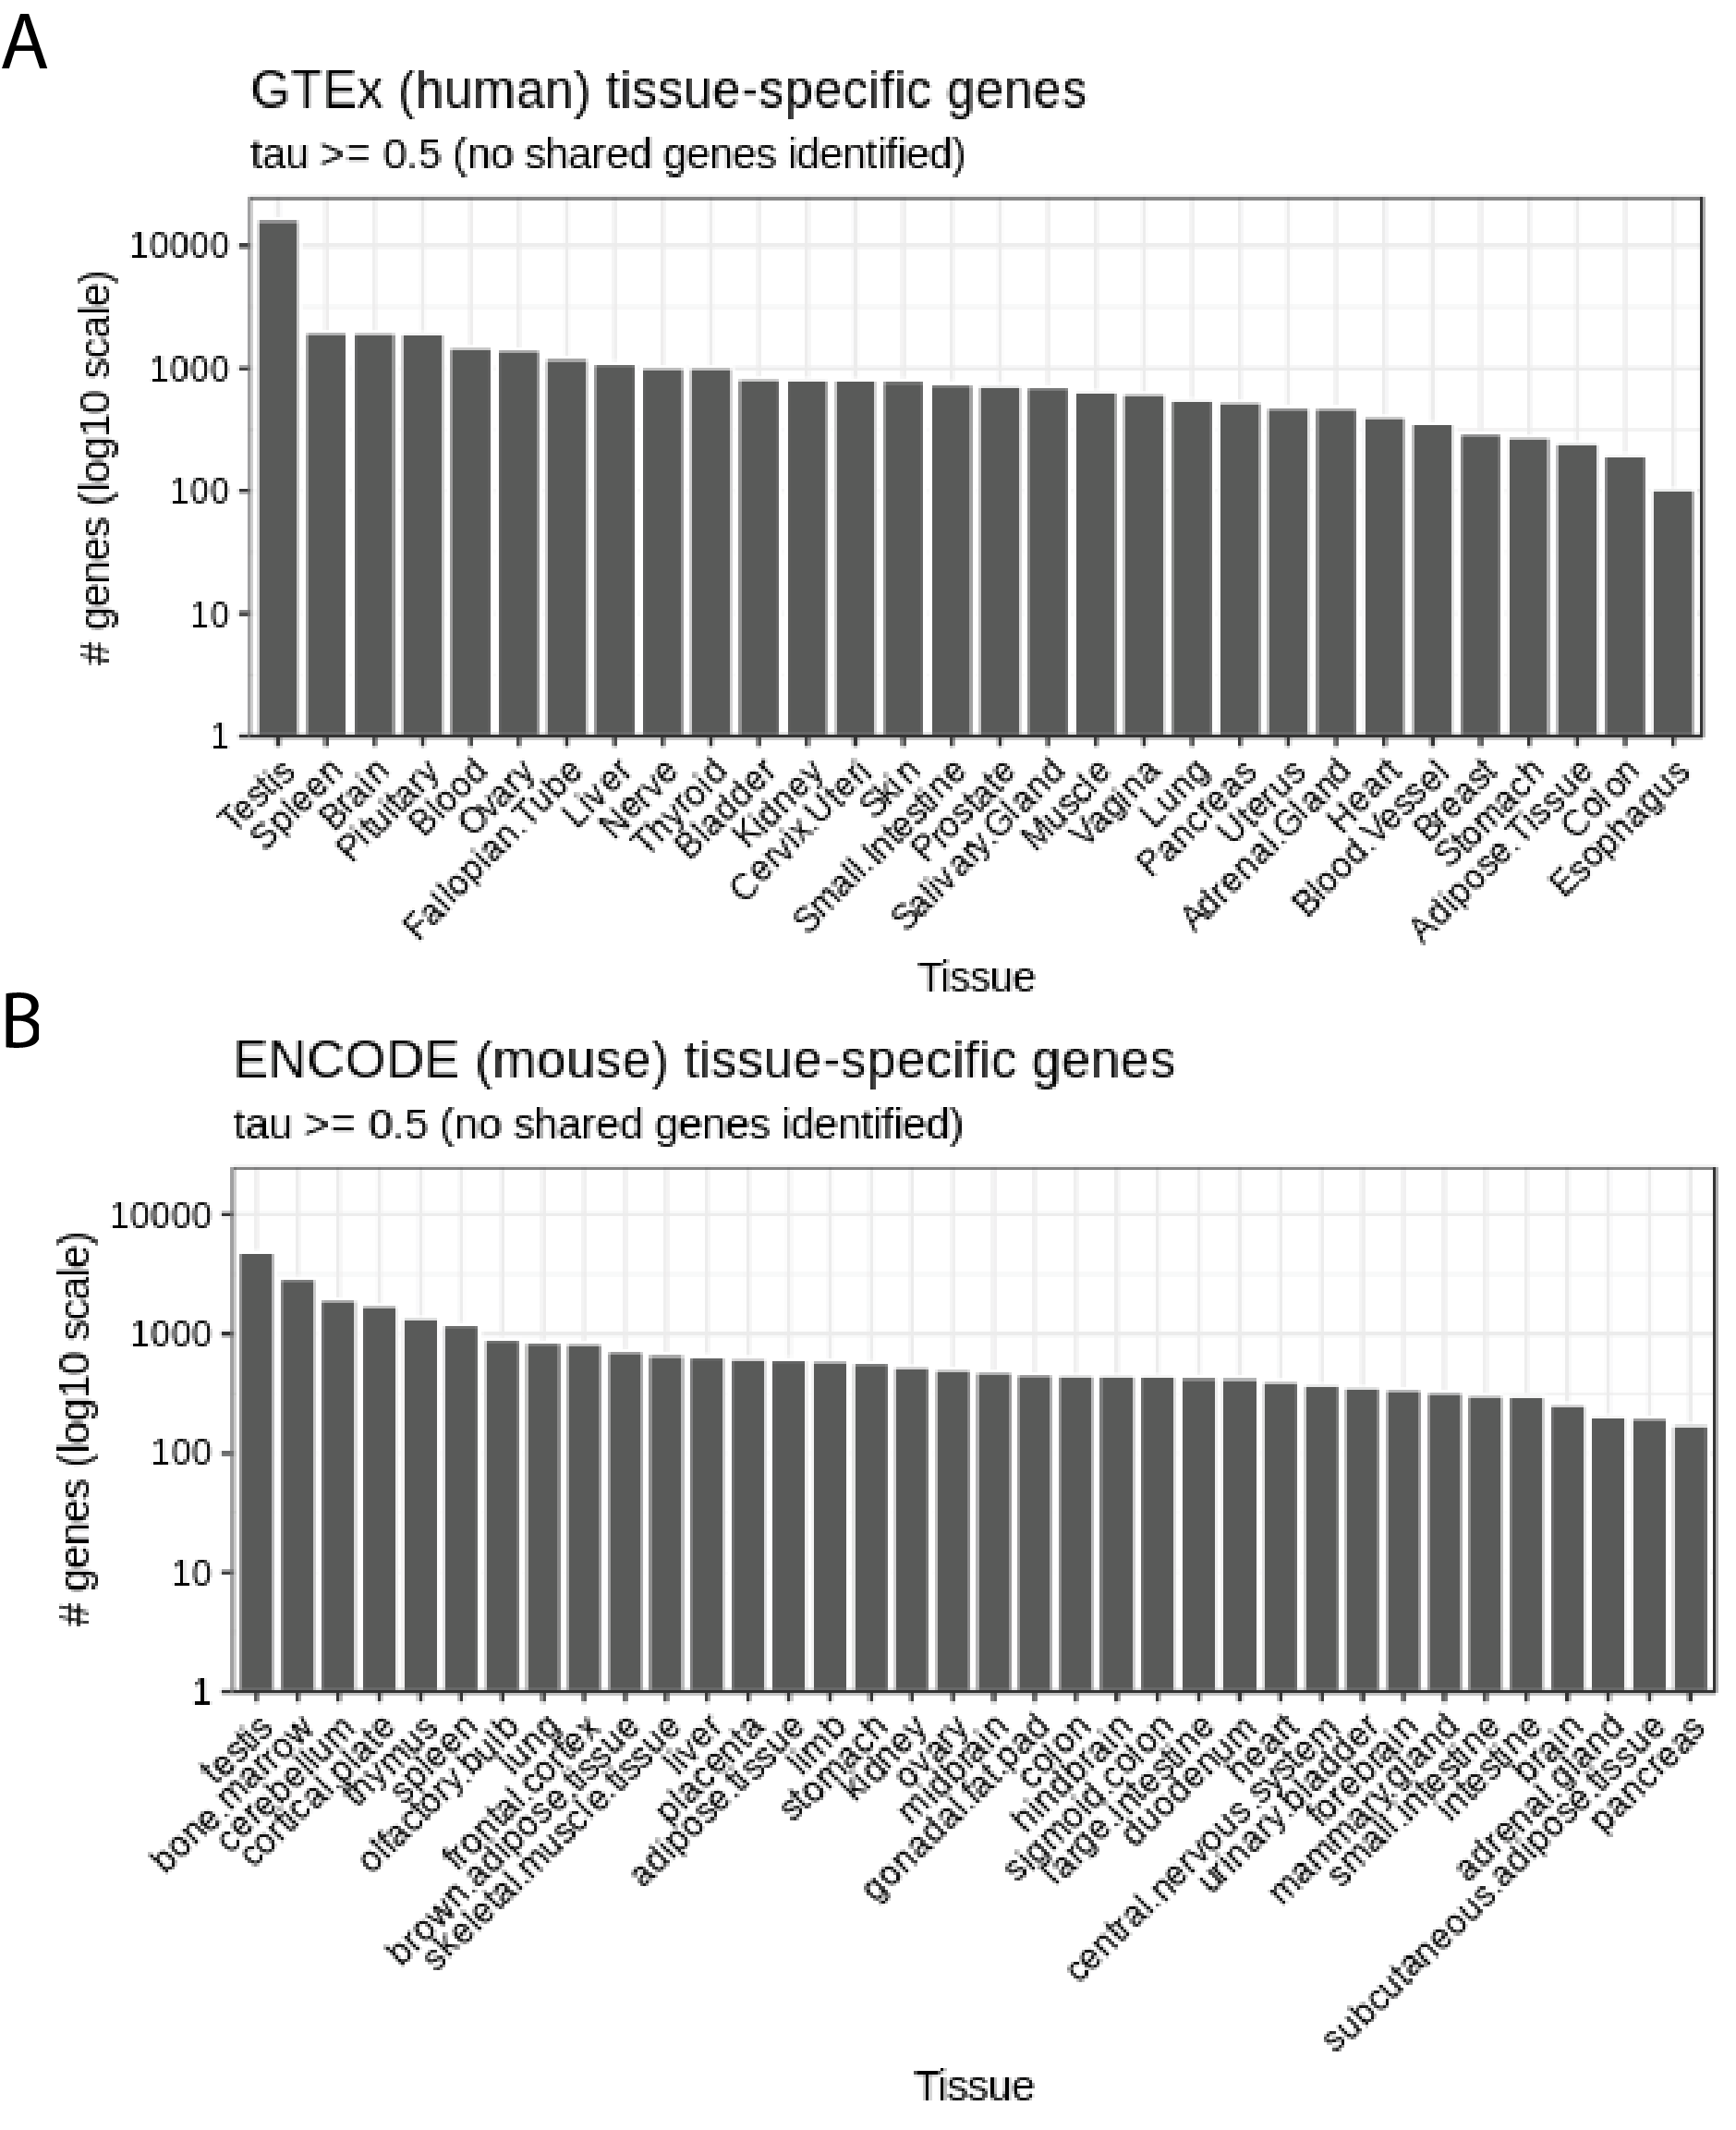
\includegraphics[width=1.0\textwidth]{Appendix3/Figs/appB_uniqueGenesTissue.png} % change word in curlies to change figure
\caption[Number of tissue-specific genes determined per tissue for mouse and human]{\textbf{Number of tissue-specific genes determined per tissue for human (A) and mouse (B))}\newline Tissue specific genes were determined by calculating tau (see Section~\ref{section4.4_genelists}) and keeping only those with a value greater than 0.5. No genes shared between tissues were found.}
\label{fig:appB_uniquegenes}
\end{figure}


\begin{figure}[hb!] 
\centering    
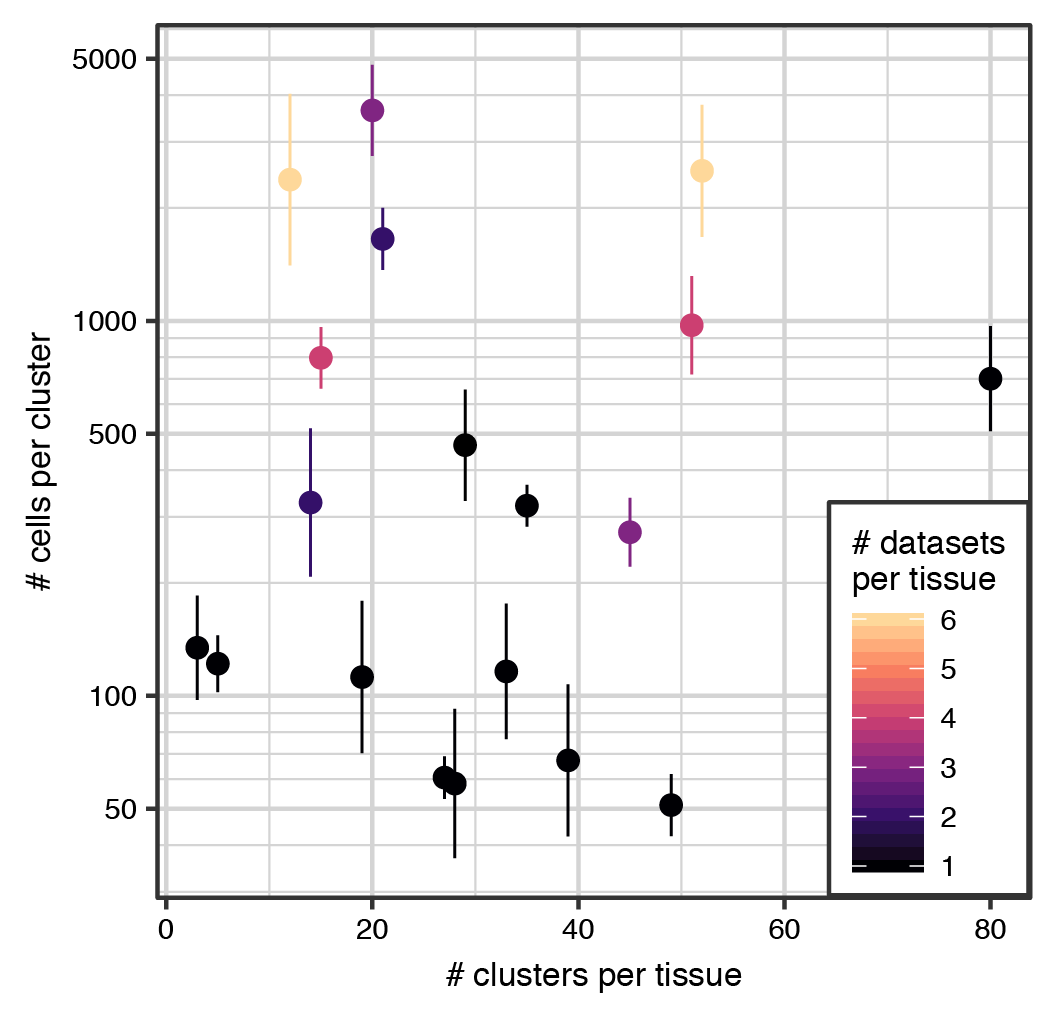
\includegraphics[scale=1.1]{Appendix3/Figs/tissue_cluster_dataset_numbers_HumanAtlas.png} % change word in curlies to change figure
\caption[Relating number of per-tissue clusters and number of cells]{\textbf{Relating number of per-tissue clusters and number of cells (Related to Figure~\ref{fig:chap3_HA}A)}\newline Scatter plot showing the variation of number of clusters per tissue with the number of cells, as well as number of datasets collected for each tissue (colour).}
\label{fig:appB_clustnumbs}
\end{figure}


\begin{figure}[ht!] 
\centering
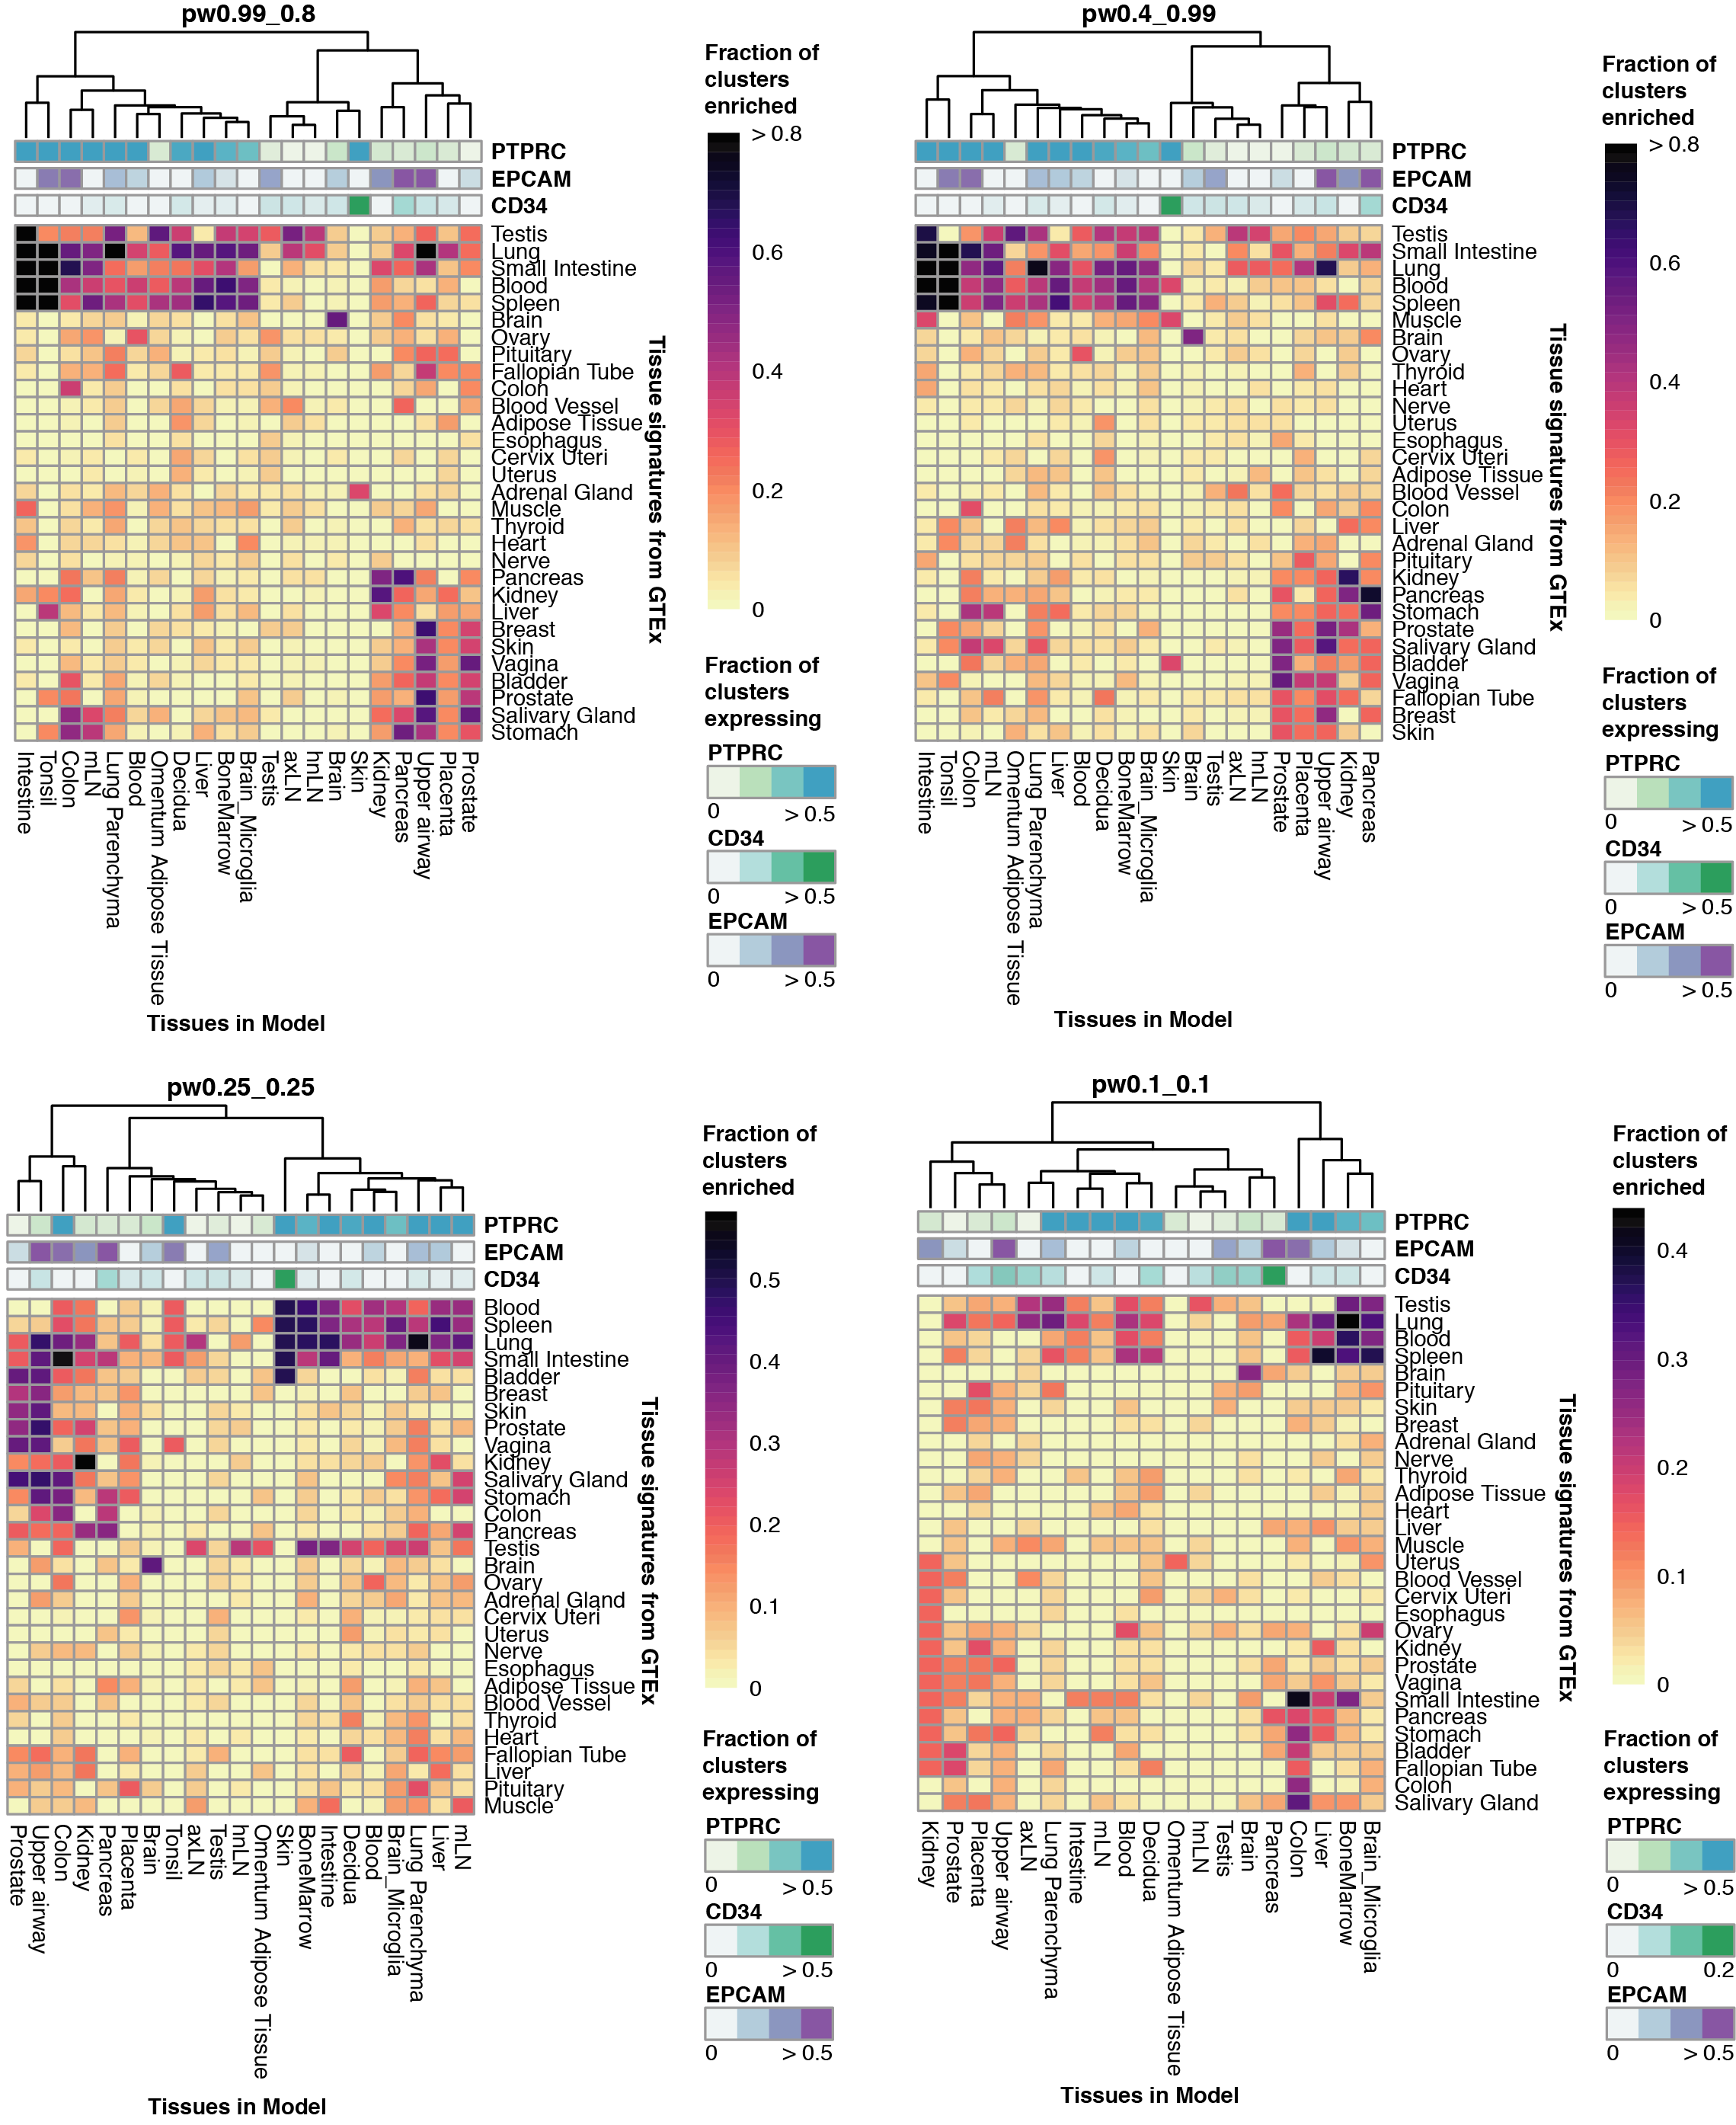
\includegraphics[scale=0.77]{Appendix3/Figs/appB_tissueGSEA.png} % change word in curlies to change figure
\caption[Enrichment of tissue gene modules in other \textit{CellTypist} models]{\textbf{Enrichment of tissue gene modules in other \textit{CellTypist} models (Related to Figure~\ref{fig:chap4_tiss})}\newline Heatmaps showing the fraction of clusters in each tissue (x-axis) with an enrichment for tissue-specific gene programmes (y-axis) determined from GTEx data. Each heatmap represents a different set of clusters per tissue, resulting from using different parameters in the \textit{CellTypist} pipeline. Plot for thr1 = 0.99, thr2 = 0.8 is identical to Figure~\ref{fig:chap4_tiss}B.}
\label{fig:appB_tissGSEA}
\end{figure}


\begin{figure}[ht!] 
\centering
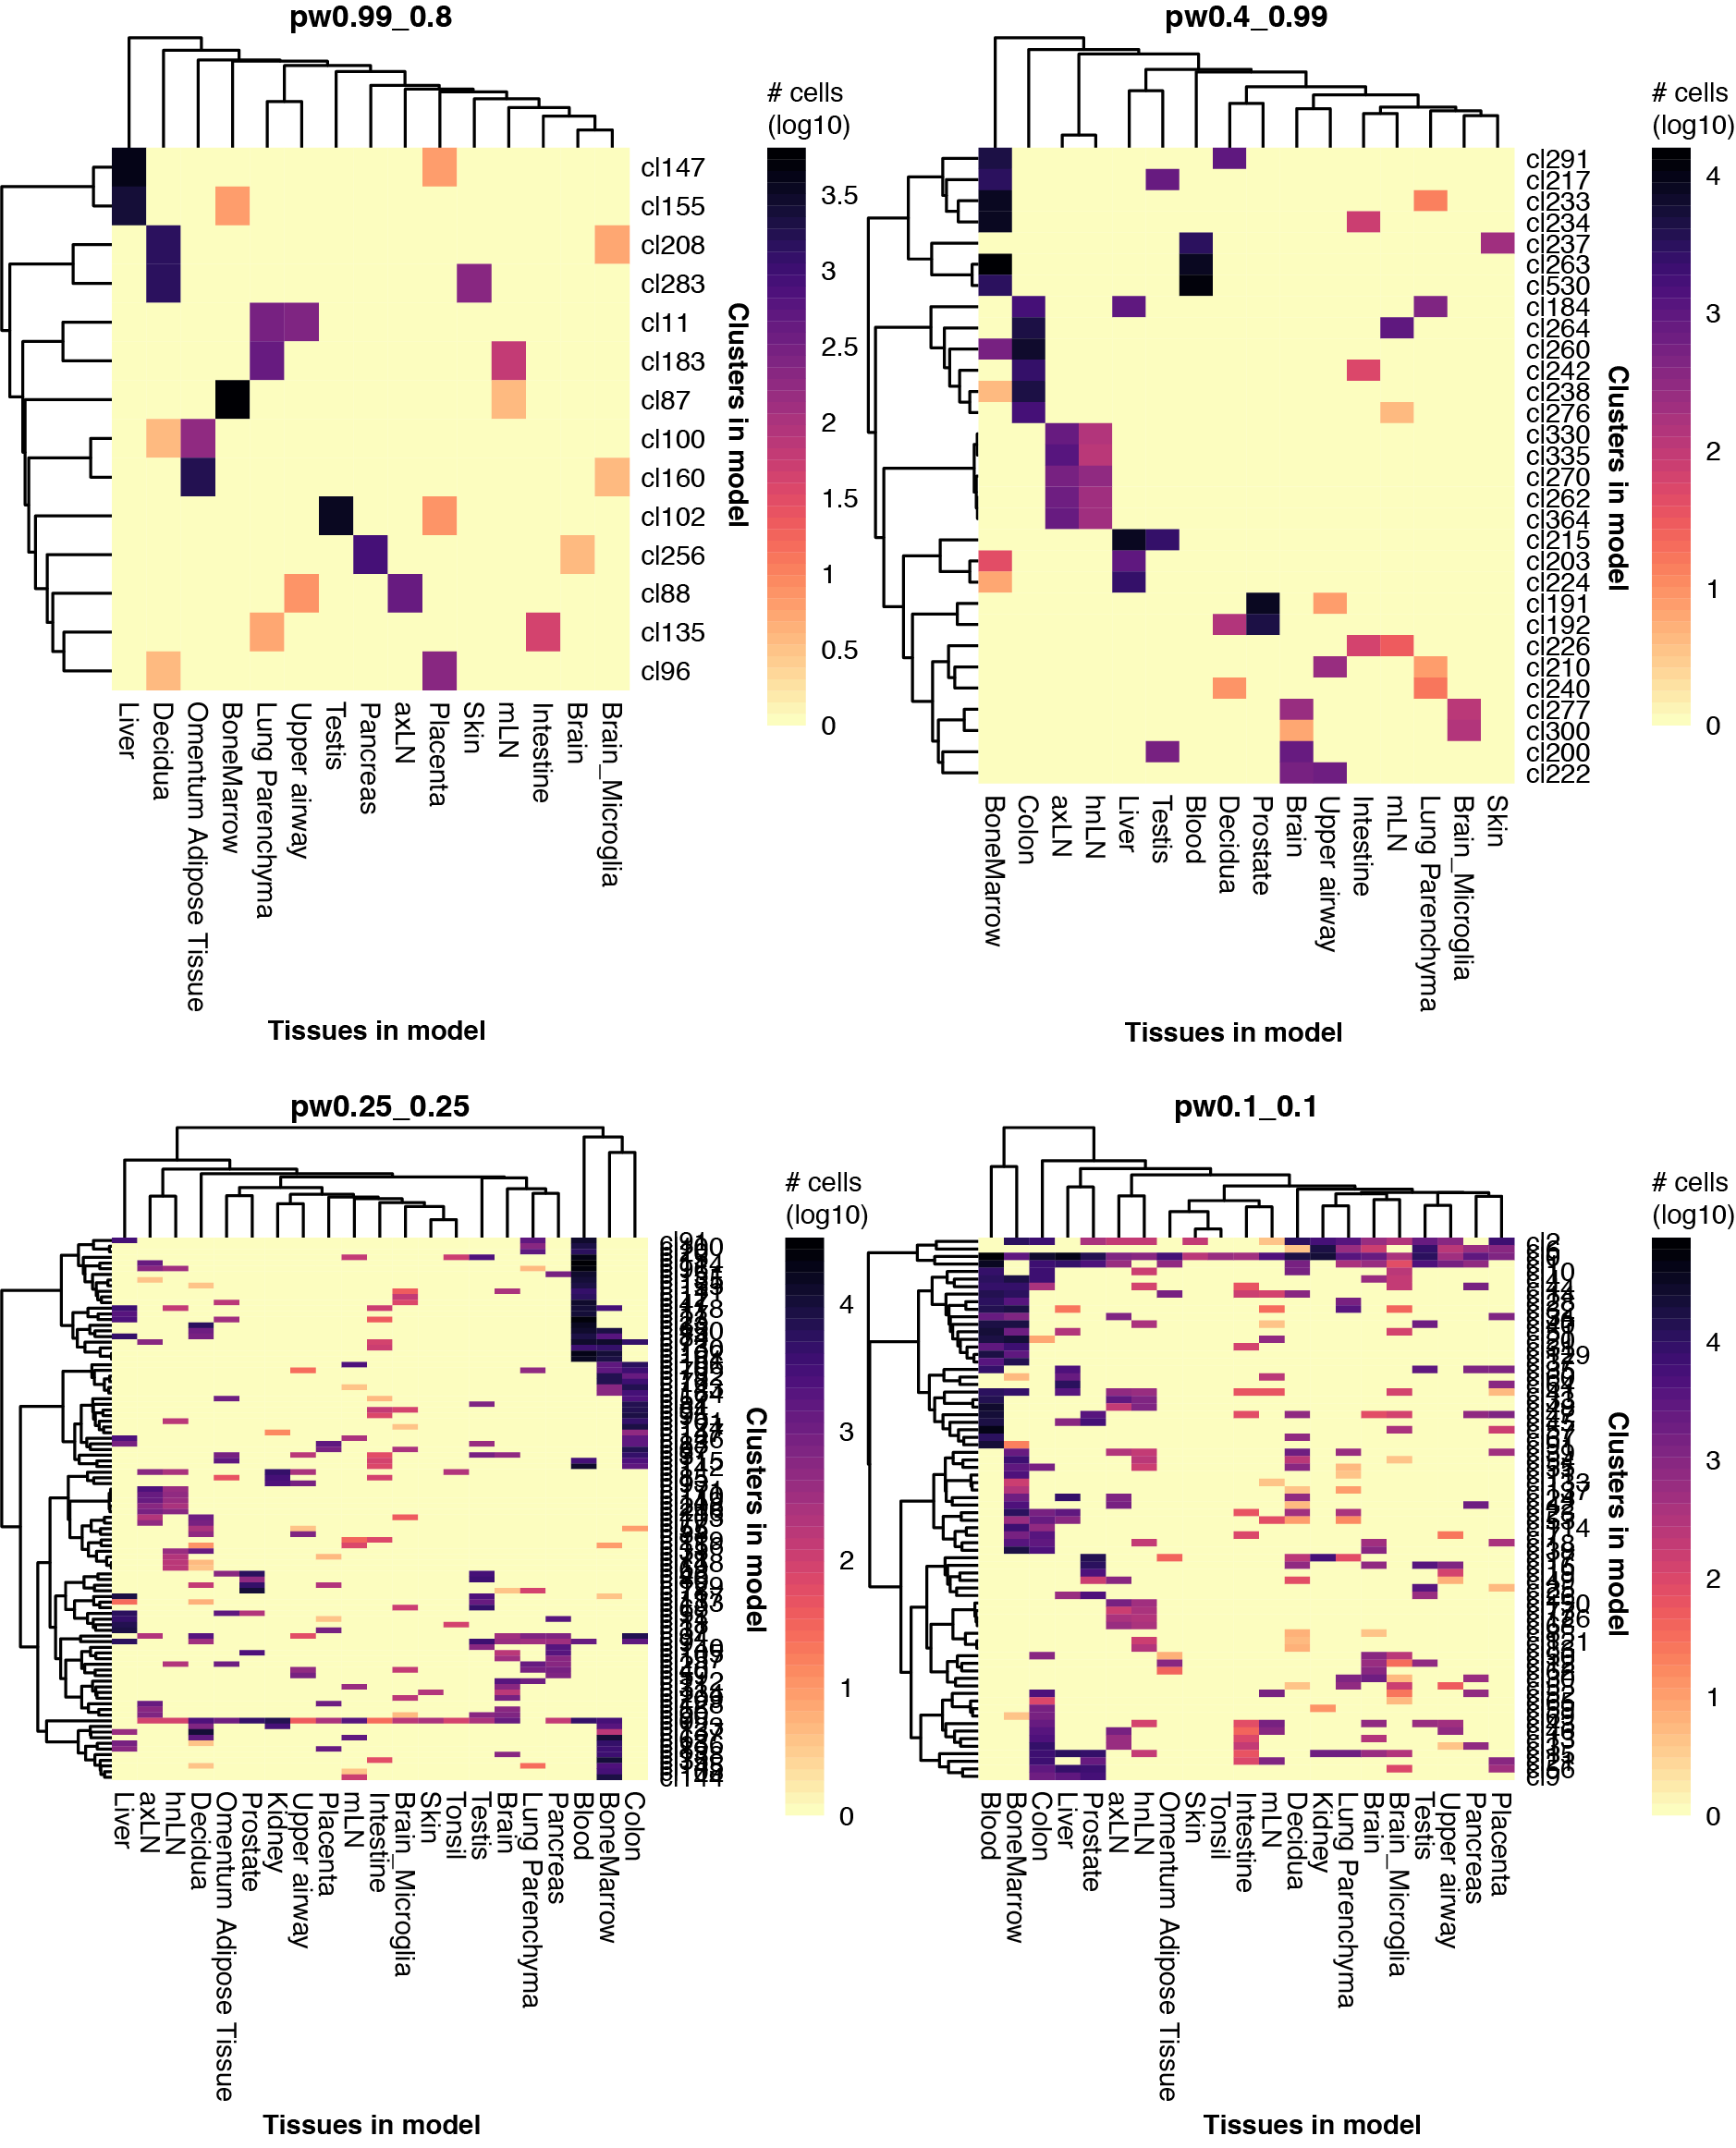
\includegraphics[width=1.0\textwidth]{Appendix3/Figs/appB_tissue_clustrelations_HumanAtlas.png} % change word in curlies to change figure
\caption[Clusters merged across tissues in the different models]{\textbf{Clusters merged across tissues in the different models (Related to Figure~\ref{fig:chap4_tiss})}\newline Heatmaps showing the number of cells contributed by each tissue into cross-tissue clusters for each model.}
\label{fig:appC_tissrel}
\end{figure}


\begin{figure}[ht!] 
\centering
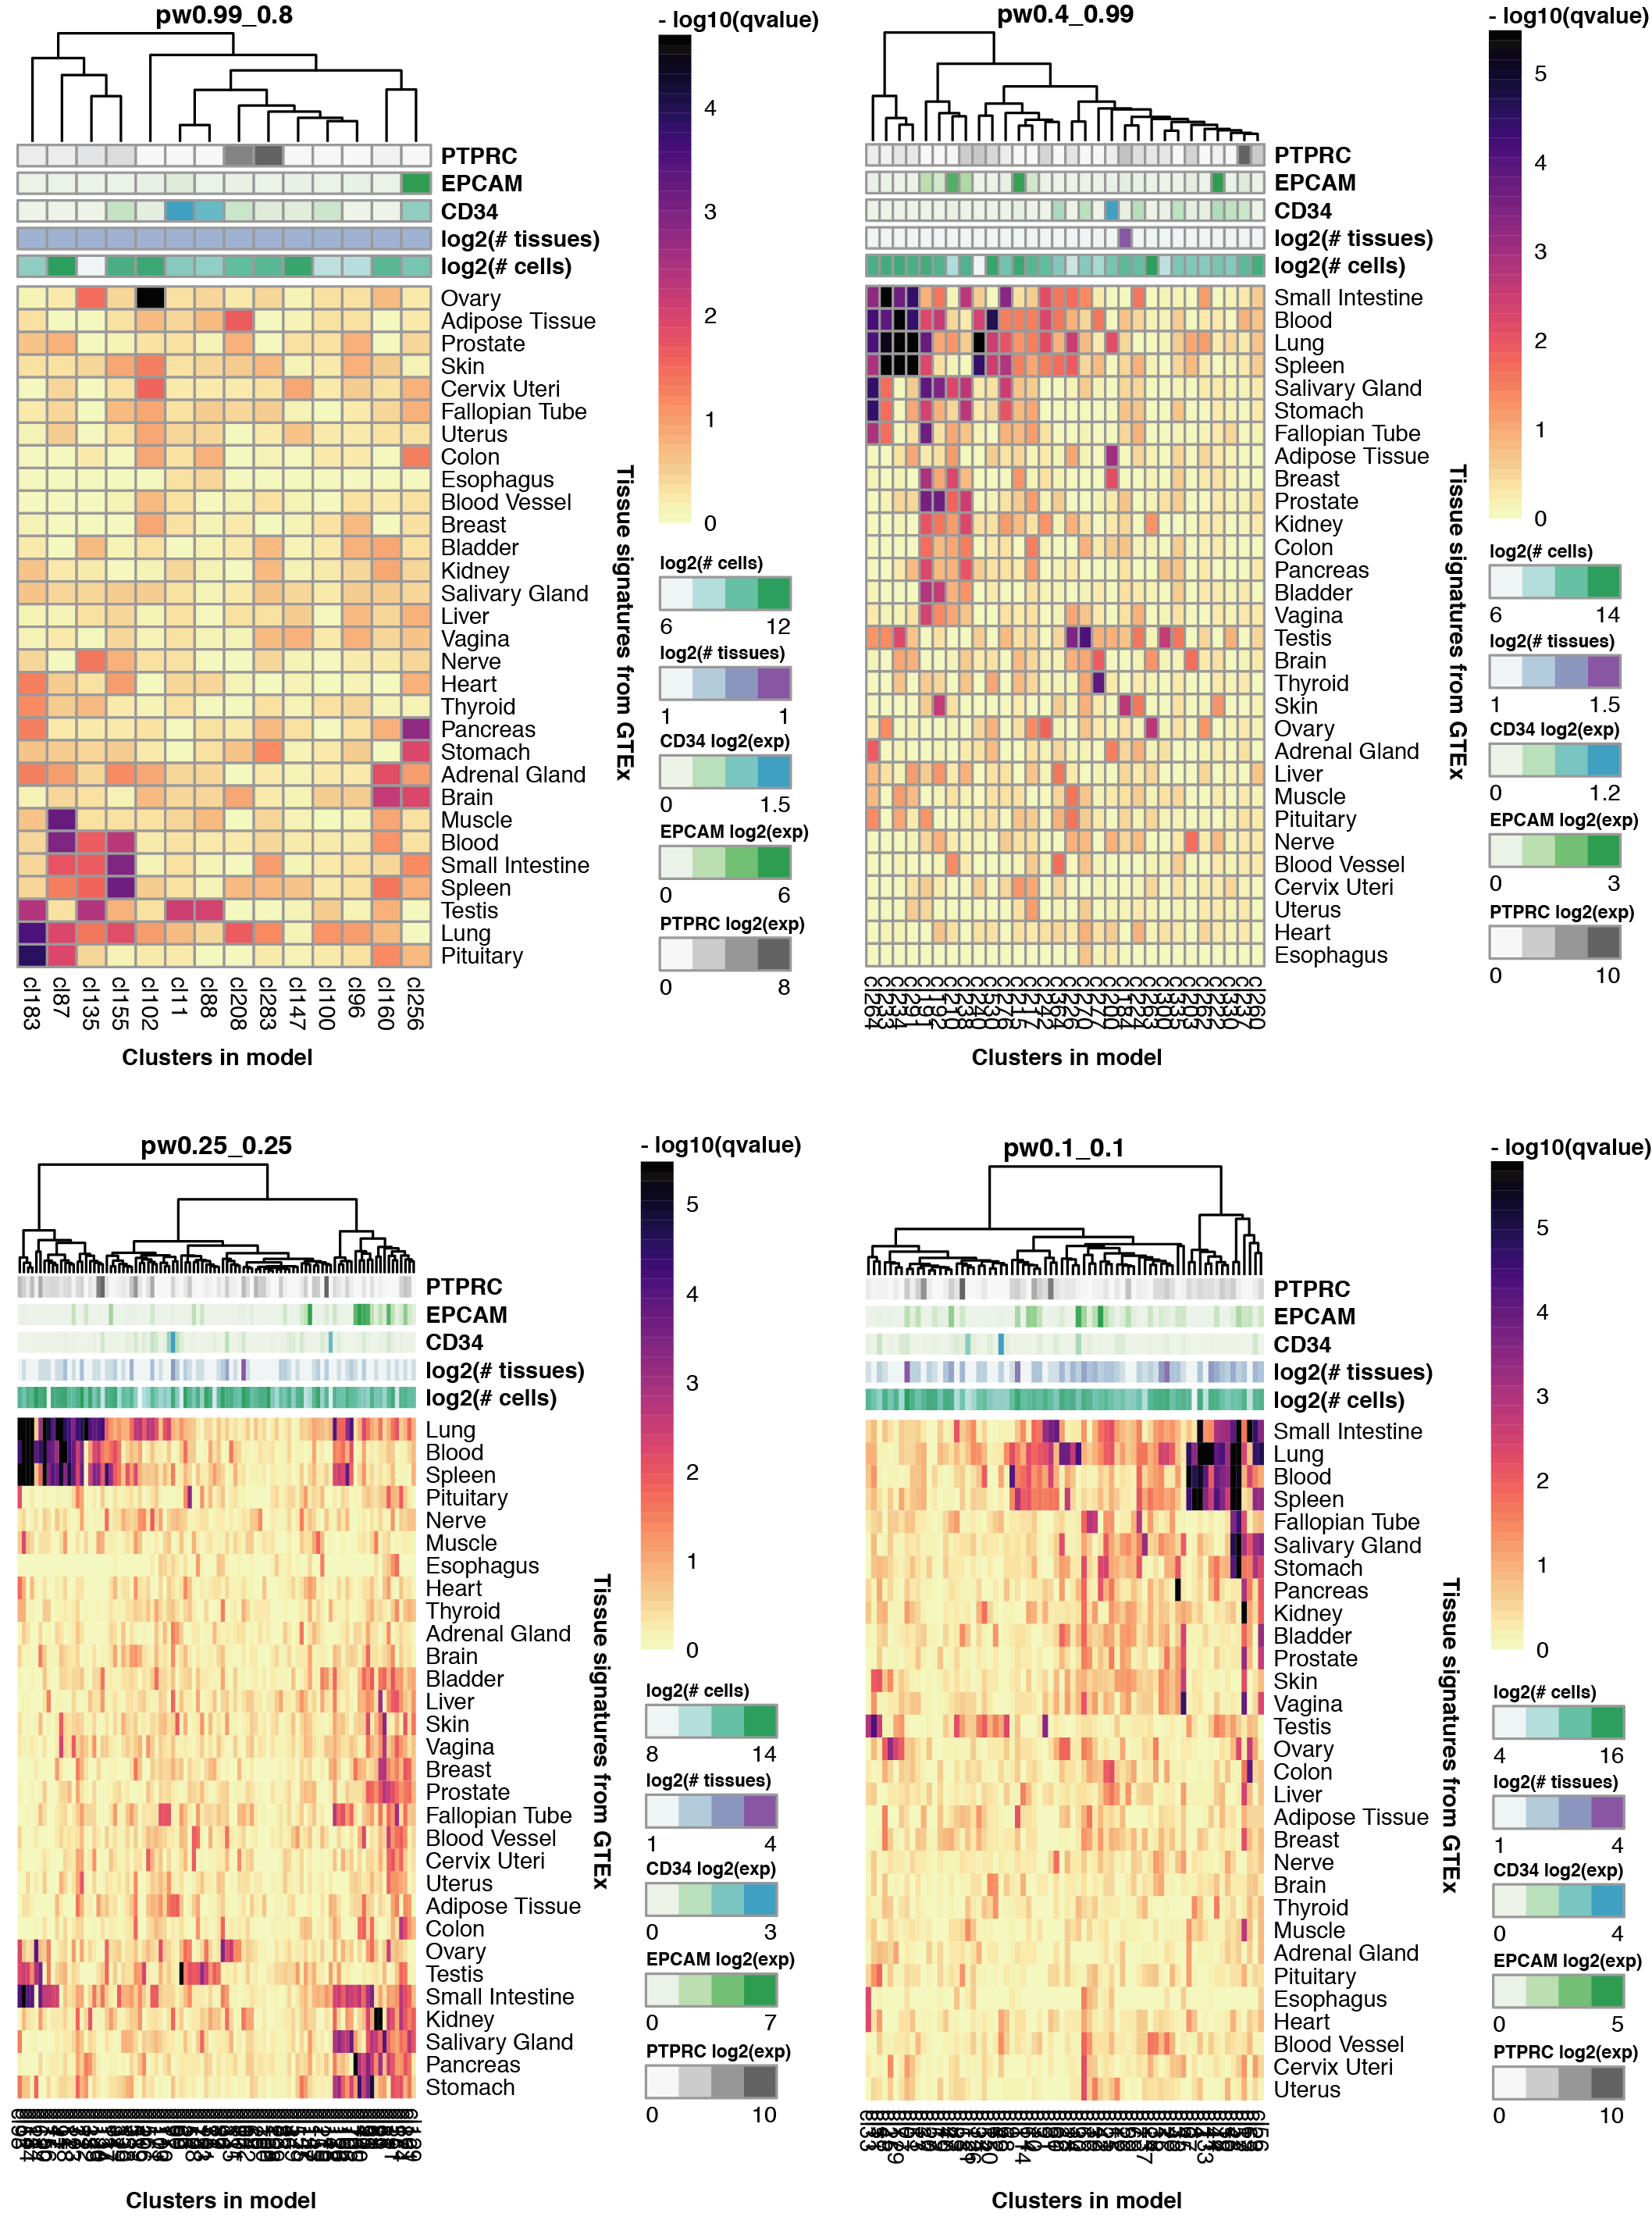
\includegraphics[scale=0.77]{Appendix3/Figs/appB_clmGSEA.png} % change word in curlies to change figure
\caption[Enrichment of tissue gene modules in merged clusters of different \textit{CellTypist} models]{\textbf{Enrichment of tissue gene modules in merged clusters of different \textit{CellTypist} models (Related to Figure~\ref{fig:chap4_tiss})}\newline Heatmaps showing the -log10(q-value) of each merged cluster (x-axis) for the enrichment of tissue-specific gene programmes (y-axis) in their top 500 genes output by the model. Each heatmap represents a different set of merged clusters, resulting from using different parameters in the \textit{CellTypist} pipeline.}
\label{fig:appB_clmGSEA}
\end{figure}


\begin{figure}[ht!] 
\centering
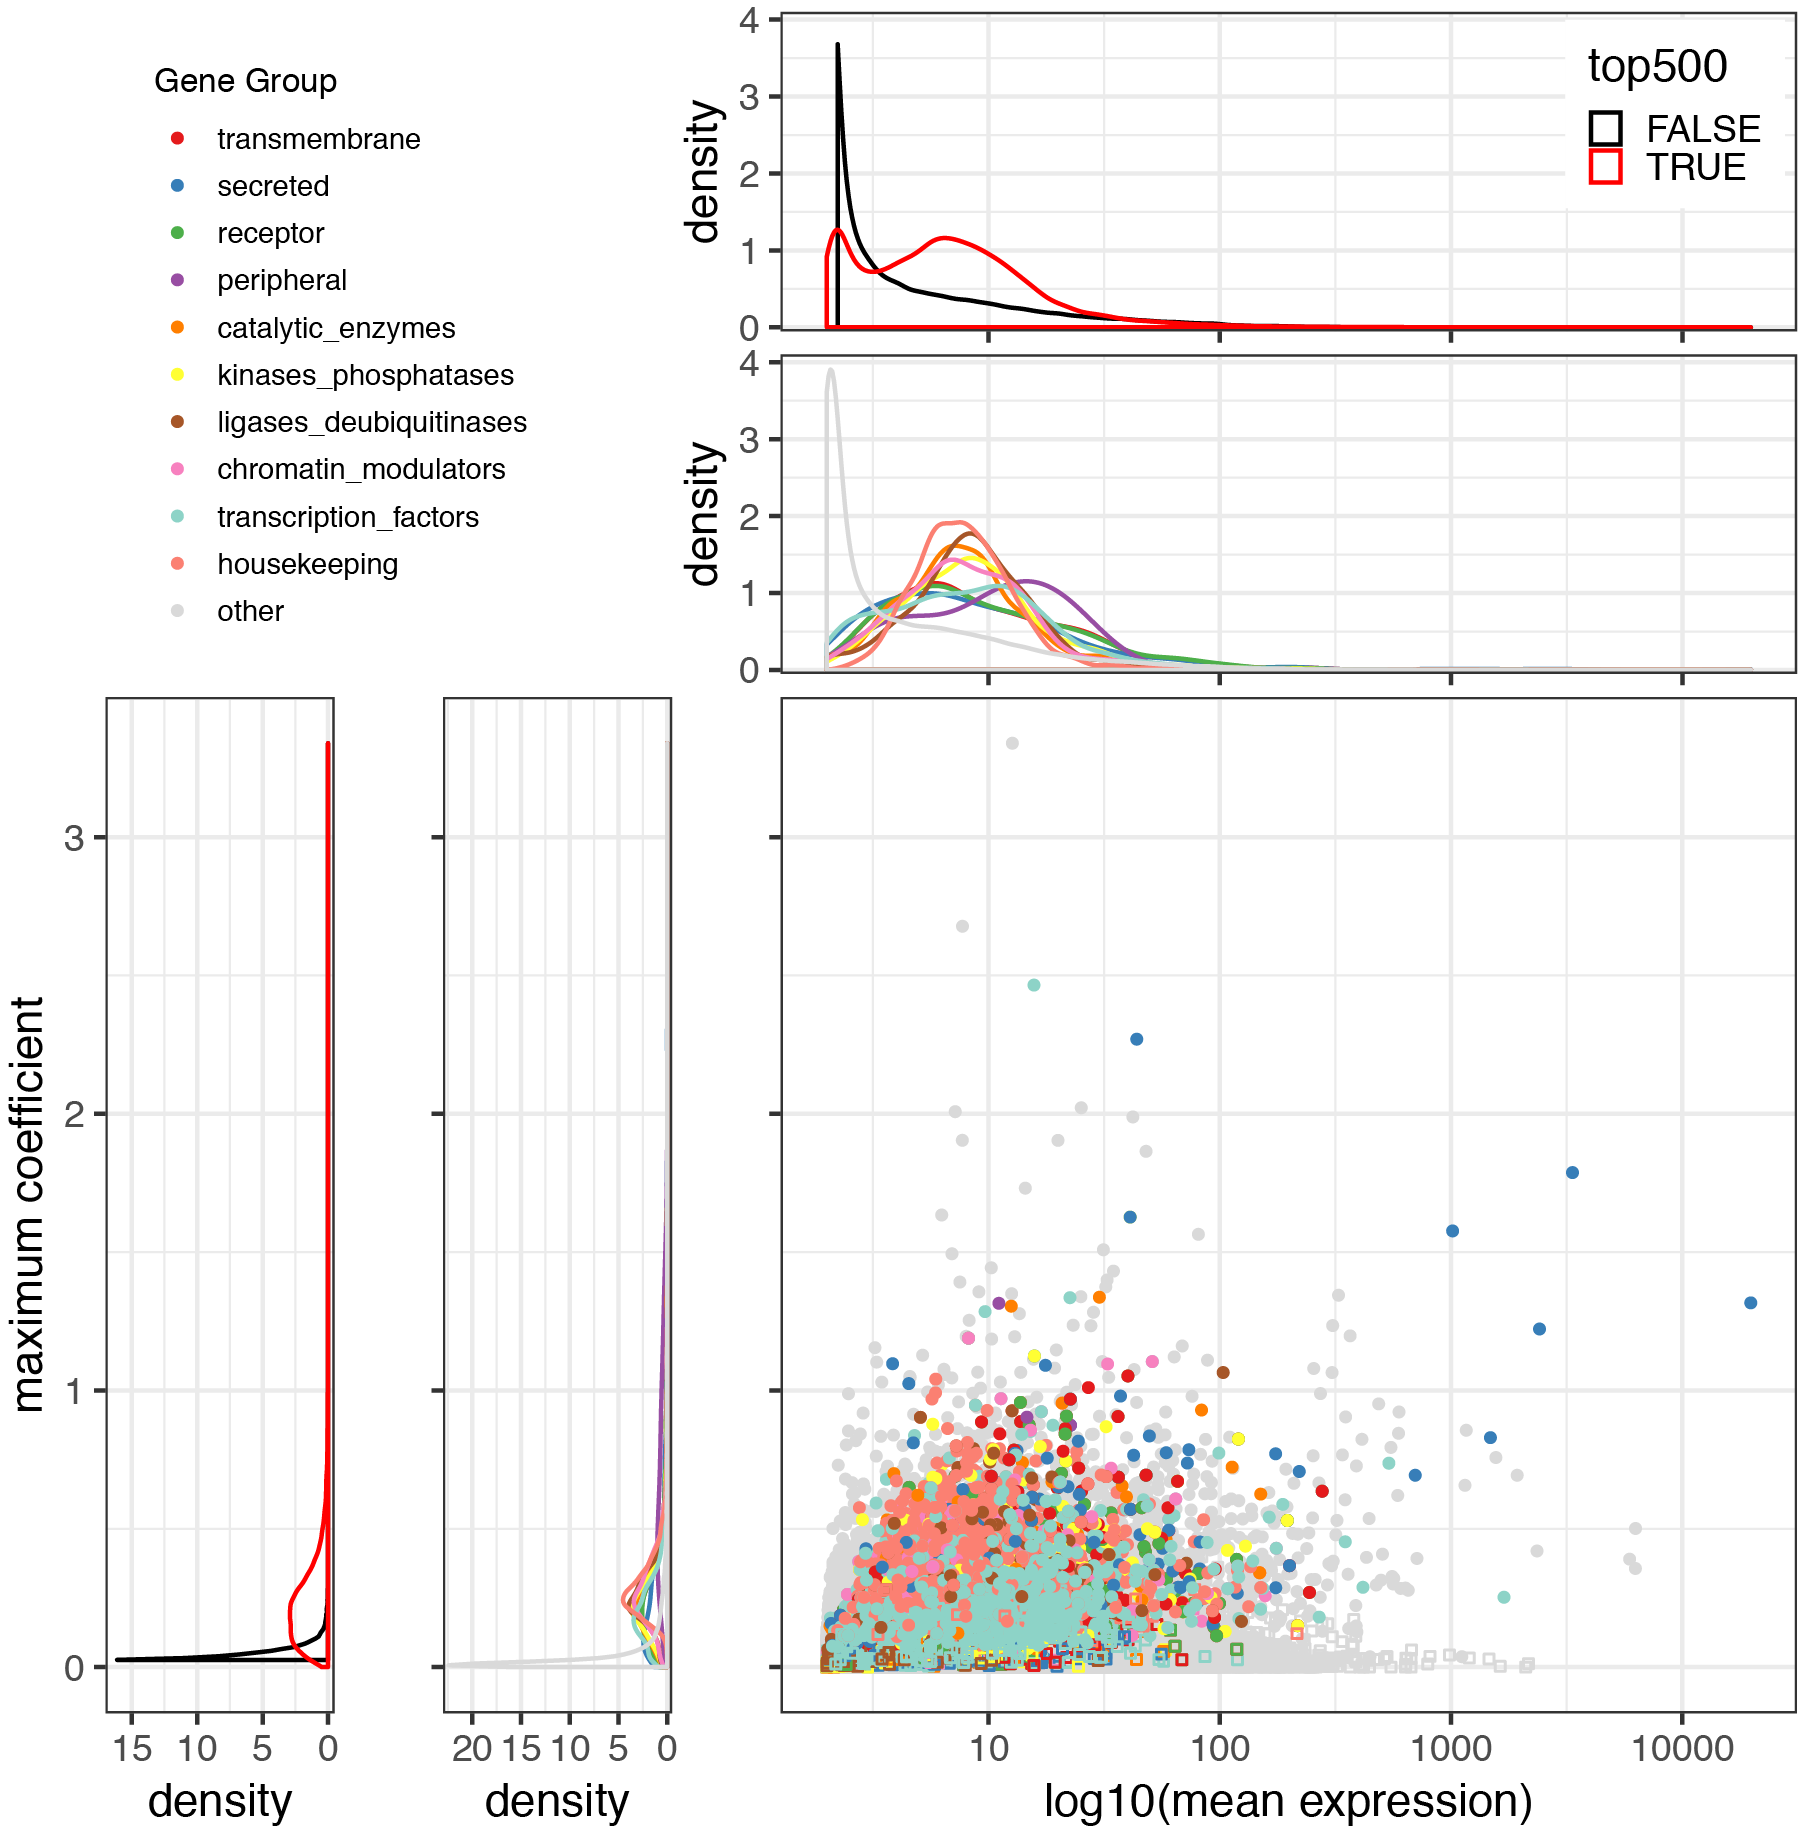
\includegraphics[scale=0.9]{Appendix3/Figs/gene_coeff_exp_HumanAtlas.png} % change word in curlies to change figure
\caption[Correlation between gene expression and importance in the human \textit{CellTypist} model]{\textbf{Correlation between gene expression and importance in the human \textit{CellTypist} model (Related to Figure~\ref{fig:chap4_genetypes})}\newline Scatterplot shows the relationship between mean expression across all cells and the maximum coefficient for each gene across all labels. Density plots show distribution of gene groups, and distribution of genes included in the top 500 coefficients of any label, along the mean expression (top) or maximum coefficient (left) range. Spearman correlation coefficient = 0.56, p-value < 0.01.}
\label{fig:appB_human_coeff_exp}
\end{figure}


\begin{figure}[ht!] 
\centering
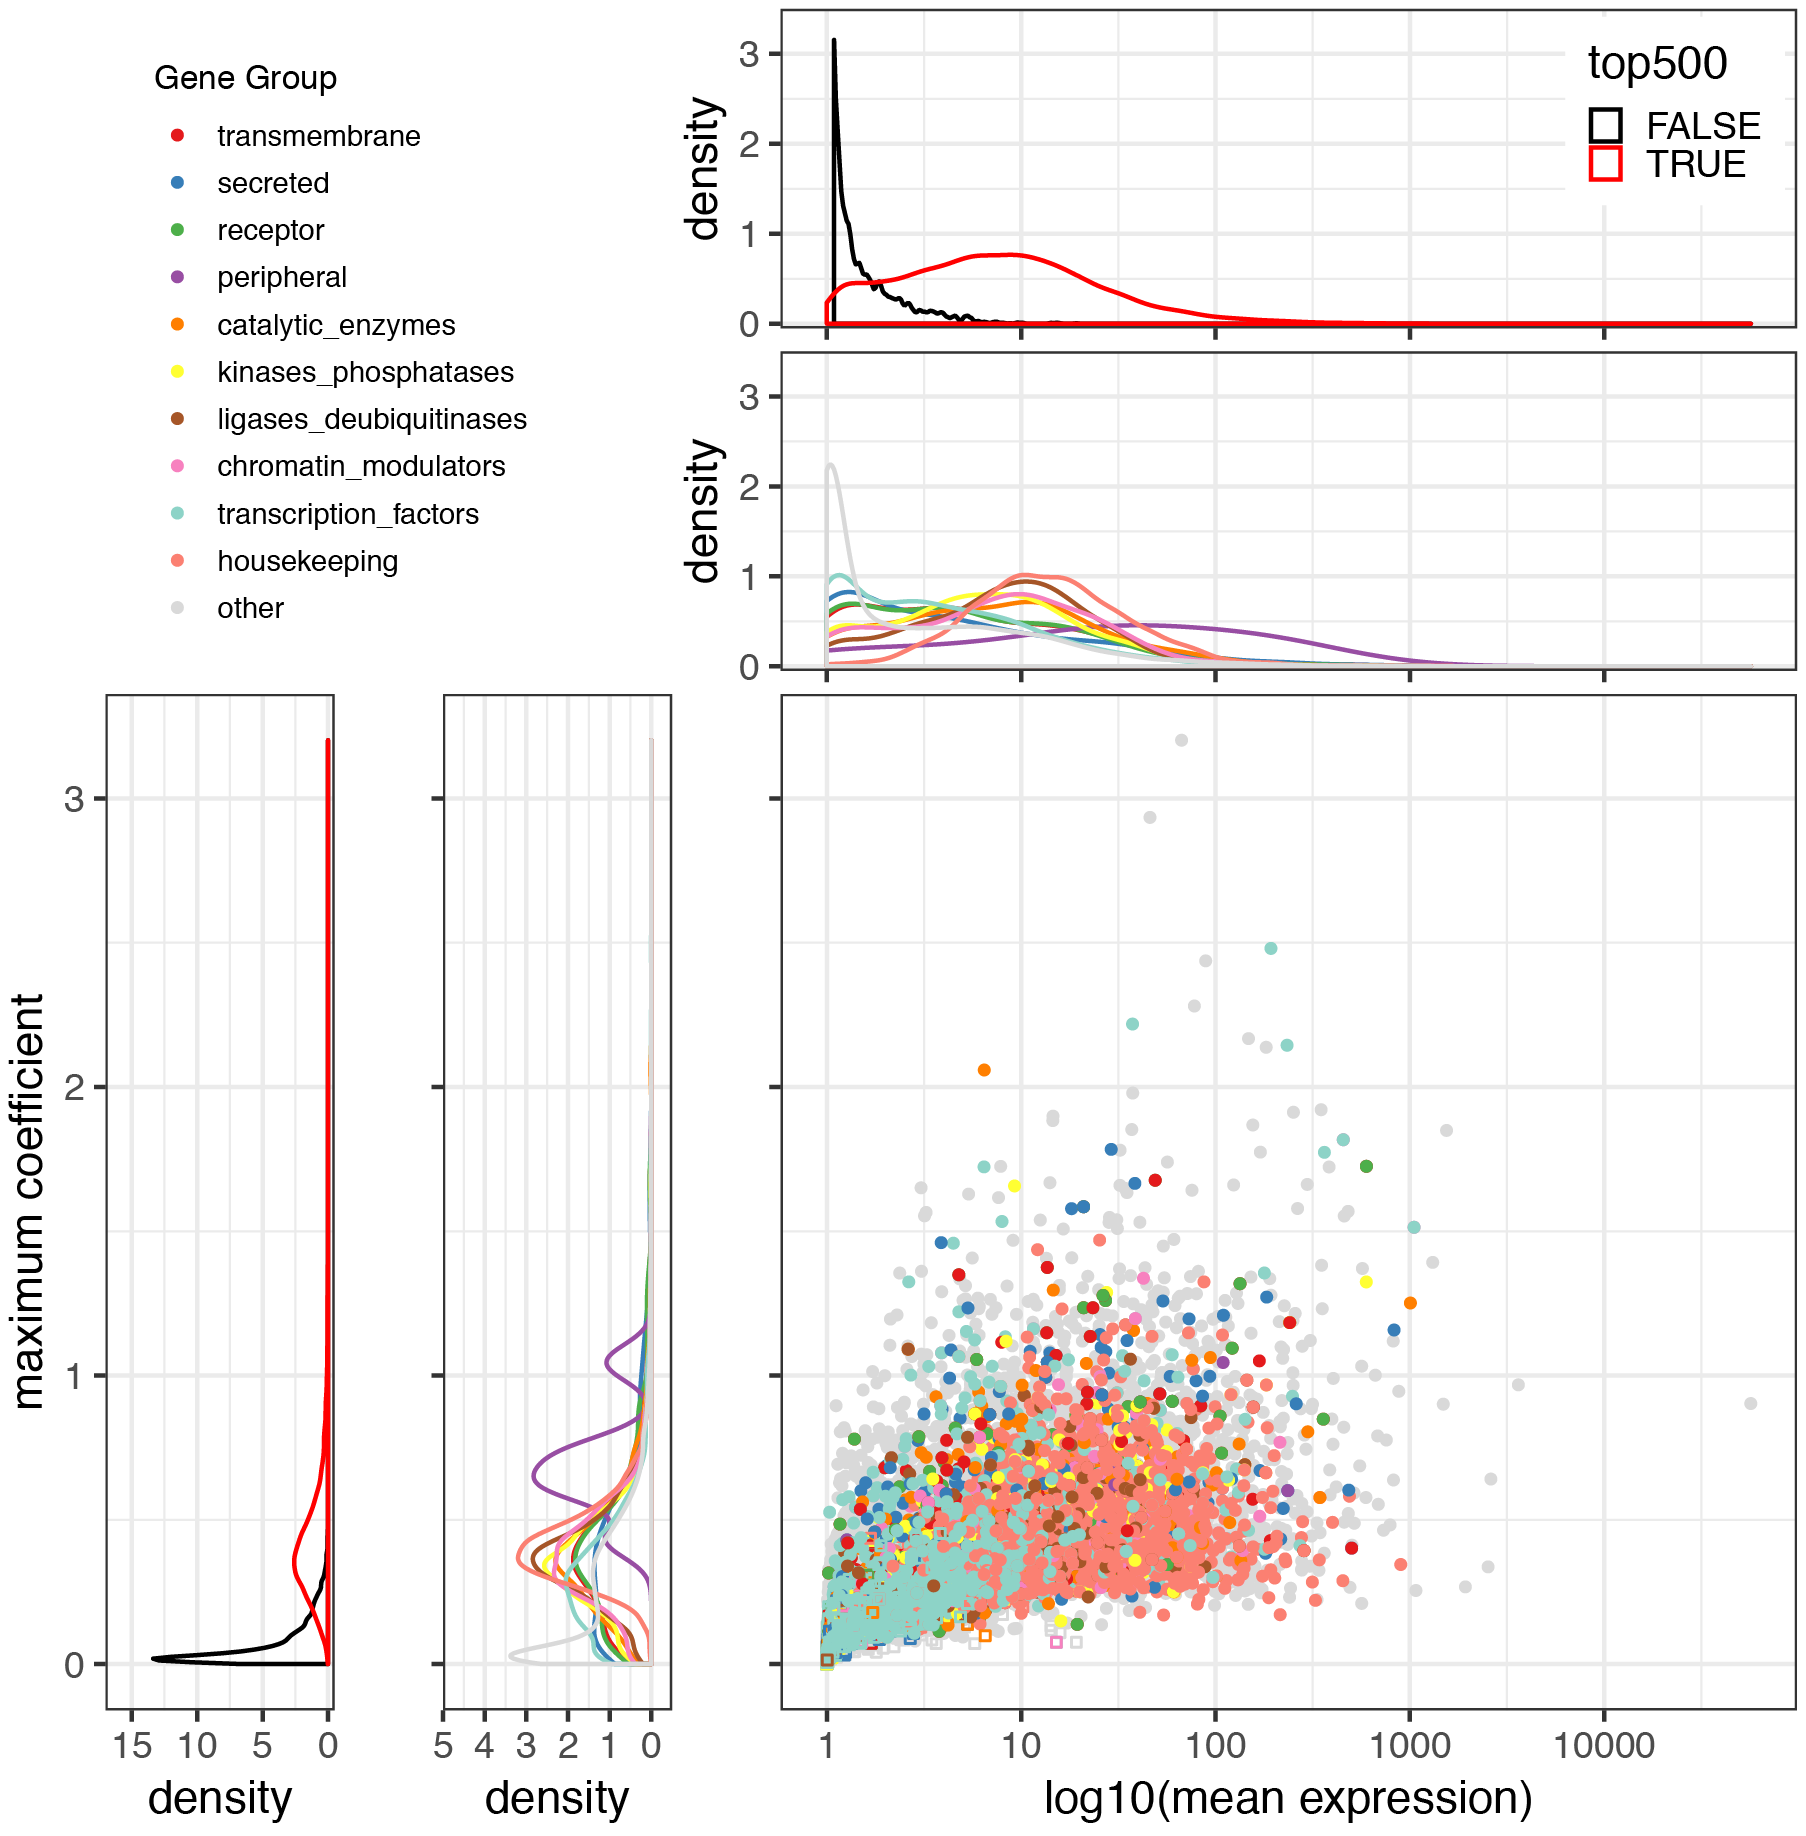
\includegraphics[scale=0.9]{Appendix3/Figs/gene_coeff_exp_TabulaMuris.png} % change word in curlies to change figure
\caption[Correlation between gene expression and importance in the \textit{Tabula Muris} \textit{CellTypist} model]{\textbf{Correlation between gene expression and importance in the \textit{Tabula Muris} \textit{CellTypist} model (Related to Figure~\ref{fig:chap4_genetypes_mouse})}\newline Scatterplot shows the relationship between mean expression across all cells and the maximum coefficient for each gene across all labels. Density plots show distribution of gene groups, and distribution of genes included in the top 500 coefficients of any label, along the mean expression (top) or maximum coefficient (left) range. Spearman correlation coefficient = 0.86, p-value < 0.01.}
\label{fig:appB_mouse_coeff_exp}
\end{figure}


\begin{figure}[ht!] 
\centering
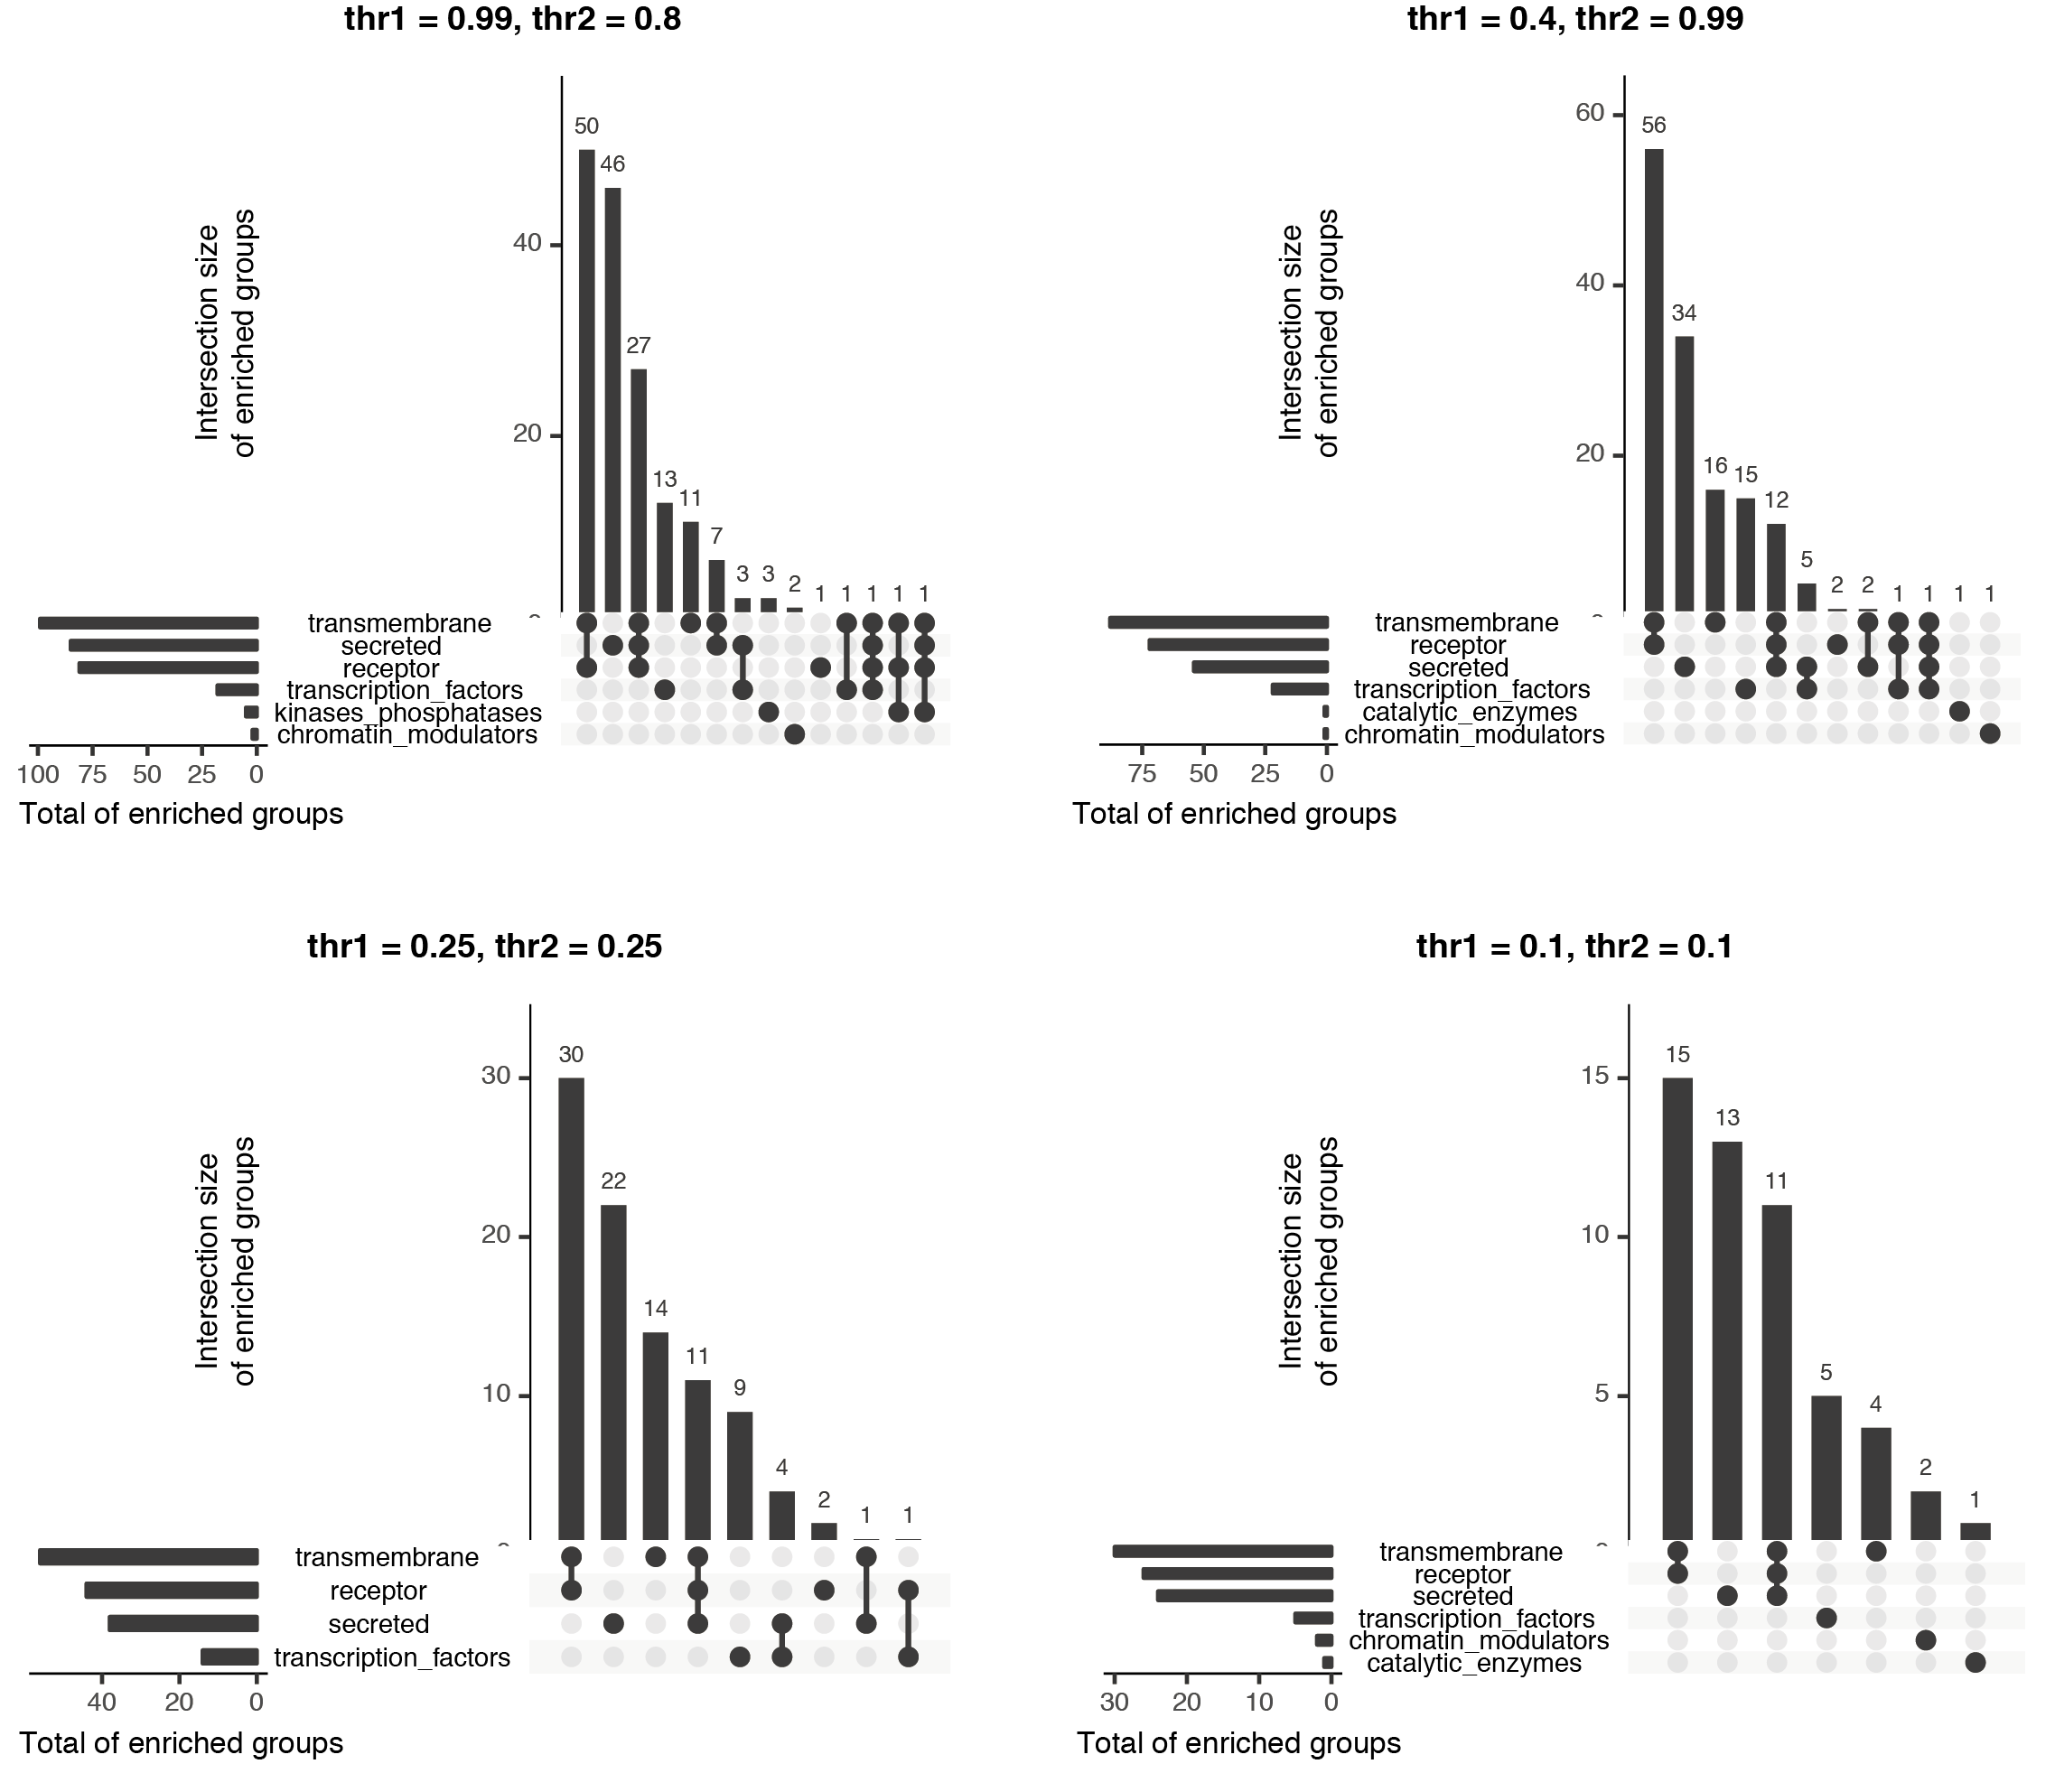
\includegraphics[scale=0.79]{Appendix3/Figs/appB_upset.png} % change word in curlies to change figure
\caption[Gene upset plots of different \textit{CellTypist} models]{\textbf{Gene upset plots of different \textit{CellTypist} models (Related to Figure~\ref{fig:chap4_genetypes})}\newline Upset plots counting the number of clusters enriched for a specific group of genes in each model. The gene groups tested were "transcription factors", "transmembrane", "secreted", "receptors", "membrane peripheral proteins", "kinases and phosphatases", "chromatin modulators", "catalytic enzymes", "housekeeping genes". Only the terms enriched in at least one cluster were shown. The plot for thr1 = 0.99, thr2 = 0.8 is identical to Figure~\ref{fig:chap4_genetypes}B.}
\label{fig:appB_supupset}
\end{figure}


\begin{figure}[pht!] 
\centering
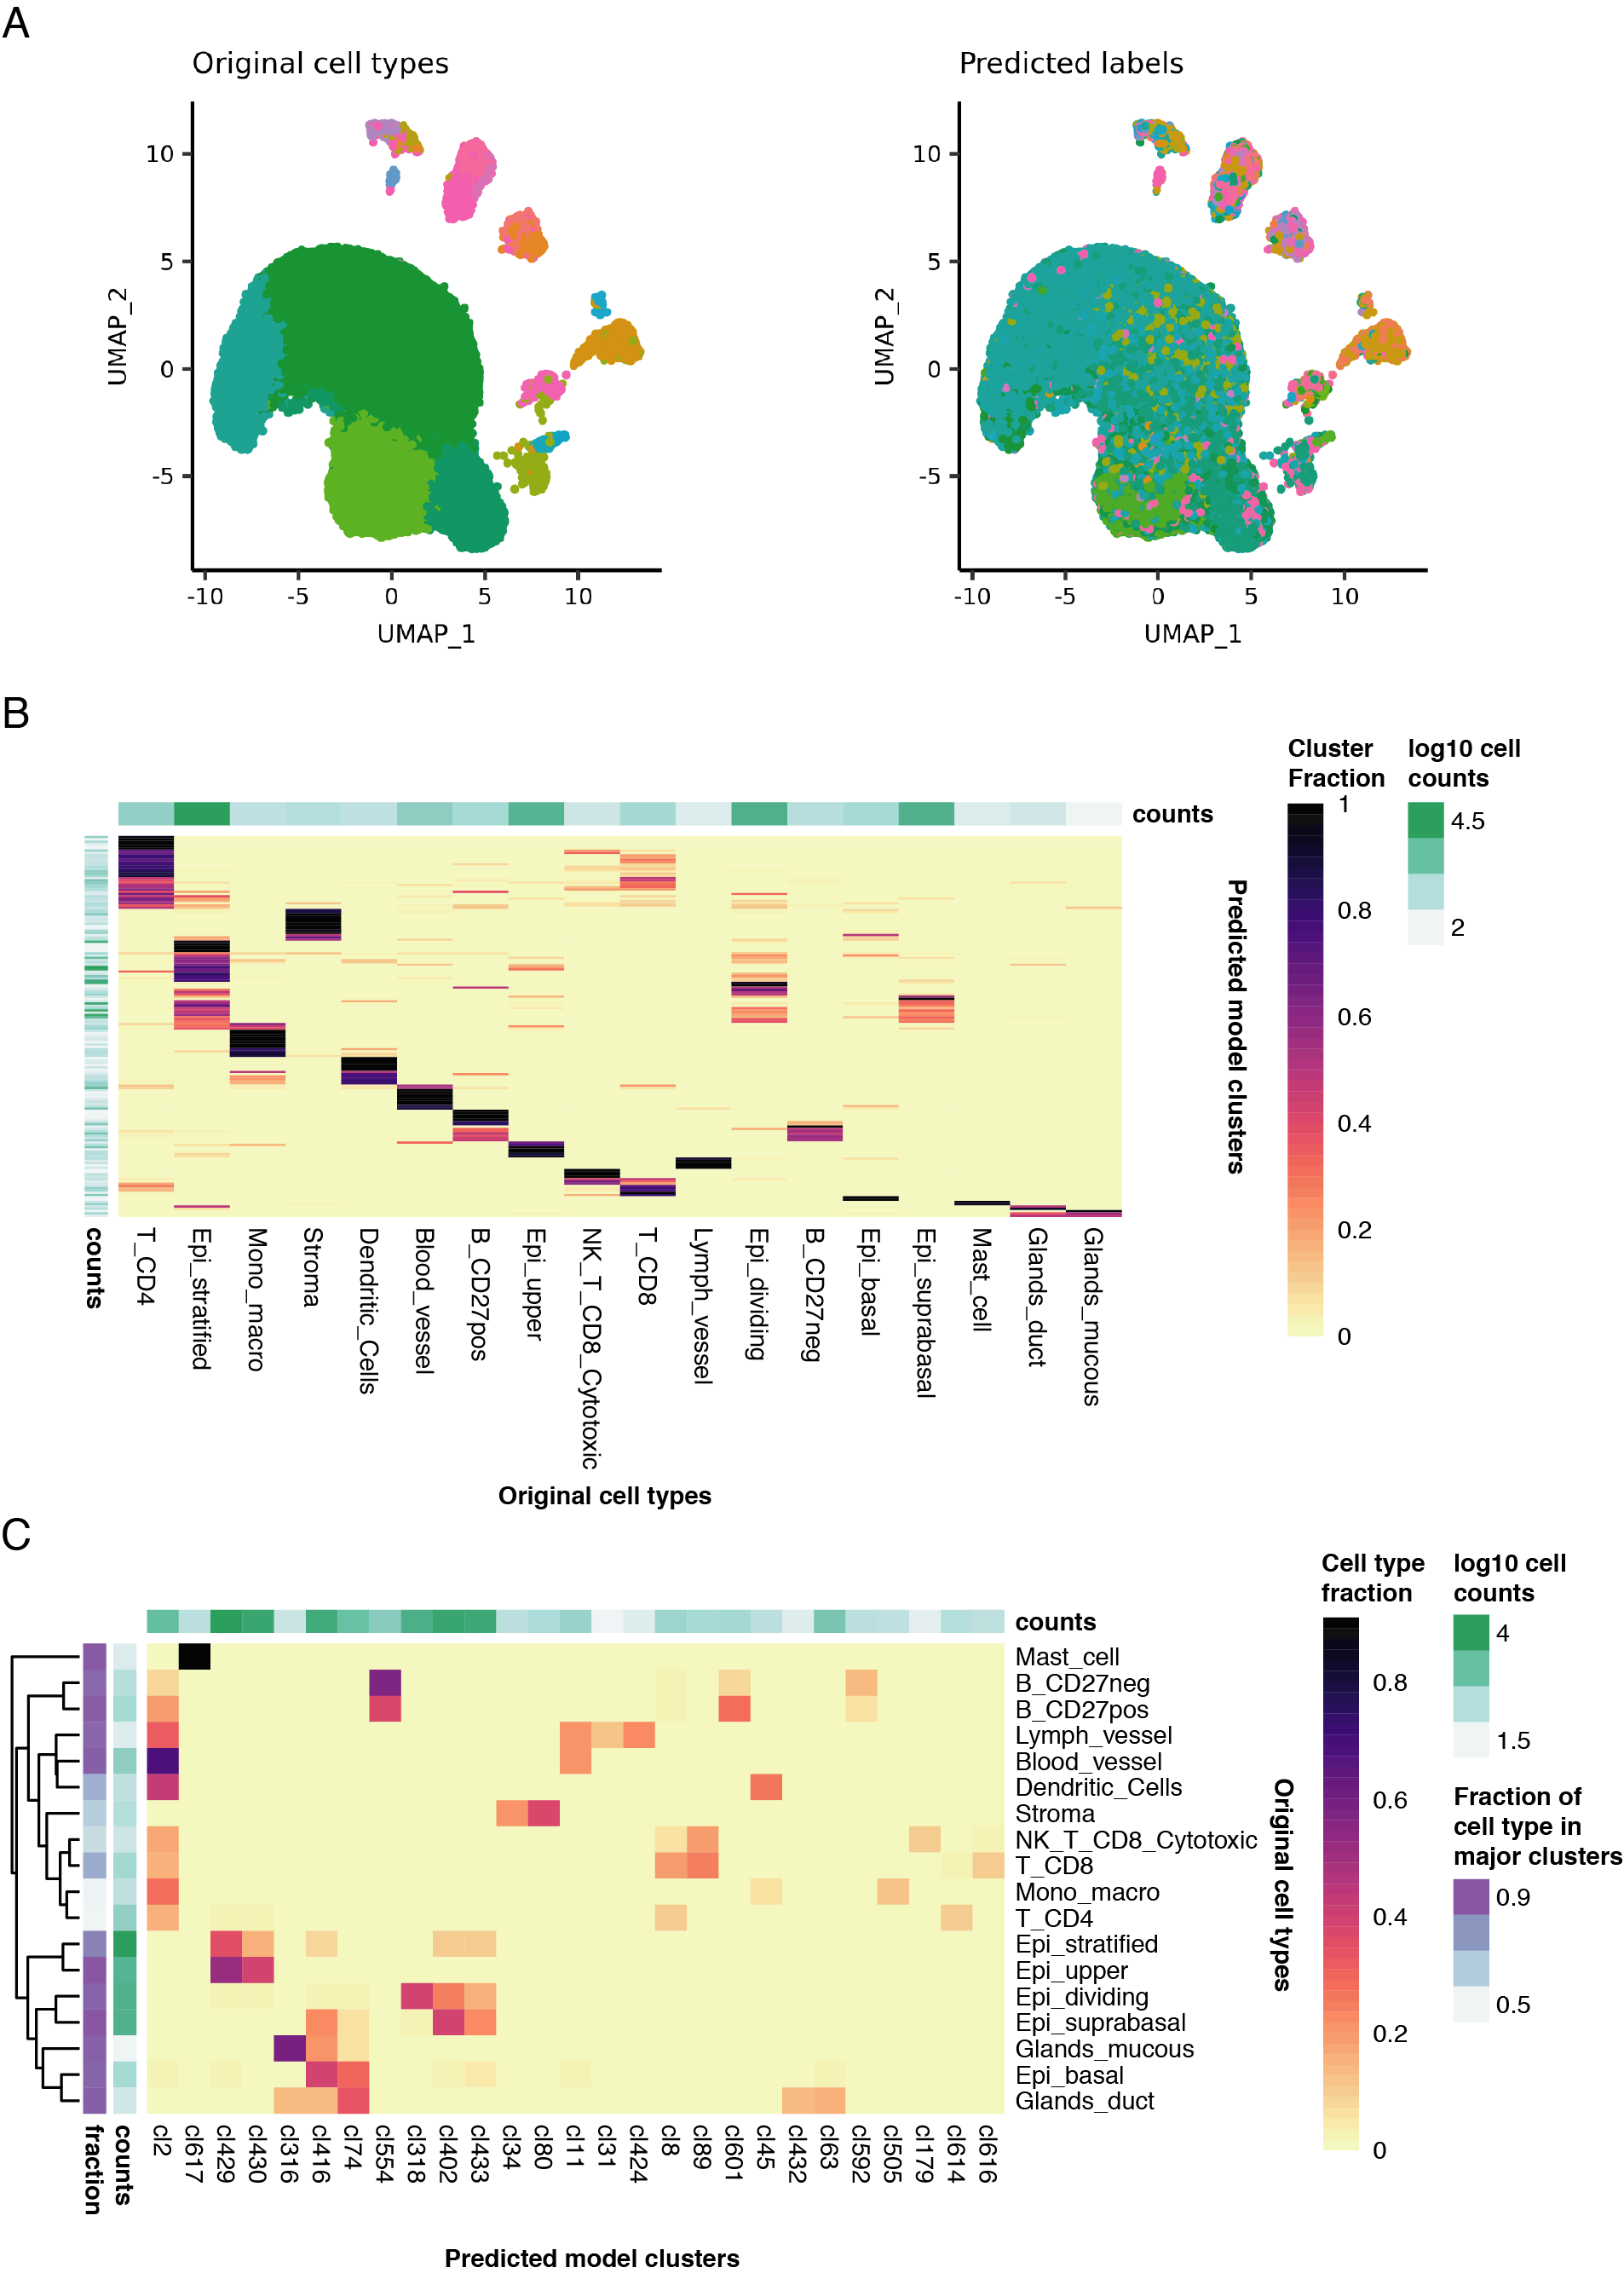
\includegraphics[scale=0.8]{Appendix3/Figs/appB_oes.png} % change word in curlies to change figure
\caption[\textit{CellTypist} predictions for oesophagus data from~\citep{madissoon_lung_2019}]{\textbf{\textit{CellTypist} predictions for oesophagus data from~\citep{madissoon_lung_2019} (Related to Figure~\ref{fig:chap4_preds})}\newline\textbf{(A)} UMAP projections coloured by the original cell type annotations (left) and those predicted by \textit{CellTypist} (right) using thr1 = 0.99 and thr2 = 0.8. \textbf{(B)} Proportion of clusters (rows) matching each annotated cell type (columns). \textbf{(C)} Proportion of annotated cell types (rows) included in each cluster (columns). Only clusters including at least 10\% of a given cell type were included.}
\label{fig:appB_oes}
\end{figure}


\begin{figure}[pht!] 
\centering
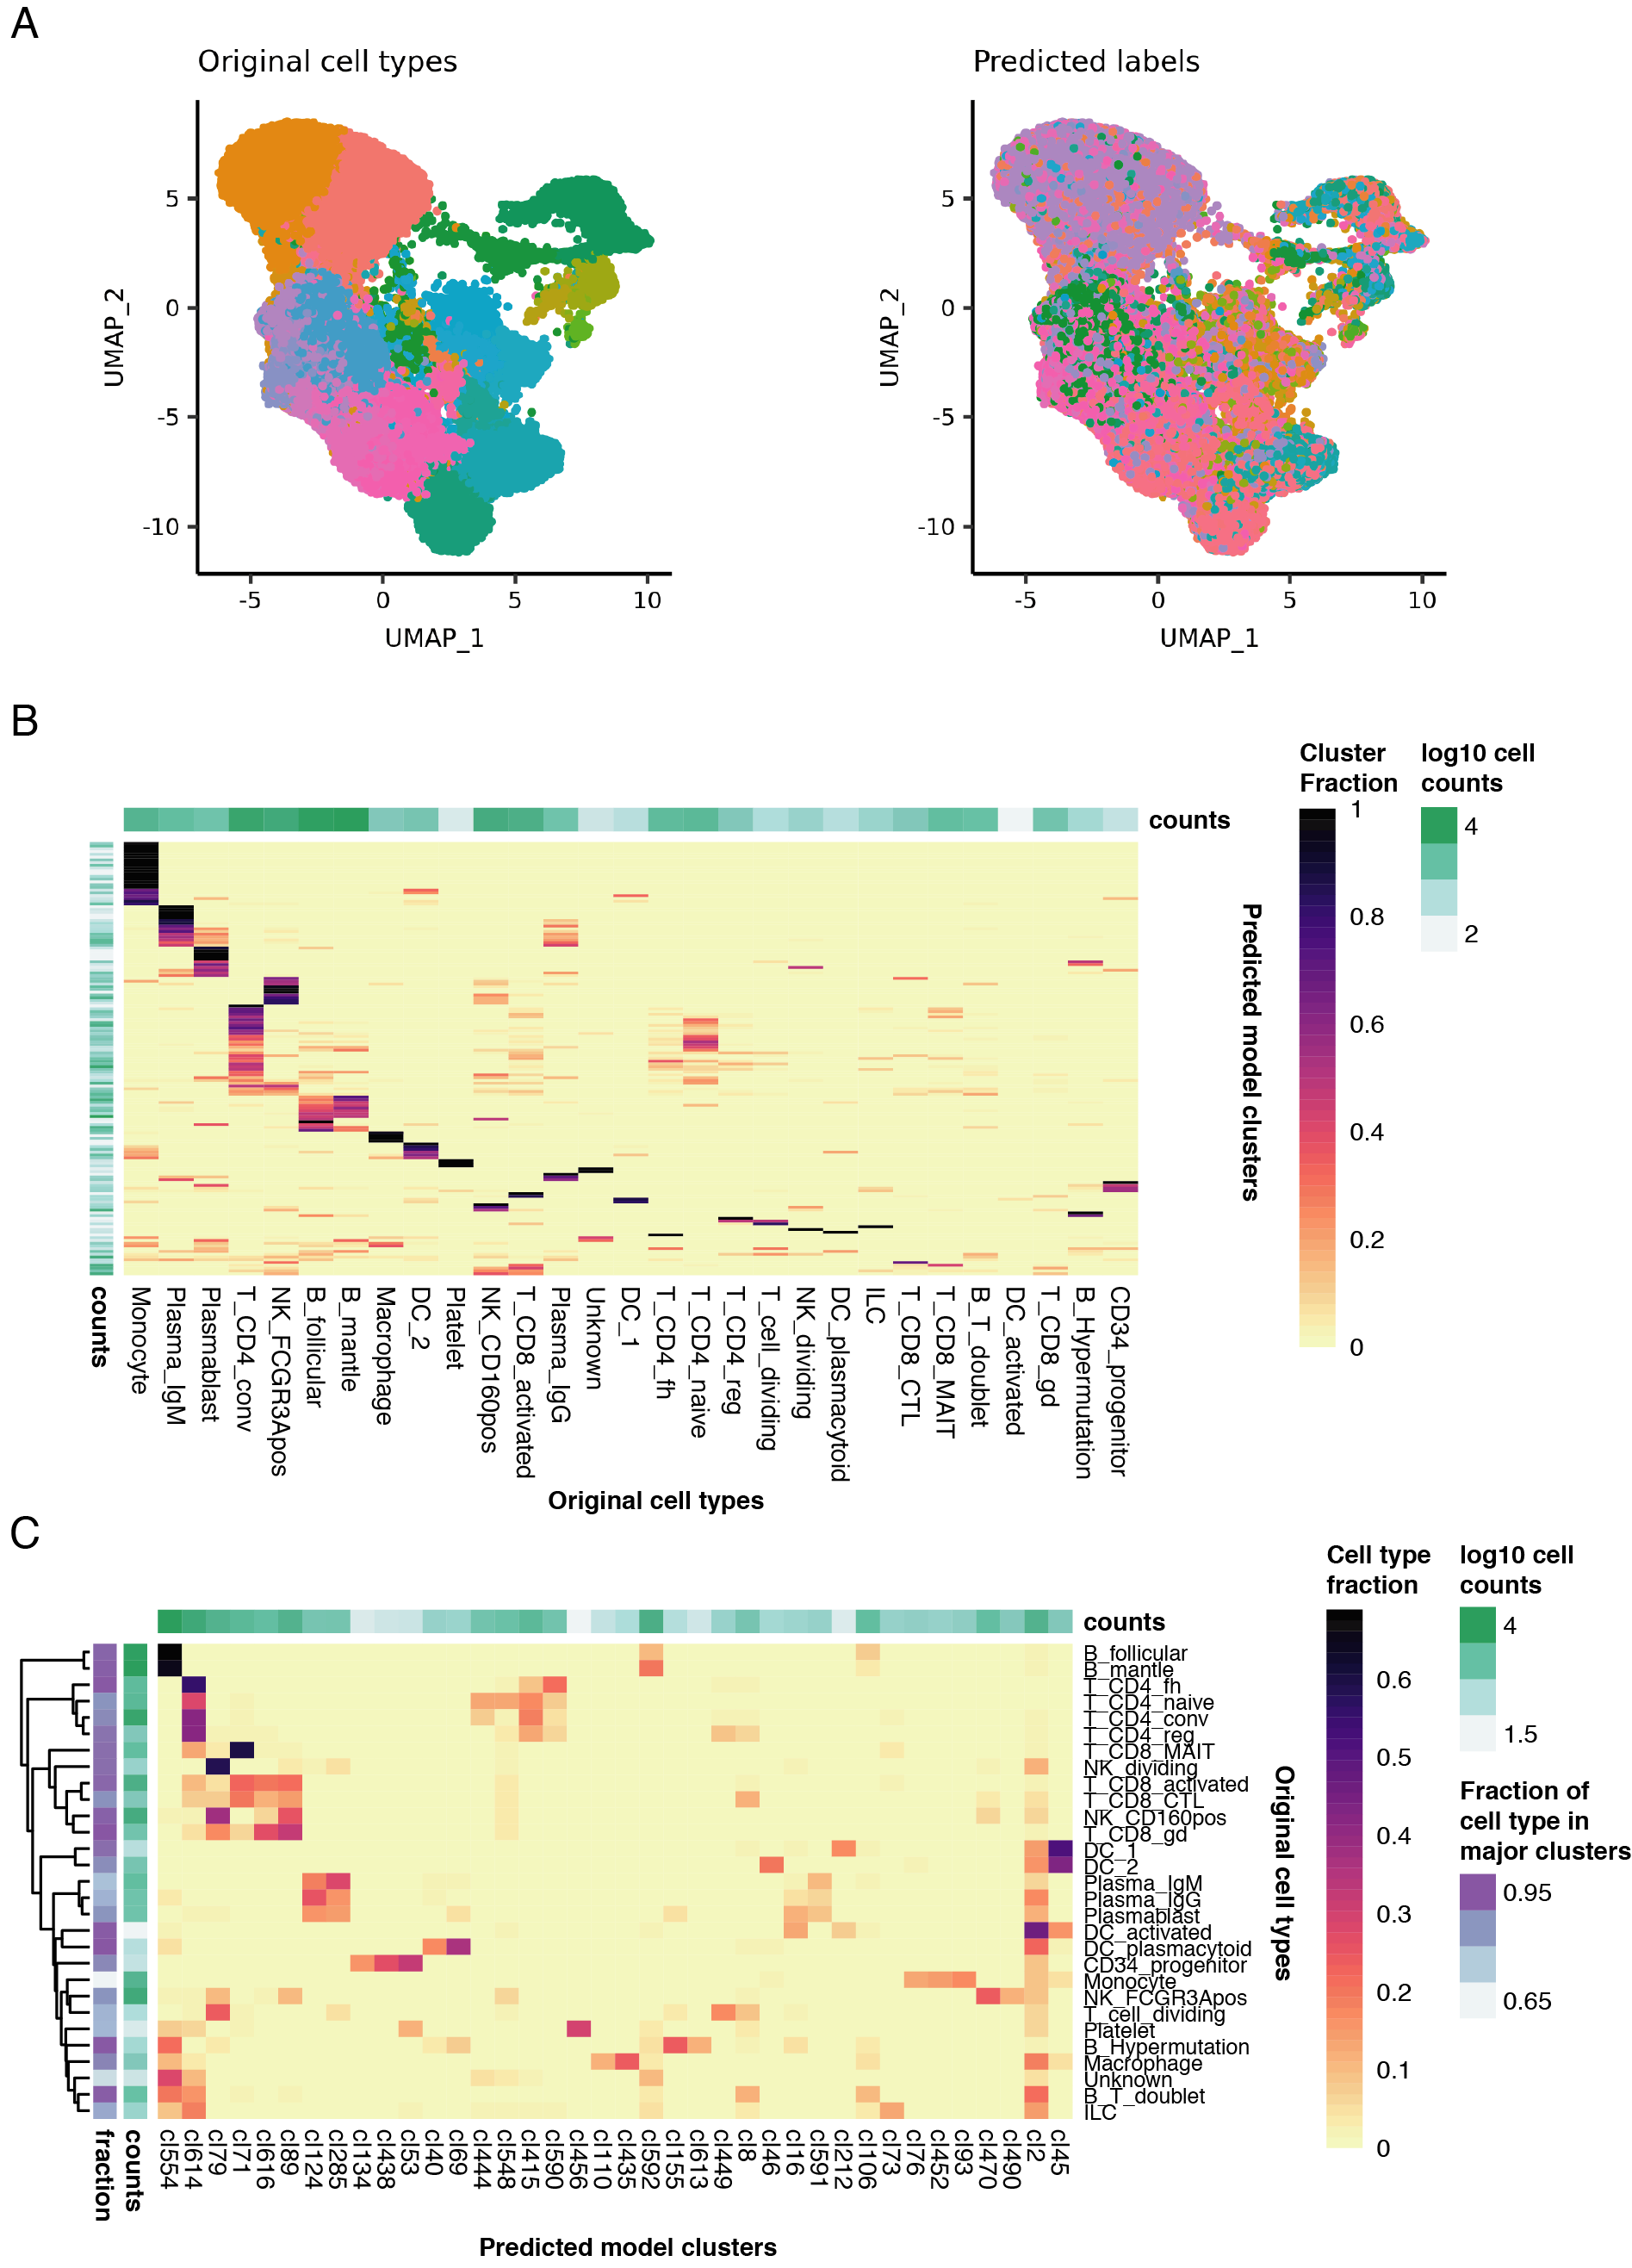
\includegraphics[scale=0.81]{Appendix3/Figs/appB_spleen.png} % change word in curlies to change figure
\caption[\textit{CellTypist} predictions for spleen data from~\citep{madissoon_lung_2019}]{\textbf{\textit{CellTypist} predictions for spleen data from~\citep{madissoon_lung_2019} (Related to Figure~\ref{fig:chap4_preds})}\newline\textbf{(A)} UMAP projections coloured by the original cell type annotations (left) and those predicted by \textit{CellTypist} (right) using thr1 = 0.99 and thr2 = 0.8. \textbf{(B)} Proportion of clusters (rows) matching each annotated cell type (columns). \textbf{(C)} Proportion of annotated cell types (rows) included in each cluster (columns). Only clusters including at least 10\% of a given cell type were included.}
\label{fig:appB_spleen}
\end{figure}


\begin{figure}[pht!] 
\centering
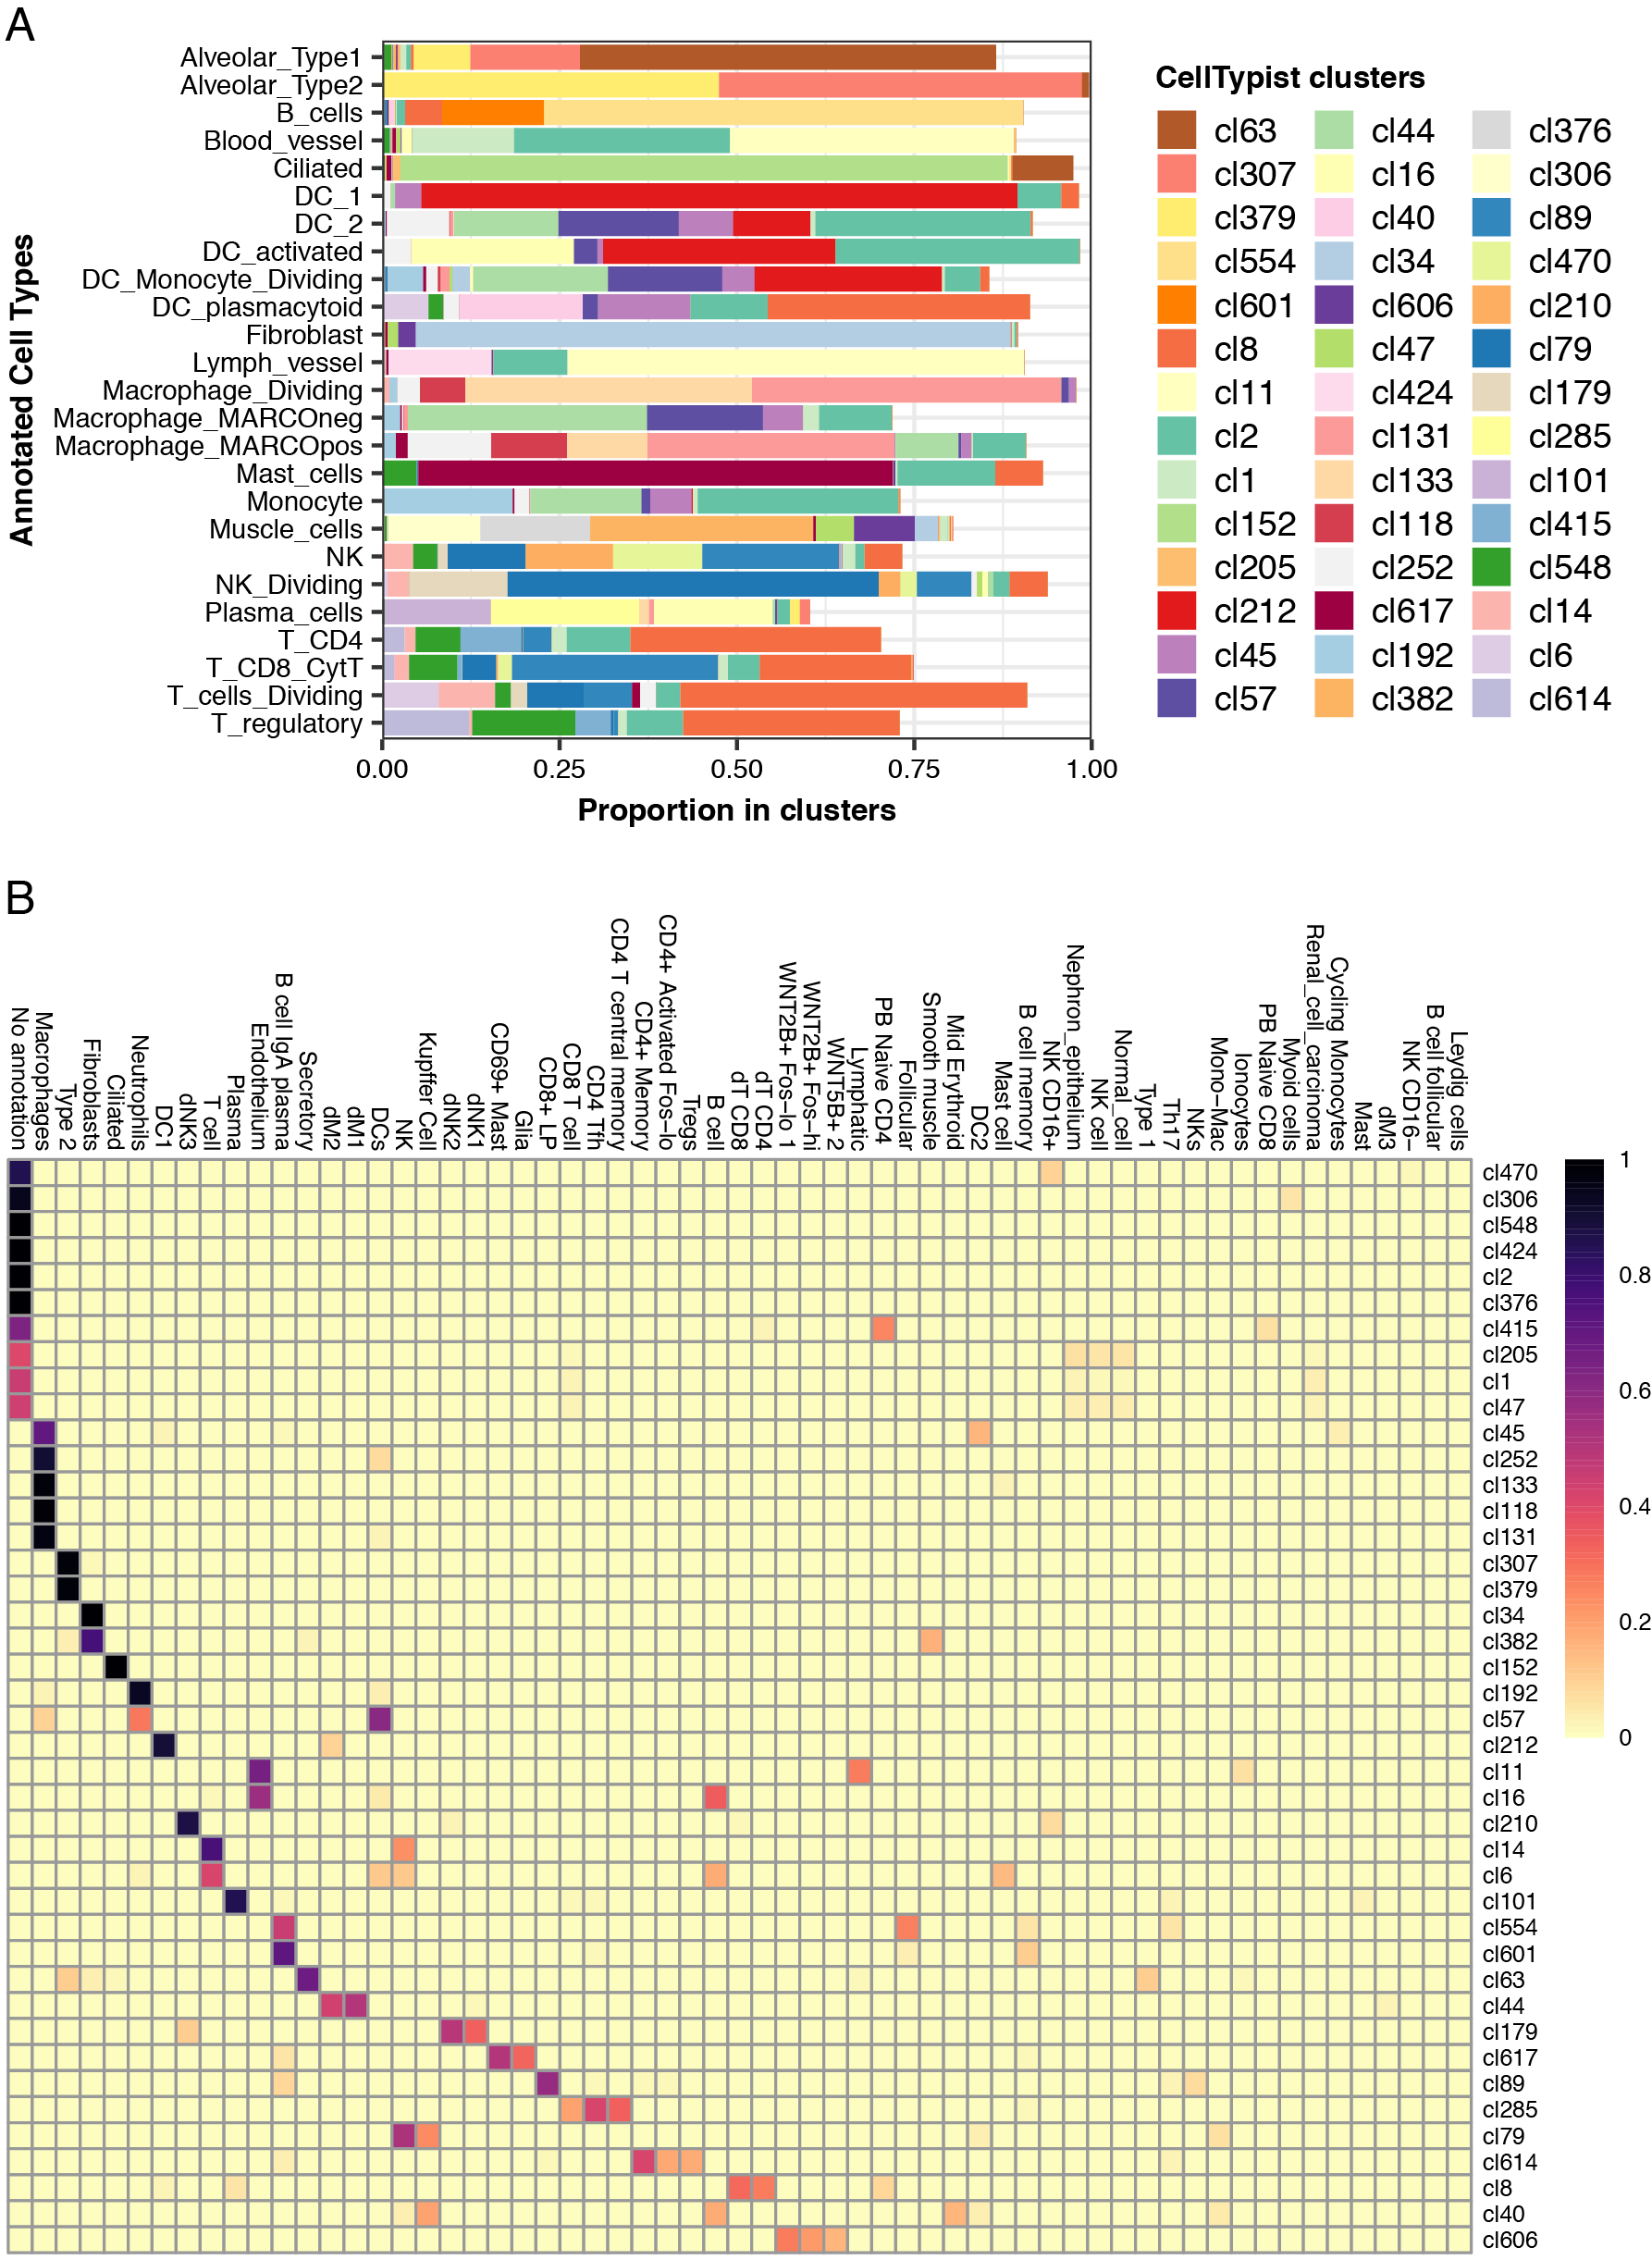
\includegraphics[scale=0.93]{Appendix3/Figs/appB_lung_labs_exp.png} % change word in curlies to change figure
\caption[Matching \textit{CellTypist} predictions in lung with annotations in the data collection]{\textbf{Matching \textit{CellTypist} predictions in lung with annotations in the data collection (Related to Figure~\ref{fig:chap4_preds})}\newline\textbf{(A)} \textit{CellTypist} clusters (thr1 = 0.99, thr2 = 0.8) matched to each original cell type annotation. Only the top 3 clusters per cell type were selected. \textbf{(B)} Proportion of cell type annotations (columns) represented in the \textit{CellTypist} clusters matched to lung.}
\label{fig:appB_lunglabs}
\end{figure}


\begin{figure}[ht!] 
\centering
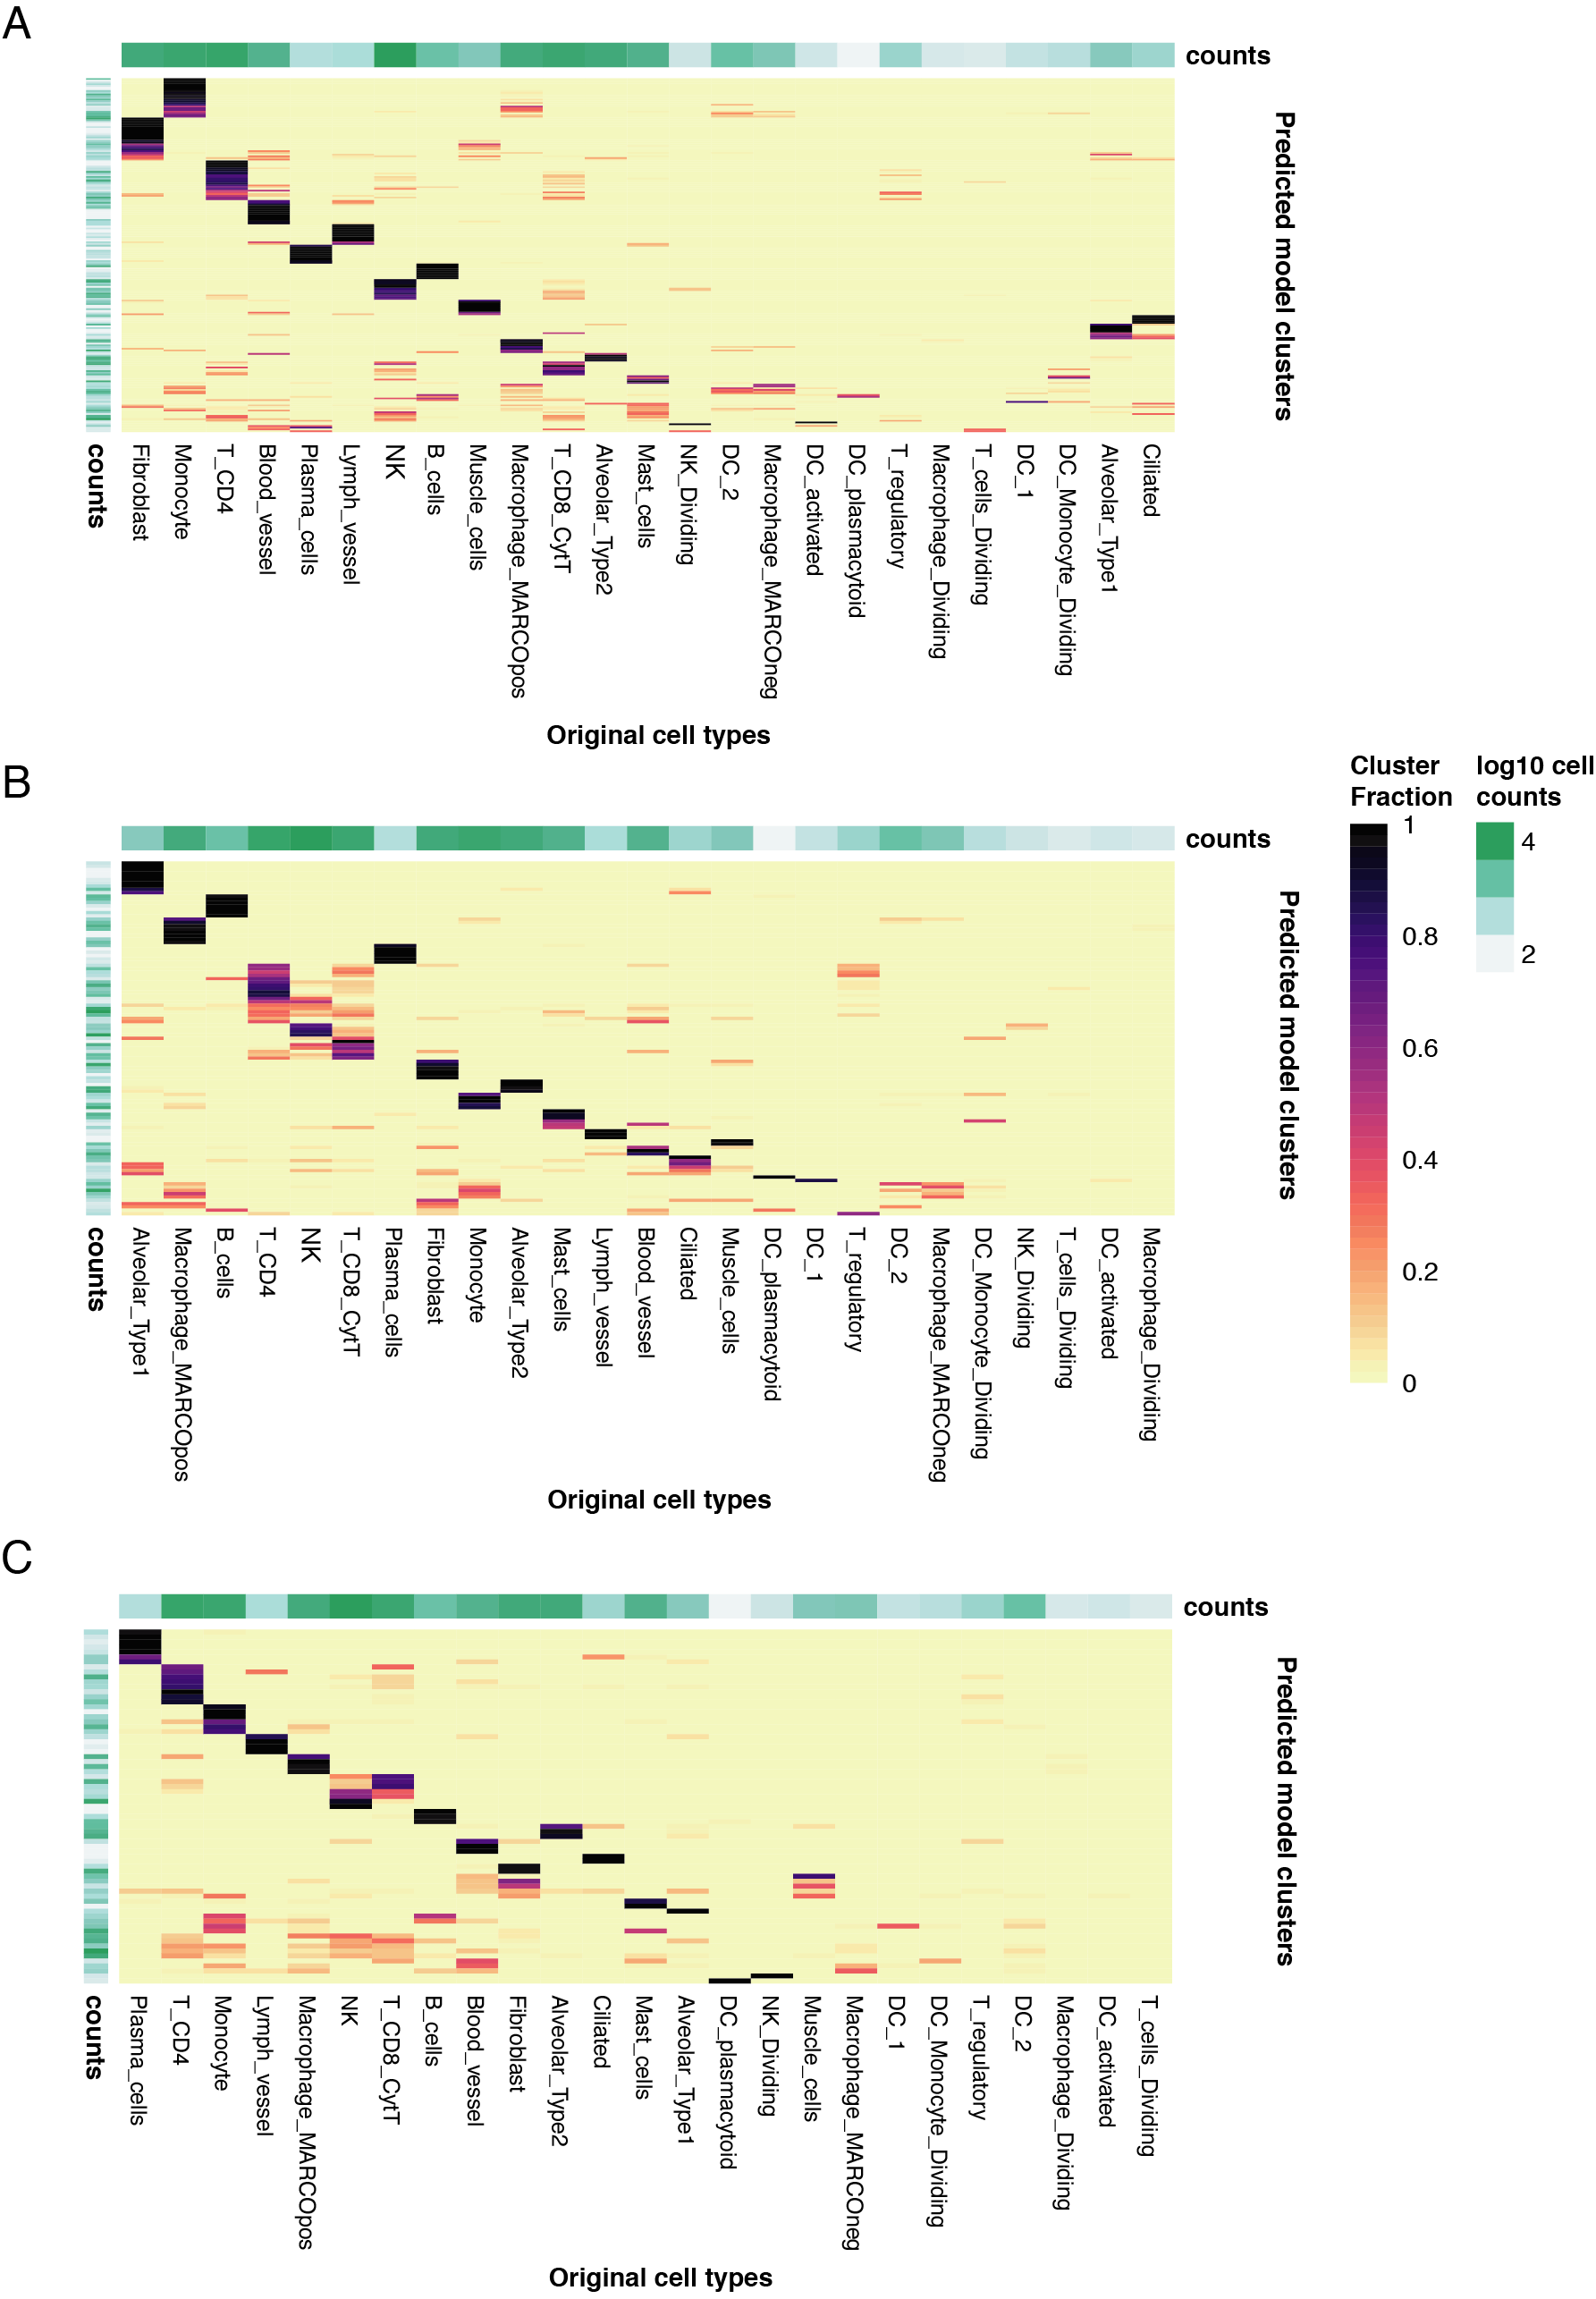
\includegraphics[scale=0.85]{Appendix3/Figs/appB_otherClustFrac_lung.png} % change word in curlies to change figure
\caption[Clusters matching lung annotated cell types in other \textit{CellTypist} models]{\textbf{Clusters matching lung annotated cell types in other \textit{CellTypist} models (Related to Figure~\ref{fig:chap4_preds}B)}\newline Proportion of clusters (rows) matching each annotated cell type (columns) in the models thr1 = 0.4, thr2 = 0.99 \textbf{(A)}, thr1 = 0.25, thr2 = 0.25 \textbf{(A)}, and thr1 = 0.1, thr2 = 0.1 \textbf{(C)}.}
\label{fig:appB_othercl}
\end{figure}


\begin{figure}[ht!] 
\centering
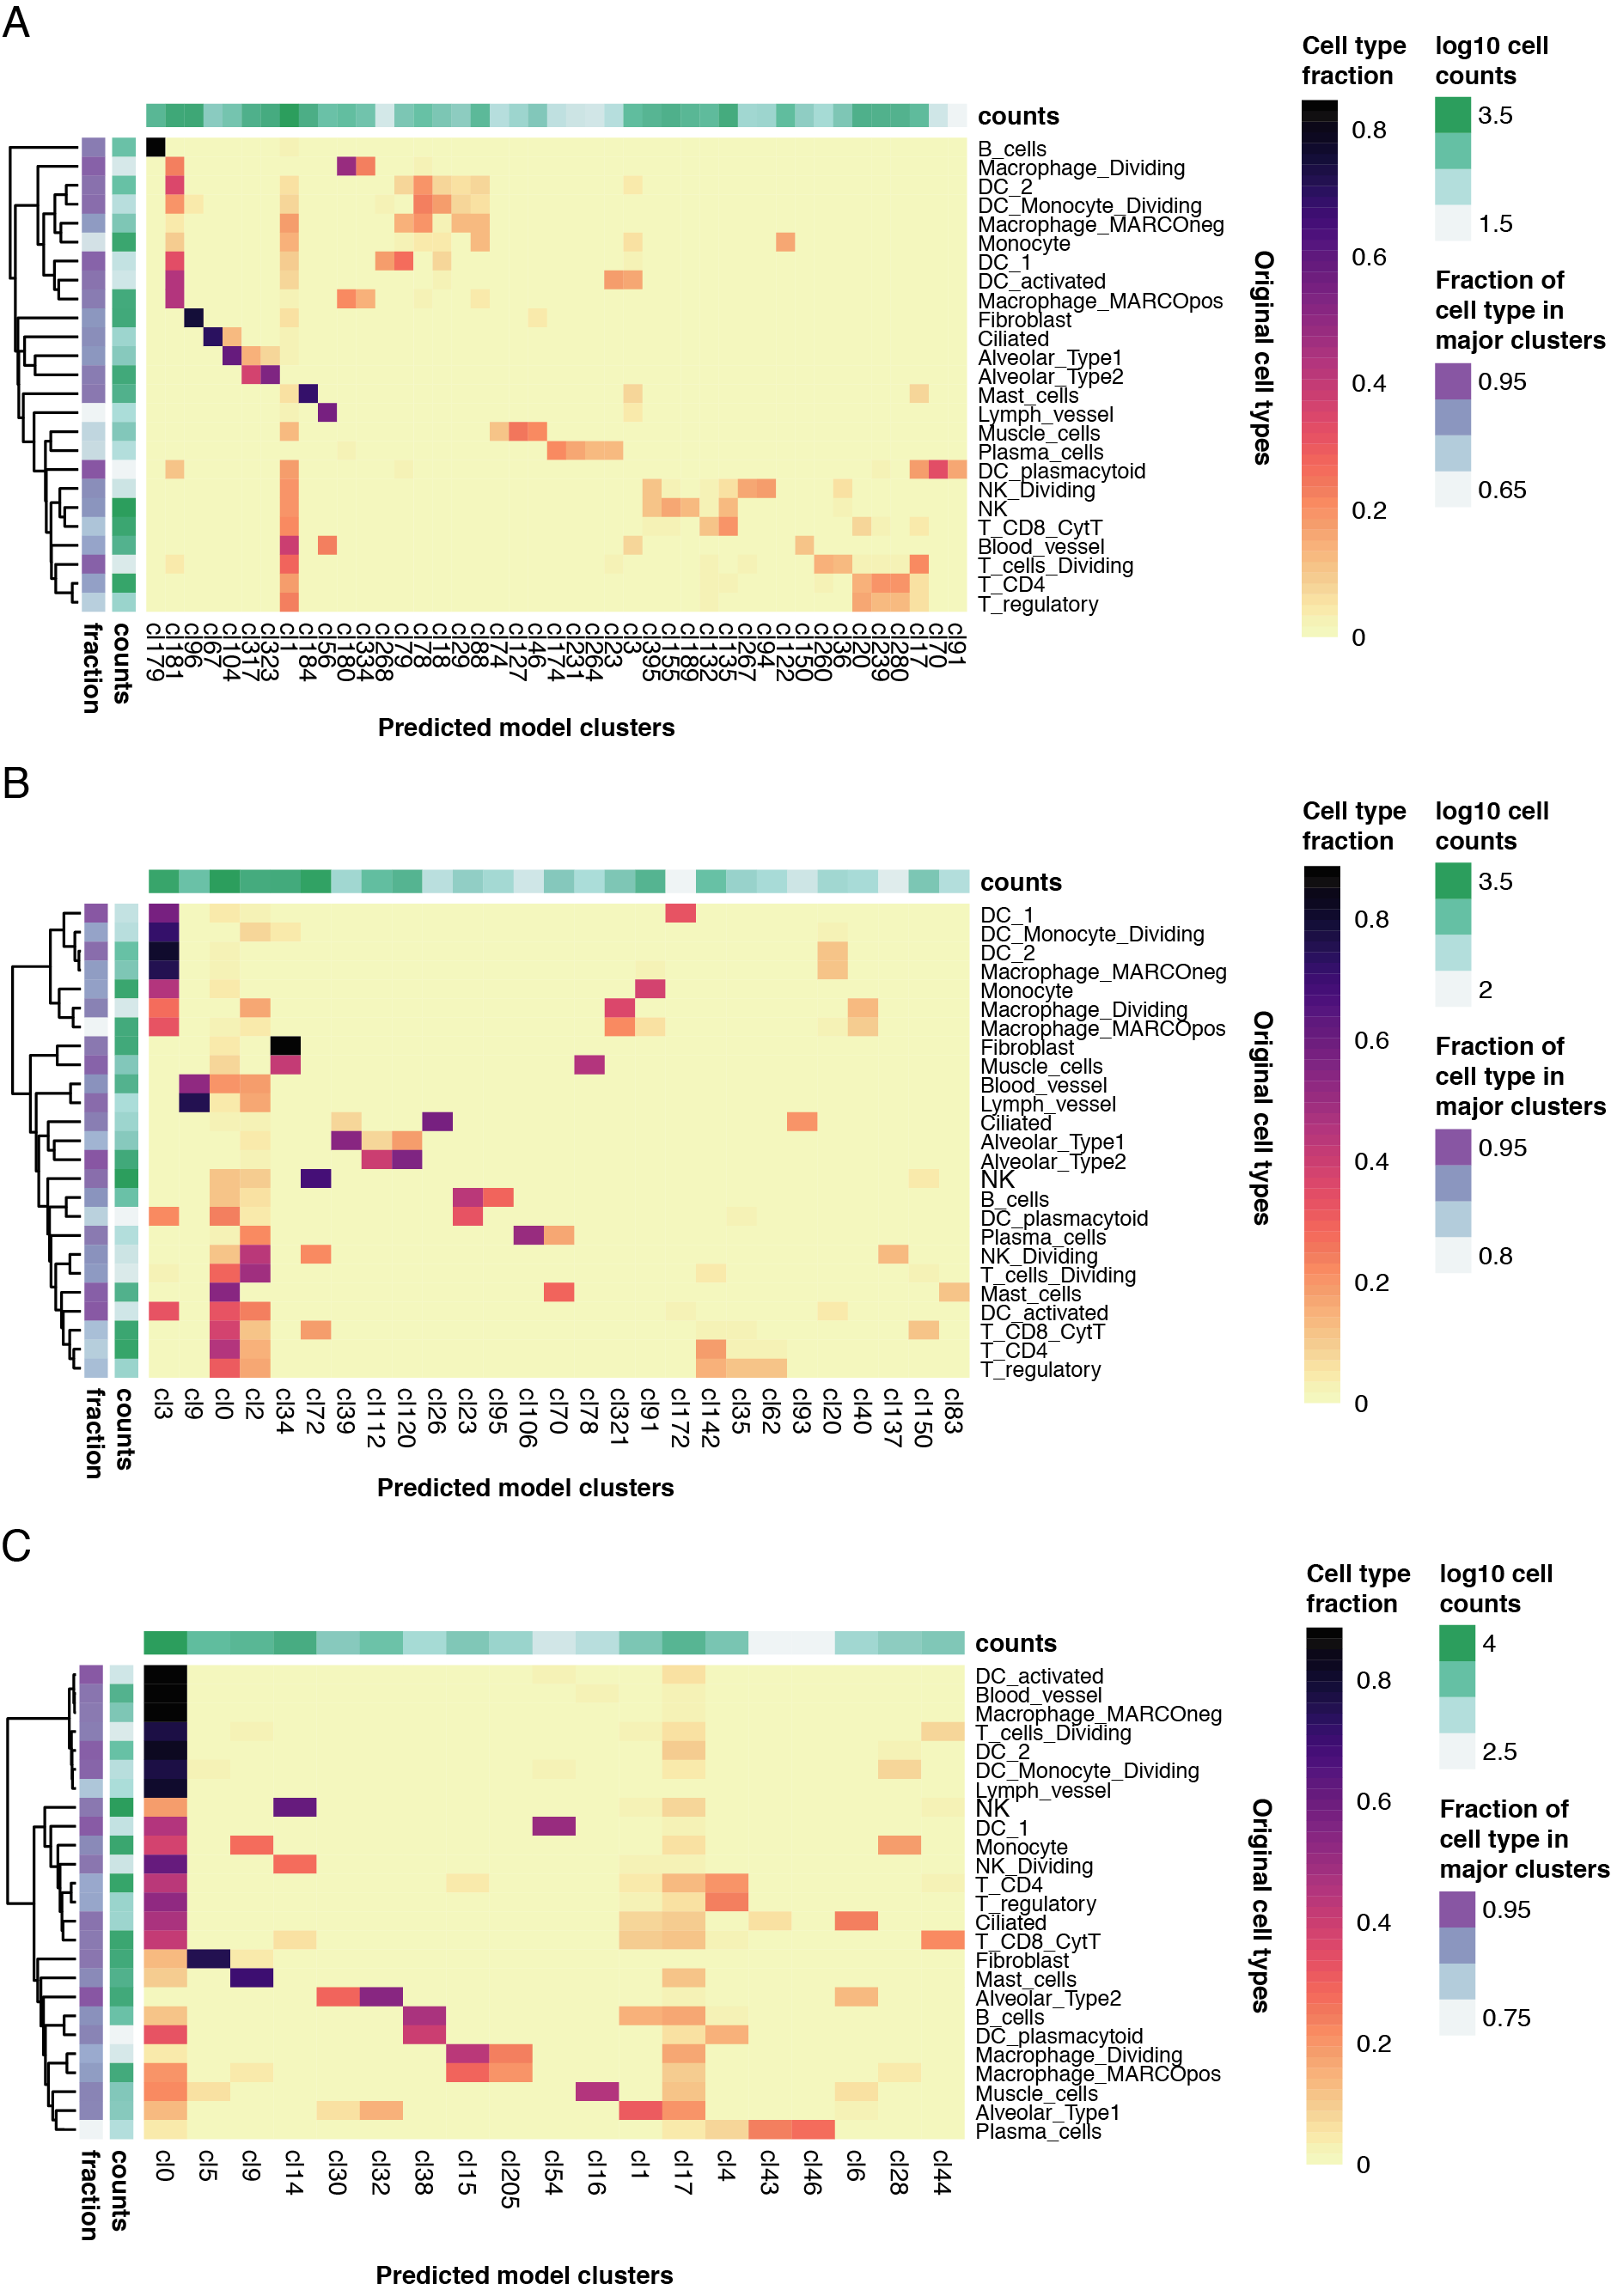
\includegraphics[scale=0.83]{Appendix3/Figs/appB_otherCtFrac_lung.png} % change word in curlies to change figure
\caption[Lung annotated cell types matching clusters in other \textit{CellTypist} models]{\textbf{Lung annotated cell types matching clusters in other \textit{CellTypist} models (Related to Figure~\ref{fig:chap4_preds}C)}\newline Proportion of annotated cell types (rows) included in each cluster (columns) in the models thr1 = 0.4, thr2 = 0.99 \textbf{(A)}, thr1 = 0.25, thr2 = 0.25 \textbf{(A)}, and thr1 = 0.1, thr2 = 0.1 \textbf{(C)}. Only clusters including at least 10\% of a given cell type were included.}
\label{fig:appB_otherct}
\end{figure}


\section{Supplementary Tables}
\label{sectionC1.2}

\begin{table}[pht!] % p for putting it in the next page available
\scriptsize
\caption[Cell types from~\citep{madissoon_lung_2019} with expression programmes enriched in \textit{CellTypist} clusters]{Cell types from~\citep{madissoon_lung_2019} with expression programmes enriched in \textit{CellTypist} clusters}
\centering
\label{table:tab_mad_match}
\begin{tabular}{lll}
  \toprule
Cluster & Tissue & Cell types \\ 
  \midrule
cl430 & Lung & Alveolar\_Type1 \\ 
  cl430 & Oesophagus & Epi\_upper,Epi\_stratified \\ 
  cl433 & Lung & Alveolar\_Type2 \\ 
  cl433 & Spleen & Plasmablast,DC\_1,Monocyte,NK\_dividing,Plasma\_IgG \\ 
  cl429 & Lung & Alveolar\_Type1 \\ 
  cl39 & Lung & T\_CD4,T\_cells\_Dividing,T\_regulatory \\ 
  cl39 & Spleen & T\_CD4\_fh,T\_CD4\_conv,T\_CD4\_reg,T\_CD8\_MAIT,T\_CD4\_naive \\ 
  cl39 & Oesophagus & T\_CD8,T\_CD4,NK\_T\_CD8\_Cytotoxic,Mast\_cell,Lymph\_vessel \\ 
  cl402 & Lung & Alveolar\_Type2,Alveolar\_Type1 \\ 
  cl402 & Oesophagus & Epi\_suprabasal \\ 
  cl318 & Lung & T\_cells\_Dividing,NK\_Dividing,DC\_Monocyte\_Dividing,Macrophage\_Dividing,Alveolar\_Type1 \\ 
  cl318 & Spleen & NK\_dividing,T\_cell\_dividing,B\_Hypermutation,Plasmablast,CD34\_progenitor \\ 
  cl318 & Oesophagus & Epi\_dividing \\ 
  cl416 & Lung & Alveolar\_Type1,Alveolar\_Type2,Ciliated,Lymph\_vessel \\ 
  cl416 & Oesophagus & Glands\_mucous,Epi\_basal,Glands\_duct,Epi\_suprabasal \\ 
  cl263 & Lung & Alveolar\_Type1,Alveolar\_Type2,Ciliated \\ 
  cl263 & Oesophagus & Epi\_stratified,Epi\_basal,Glands\_duct \\ 
  cl2 & Lung & DC\_2,DC\_activated,Lymph\_vessel,DC\_Monocyte\_Dividing,DC\_1 \\ 
  cl2 & Spleen & DC\_1,DC\_activated,DC\_2,DC\_plasmacytoid,T\_CD8\_gd \\ 
  cl2 & Oesophagus & Blood\_vessel,NK\_T\_CD8\_Cytotoxic,Mast\_cell,T\_CD8,Dendritic\_Cells \\ 
  cl1 & Lung & Blood\_vessel \\ 
  cl1 & Oesophagus & Blood\_vessel,Mast\_cell,Dendritic\_Cells,Stroma,NK\_T\_CD8\_Cytotoxic \\ 
  cl548 & Spleen & T\_CD8\_CTL,T\_CD8\_MAIT,T\_CD4\_conv \\ 
  cl548 & Oesophagus & T\_CD4,T\_CD8,NK\_T\_CD8\_Cytotoxic \\ 
  cl80 & Lung & Fibroblast,Muscle\_cells,Lymph\_vessel,Blood\_vessel \\ 
  cl80 & Spleen & T\_CD8\_MAIT,T\_CD8\_CTL \\ 
  cl80 & Oesophagus & Stroma,Epi\_basal,Lymph\_vessel,Glands\_duct,Epi\_suprabasal \\ 
  cl6 & Lung & T\_cells\_Dividing,DC\_Monocyte\_Dividing,DC\_1,DC\_activated,DC\_plasmacytoid \\ 
  cl6 & Spleen & T\_cell\_dividing,DC\_plasmacytoid,T\_CD8\_CTL,B\_Hypermutation,NK\_dividing \\ 
  cl6 & Oesophagus & Dendritic\_Cells,NK\_T\_CD8\_Cytotoxic,T\_CD8,T\_CD4,Mast\_cell \\ 
  cl614 & Lung & T\_CD4,T\_regulatory,T\_cells\_Dividing \\ 
  cl614 & Spleen & T\_CD4\_fh,T\_CD4\_reg,T\_CD4\_conv,T\_CD4\_naive \\ 
  cl614 & Oesophagus & T\_CD4,T\_CD8,NK\_T\_CD8\_Cytotoxic \\ 
  cl262 & Lung & Alveolar\_Type1,DC\_1,DC\_2,DC\_activated \\ 
  cl262 & Oesophagus & Epi\_stratified \\ 
  cl63 & Lung & Alveolar\_Type1,Alveolar\_Type2,Ciliated,Blood\_vessel,Lymph\_vessel \\ 
  cl63 & Spleen & DC\_activated,DC\_1,CD34\_progenitor,DC\_2,T\_CD8\_MAIT \\ 
  cl63 & Oesophagus & Glands\_duct,Epi\_basal,Glands\_mucous,Epi\_suprabasal,Lymph\_vessel \\ 
  cl513 & Lung & T\_CD4,T\_cells\_Dividing,T\_regulatory,Mast\_cells \\ 
  cl513 & Spleen & T\_CD4\_reg,T\_CD8\_MAIT,T\_CD4\_conv,T\_CD4\_fh,T\_cell\_dividing \\ 
  cl513 & Oesophagus & Mast\_cell,T\_CD4,NK\_T\_CD8\_Cytotoxic,T\_CD8 \\ 
  cl89 & Lung & NK\_Dividing,T\_CD8\_CytT,DC\_plasmacytoid,DC\_activated,NK \\ 
  cl89 & Spleen & T\_CD8\_activated,T\_CD8\_gd,T\_CD8\_MAIT,NK\_CD160pos,T\_CD8\_CTL \\ 
  cl89 & Oesophagus & NK\_T\_CD8\_Cytotoxic,T\_CD8,T\_CD4,B\_CD27pos,Mast\_cell \\ 
  cl377 & Lung & Alveolar\_Type2,Alveolar\_Type1 \\ 
  cl11 & Lung & Blood\_vessel,Lymph\_vessel,Muscle\_cells,Fibroblast,Alveolar\_Type2 \\ 
  cl11 & Spleen & B\_mantle,T\_cell\_dividing,NK\_dividing \\ 
  cl11 & Oesophagus & Blood\_vessel,Lymph\_vessel,Stroma,Epi\_basal \\ 
  cl424 & Lung & Lymph\_vessel,Blood\_vessel,Fibroblast \\ 
  cl424 & Oesophagus & Lymph\_vessel,Blood\_vessel \\ 
  cl329 & Lung & Ciliated,Mast\_cells,T\_CD4,Alveolar\_Type1,T\_CD8\_CytT \\ 
  cl329 & Spleen & T\_CD8\_gd,DC\_activated \\ 
  cl329 & Oesophagus & T\_CD4,T\_CD8,Glands\_duct,NK\_T\_CD8\_Cytotoxic,B\_CD27pos \\ 
  cl128 & Lung & Alveolar\_Type1,Alveolar\_Type2 \\ 
  cl128 & Oesophagus & Glands\_mucous,Epi\_stratified \\ 
  cl31 & Lung & Lymph\_vessel,Fibroblast,Alveolar\_Type1 \\ 
  cl31 & Spleen & DC\_activated,T\_CD4\_naive \\ 
  cl31 & Oesophagus & Lymph\_vessel,Epi\_basal \\ 
  cl8 & Lung & T\_cells\_Dividing,T\_CD4,T\_CD8\_CytT,T\_regulatory,DC\_plasmacytoid \\ 
  cl8 & Spleen & T\_CD4\_reg,T\_CD4\_conv,T\_CD8\_activated,T\_cell\_dividing,T\_CD8\_CTL \\ 
  cl8 & Oesophagus & T\_CD4,T\_CD8,NK\_T\_CD8\_Cytotoxic,Mast\_cell,B\_CD27neg \\ 
   \bottomrule
\end{tabular}
\end{table}  
  
\begin{table}[pht!] % p for putting it in the next page available
\scriptsize
\caption[Cell types from~\citep{madissoon_lung_2019} with expression programmes enriched in \textit{CellTypist} clusters (continued 1)]{Cell types from~\citep{madissoon_lung_2019} with expression programmes enriched in \textit{CellTypist} clusters (continued 1)}
\centering
\label{table:tab_mad_match1}
\begin{tabular}{lll}
  \toprule
Cluster & Tissue & Cell types \\ 
  \midrule
cl554 & Lung & B\_cells,DC\_plasmacytoid,DC\_activated,T\_cells\_Dividing \\ 
  cl554 & Spleen & B\_follicular,B\_mantle,B\_Hypermutation \\ 
  cl554 & Oesophagus & B\_CD27pos,B\_CD27neg,T\_CD4,Dendritic\_Cells,NK\_T\_CD8\_Cytotoxic \\ 
  cl425 & Lung & Lymph\_vessel,Blood\_vessel,Muscle\_cells,Fibroblast \\ 
  cl425 & Spleen & DC\_1 \\ 
  cl425 & Oesophagus & Lymph\_vessel,Blood\_vessel,Stroma,Epi\_basal,Glands\_duct \\ 
  cl210 & Lung & NK\_Dividing,NK,T\_cells\_Dividing,DC\_plasmacytoid,DC\_1 \\ 
  cl210 & Spleen & NK\_CD160pos,NK\_FCGR3Apos,T\_CD8\_gd,NK\_dividing,T\_CD8\_MAIT \\ 
  cl210 & Oesophagus & NK\_T\_CD8\_Cytotoxic,T\_CD8,T\_CD4,Dendritic\_Cells,B\_CD27pos \\ 
  cl87 & Lung & T\_CD4 \\ 
  cl87 & Spleen & T\_CD8\_MAIT,Monocyte \\ 
  cl87 & Oesophagus & T\_CD4,T\_CD8,NK\_T\_CD8\_Cytotoxic,Mast\_cell \\ 
  cl47 & Lung & Fibroblast,Muscle\_cells,NK\_Dividing,Blood\_vessel,Lymph\_vessel \\ 
  cl47 & Oesophagus & Stroma,Blood\_vessel,Epi\_basal,Lymph\_vessel \\ 
  cl222 & Lung & Lymph\_vessel,Blood\_vessel,Fibroblast \\ 
  cl222 & Oesophagus & Lymph\_vessel,Blood\_vessel,Stroma \\ 
  cl88 & Lung & Blood\_vessel,Lymph\_vessel,Alveolar\_Type1,DC\_activated,Muscle\_cells \\ 
  cl88 & Spleen & T\_CD8\_MAIT,T\_CD4\_conv,T\_CD4\_naive,DC\_activated \\ 
  cl88 & Oesophagus & Blood\_vessel,Lymph\_vessel,Epi\_basal,Glands\_duct,Stroma \\ 
  cl73 & Lung & T\_cells\_Dividing,T\_CD4,T\_regulatory,DC\_activated \\ 
  cl73 & Spleen & T\_CD4\_reg,T\_CD8\_MAIT,ILC,T\_CD4\_fh,T\_CD4\_conv \\ 
  cl73 & Oesophagus & T\_CD4,T\_CD8,NK\_T\_CD8\_Cytotoxic,Mast\_cell,B\_CD27pos \\ 
  cl606 & Lung & Fibroblast,Muscle\_cells,DC\_activated,Macrophage\_MARCOpos,Macrophage\_MARCOneg \\ 
  cl606 & Spleen & Monocyte,DC\_1,DC\_2,Macrophage \\ 
  cl606 & Oesophagus & Stroma,Mast\_cell,Epi\_suprabasal,Mono\_macro,Lymph\_vessel \\ 
  cl449 & Spleen & T\_cell\_dividing,T\_CD4\_conv,T\_CD4\_fh,B\_Hypermutation,CD34\_progenitor \\ 
  cl449 & Oesophagus & Lymph\_vessel,Blood\_vessel,Glands\_duct \\ 
  cl58 & Lung & T\_regulatory,T\_cells\_Dividing,T\_CD4,T\_CD8\_CytT,Mast\_cells \\ 
  cl58 & Spleen & NK\_CD160pos,T\_CD4\_reg,T\_CD8\_gd,T\_CD8\_MAIT,T\_CD8\_CTL \\ 
  cl58 & Oesophagus & T\_CD8,T\_CD4,NK\_T\_CD8\_Cytotoxic,Mast\_cell,Dendritic\_Cells \\ 
  cl74 & Lung & Alveolar\_Type1 \\ 
  cl74 & Oesophagus & Epi\_basal,Glands\_duct \\ 
  cl147 & Spleen & CD34\_progenitor \\ 
  cl71 & Lung & T\_CD8\_CytT \\ 
  cl71 & Spleen & T\_CD8\_MAIT,T\_CD8\_activated,T\_CD8\_CTL,T\_CD8\_gd \\ 
  cl71 & Oesophagus & T\_CD4,T\_CD8 \\ 
  cl616 & Lung & T\_CD8\_CytT,NK\_Dividing,NK,T\_regulatory,T\_cells\_Dividing \\ 
  cl616 & Spleen & T\_CD8\_activated,T\_CD8\_MAIT,T\_CD8\_gd,NK\_CD160pos,T\_CD4\_fh \\ 
  cl616 & Oesophagus & T\_CD8,NK\_T\_CD8\_Cytotoxic,T\_CD4 \\ 
  cl179 & Lung & NK\_Dividing,NK,T\_cells\_Dividing \\ 
  cl179 & Spleen & NK\_dividing,NK\_CD160pos,T\_CD8\_gd,NK\_FCGR3Apos,ILC \\ 
  cl179 & Oesophagus & NK\_T\_CD8\_Cytotoxic,T\_CD8,Epi\_dividing,T\_CD4,Mast\_cell \\ 
  cl34 & Lung & Fibroblast,Muscle\_cells,Monocyte \\ 
  cl34 & Spleen & Monocyte,T\_CD8\_CTL \\ 
  cl34 & Oesophagus & Stroma,Lymph\_vessel,Dendritic\_Cells,Epi\_basal,Mono\_macro \\ 
  cl271 & Lung & Fibroblast,Muscle\_cells,Lymph\_vessel,Blood\_vessel \\ 
  cl271 & Oesophagus & Stroma,Lymph\_vessel,Epi\_basal,Blood\_vessel,Epi\_suprabasal \\ 
  cl172 & Lung & Lymph\_vessel,Blood\_vessel,Fibroblast \\ 
  cl172 & Oesophagus & Lymph\_vessel,Blood\_vessel,Stroma,Epi\_basal,Epi\_suprabasal \\ 
  cl435 & Lung & Macrophage\_MARCOneg,Macrophage\_MARCOpos \\ 
  cl435 & Spleen & Macrophage,DC\_2,Monocyte \\ 
  cl79 & Lung & NK\_Dividing,NK,T\_CD8\_CytT,T\_cells\_Dividing,T\_regulatory \\ 
  cl79 & Spleen & T\_CD8\_activated,NK\_dividing,T\_CD8\_gd,T\_CD8\_CTL,NK\_CD160pos \\ 
  cl79 & Oesophagus & NK\_T\_CD8\_Cytotoxic,T\_CD8,T\_CD4,Epi\_dividing,Mono\_macro \\ 
  cl36 & Lung & Blood\_vessel,DC\_activated,DC\_Monocyte\_Dividing,DC\_plasmacytoid,Macrophage\_MARCOpos \\ 
  cl36 & Spleen & DC\_2,DC\_activated,DC\_1,B\_follicular,Macrophage \\ 
  cl36 & Oesophagus & Blood\_vessel,Dendritic\_Cells,Mono\_macro,B\_CD27pos,B\_CD27neg \\ 
  cl505 & Spleen & Monocyte \\ 
  cl404 & Lung & Muscle\_cells,Fibroblast \\ 
  cl404 & Oesophagus & Epi\_suprabasal \\ 
   \bottomrule
\end{tabular}
\end{table}  
  
\begin{table}[pht!] % p for putting it in the next page available
\scriptsize
\caption[Cell types from~\citep{madissoon_lung_2019} with expression programmes enriched in \textit{CellTypist} clusters (continued 2)]{Cell types from~\citep{madissoon_lung_2019} with expression programmes enriched in \textit{CellTypist} clusters (continued 2)}
\centering
\label{table:tab_mad_match2}
\begin{tabular}{lll}
  \toprule
Cluster & Tissue & Cell types \\ 
  \midrule
  cl464 & Lung & Macrophage\_MARCOneg \\ 
  cl464 & Spleen & CD34\_progenitor,DC\_2 \\ 
  cl464 & Oesophagus & Dendritic\_Cells \\ 
  cl596 & Lung & T\_CD4,T\_cells\_Dividing,T\_regulatory,Mast\_cells,B\_cells \\ 
  cl596 & Spleen & T\_CD8\_MAIT,T\_CD4\_conv,T\_CD4\_fh,T\_CD4\_reg,T\_CD4\_naive \\ 
  cl596 & Oesophagus & T\_CD8,NK\_T\_CD8\_Cytotoxic,T\_CD4,Dendritic\_Cells,B\_CD27pos \\ 
  cl45 & Lung & DC\_2,Macrophage\_MARCOneg,DC\_1,DC\_Monocyte\_Dividing,DC\_plasmacytoid \\ 
  cl45 & Spleen & DC\_2,DC\_1,DC\_activated,DC\_plasmacytoid,Monocyte \\ 
  cl45 & Oesophagus & Dendritic\_Cells,Mono\_macro,B\_CD27pos,B\_CD27neg,Blood\_vessel \\ 
  cl51 & Lung & DC\_2,Macrophage\_MARCOneg,DC\_1,DC\_activated,DC\_Monocyte\_Dividing \\ 
  cl51 & Spleen & DC\_2,DC\_1,DC\_activated,Monocyte,Macrophage \\ 
  cl51 & Oesophagus & Dendritic\_Cells,Mono\_macro,T\_CD4,B\_CD27pos,B\_CD27neg \\ 
  cl441 & Spleen & T\_CD4\_naive \\ 
  cl432 & Lung & Alveolar\_Type1,Ciliated,Alveolar\_Type2 \\ 
  cl432 & Spleen & B\_mantle \\ 
  cl432 & Oesophagus & Glands\_duct,Glands\_mucous,Epi\_basal \\ 
  cl617 & Lung & DC\_2,Mast\_cells,Muscle\_cells \\ 
  cl617 & Spleen & Monocyte,T\_CD8\_MAIT \\ 
  cl617 & Oesophagus & Mast\_cell,Dendritic\_Cells,Epi\_basal,B\_CD27pos,Mono\_macro \\ 
  cl260 & Lung & DC\_plasmacytoid,Alveolar\_Type1,Ciliated,Monocyte,DC\_activated \\ 
  cl260 & Spleen & CD34\_progenitor \\ 
  cl260 & Oesophagus & Blood\_vessel,Epi\_suprabasal \\ 
  cl452 & Lung & Monocyte \\ 
  cl452 & Spleen & Monocyte \\ 
  cl27 & Lung & Blood\_vessel,Lymph\_vessel,Muscle\_cells \\ 
  cl27 & Oesophagus & Blood\_vessel,Lymph\_vessel,Stroma \\ 
  cl64 & Lung & Blood\_vessel,Lymph\_vessel,Fibroblast,Muscle\_cells \\ 
  cl64 & Spleen & T\_CD4\_conv \\ 
  cl64 & Oesophagus & Blood\_vessel,Lymph\_vessel,Stroma,Epi\_basal \\ 
  cl205 & Lung & T\_CD8\_CytT \\ 
  cl205 & Spleen & T\_CD8\_gd,T\_CD8\_CTL \\ 
  cl252 & Lung & Macrophage\_MARCOpos,Macrophage\_Dividing,DC\_activated,DC\_Monocyte\_Dividing,DC\_2 \\ 
  cl252 & Spleen & DC\_2,DC\_1,NK\_dividing,DC\_activated,CD34\_progenitor \\ 
  cl252 & Oesophagus & NK\_T\_CD8\_Cytotoxic,T\_CD4,Mast\_cell,Mono\_macro,T\_CD8 \\ 
  cl76 & Spleen & Monocyte \\ 
  cl508 & Lung & T\_CD8\_CytT,T\_CD4,T\_regulatory,NK,NK\_Dividing \\ 
  cl508 & Spleen & T\_CD8\_CTL,T\_CD8\_MAIT,T\_CD8\_activated,T\_CD8\_gd,T\_CD4\_fh \\ 
  cl508 & Oesophagus & T\_CD8,T\_CD4,NK\_T\_CD8\_Cytotoxic \\ 
  cl621 & Lung & T\_cells\_Dividing,T\_CD4,T\_regulatory,DC\_activated \\ 
  cl621 & Spleen & T\_CD8\_MAIT,T\_CD4\_reg,T\_cell\_dividing,Monocyte,T\_CD4\_conv \\ 
  cl621 & Oesophagus & T\_CD4,T\_CD8,Dendritic\_Cells,NK\_T\_CD8\_Cytotoxic,Mast\_cell \\ 
  cl512 & Lung & Monocyte,Macrophage\_MARCOneg,Macrophage\_MARCOpos,DC\_1,DC\_2 \\ 
  cl512 & Spleen & Monocyte,DC\_2,Macrophage,DC\_activated,DC\_1 \\ 
  cl512 & Oesophagus & Mono\_macro,Dendritic\_Cells,B\_CD27pos,B\_CD27neg,T\_CD4 \\ 
  cl70 & Lung & DC\_Monocyte\_Dividing,DC\_1,Macrophage\_Dividing,DC\_activated,Macrophage\_MARCOpos \\ 
  cl70 & Spleen & DC\_1,DC\_2,DC\_activated,B\_follicular,B\_mantle \\ 
  cl70 & Oesophagus & Dendritic\_Cells,Blood\_vessel,Mono\_macro,B\_CD27pos,B\_CD27neg \\ 
  cl568 & Lung & Ciliated \\ 
  cl340 & Lung & Fibroblast,Lymph\_vessel \\ 
  cl340 & Spleen & DC\_plasmacytoid \\ 
  cl340 & Oesophagus & Glands\_mucous,Stroma,Epi\_basal,Lymph\_vessel \\ 
  cl57 & Lung & Macrophage\_MARCOneg,DC\_2,DC\_Monocyte\_Dividing,DC\_activated,DC\_1 \\ 
  cl57 & Spleen & DC\_2,Monocyte,DC\_1,DC\_activated,DC\_plasmacytoid \\ 
  cl57 & Oesophagus & Dendritic\_Cells,Mono\_macro,Lymph\_vessel,Mast\_cell,Blood\_vessel \\ 
  cl491 & Lung & Macrophage\_Dividing,DC\_Monocyte\_Dividing,Macrophage\_MARCOpos,DC\_activated,DC\_2 \\ 
  cl491 & Spleen & DC\_2,DC\_1,Monocyte,Macrophage,DC\_activated \\ 
  cl491 & Oesophagus & Dendritic\_Cells,Mono\_macro,B\_CD27neg,T\_CD4,B\_CD27pos \\ 
   \bottomrule
\end{tabular}
\end{table}  
  
\begin{table}[pht!] % p for putting it in the next page available
\scriptsize
\caption[Cell types from~\citep{madissoon_lung_2019} with expression programmes enriched in \textit{CellTypist} clusters (continued 3)]{Cell types from~\citep{madissoon_lung_2019} with expression programmes enriched in \textit{CellTypist} clusters (continued 3)}
\centering
\label{table:tab_mad_match3}
\begin{tabular}{lll}
  \toprule
Cluster & Tissue & Cell types \\ 
  \midrule
  cl100 & Lung & Blood\_vessel,DC\_plasmacytoid,Lymph\_vessel,Muscle\_cells,DC\_2 \\ 
  cl100 & Spleen & DC\_plasmacytoid,DC\_2,B\_follicular,B\_mantle,DC\_1 \\ 
  cl100 & Oesophagus & Blood\_vessel,Dendritic\_Cells,Lymph\_vessel,Stroma,Mono\_macro \\ 
  cl46 & Lung & DC\_activated,DC\_1,DC\_Monocyte\_Dividing,Macrophage\_MARCOneg,Macrophage\_MARCOpos \\ 
  cl46 & Spleen & DC\_activated,DC\_2,DC\_1,B\_follicular,B\_Hypermutation \\ 
  cl46 & Oesophagus & Dendritic\_Cells,Blood\_vessel,Mono\_macro,B\_CD27neg,B\_CD27pos \\ 
  cl44 & Lung & DC\_2,Macrophage\_MARCOneg,DC\_Monocyte\_Dividing,Macrophage\_MARCOpos,Monocyte \\ 
  cl44 & Spleen & Monocyte,DC\_2,DC\_activated,Macrophage,T\_CD4\_conv \\ 
  cl44 & Oesophagus & Mono\_macro,Dendritic\_Cells,T\_CD8,B\_CD27neg,NK\_T\_CD8\_Cytotoxic \\ 
  cl503 & Lung & DC\_2,Macrophage\_MARCOneg,Monocyte,DC\_activated \\ 
  cl503 & Spleen & Monocyte,Macrophage \\ 
  cl503 & Oesophagus & Epi\_basal,Blood\_vessel,Mono\_macro,Glands\_duct \\ 
  cl25 & Lung & \specialcell[t]{Macrophage\_MARCOneg,Macrophage\_MARCOpos,\\DC\_2,Macrophage\_Dividing,DC\_Monocyte\_Dividing} \\ 
  cl25 & Spleen & DC\_2,Monocyte,Macrophage,DC\_1,DC\_plasmacytoid \\ 
  cl25 & Oesophagus & Mono\_macro,Dendritic\_Cells,Mast\_cell,Glands\_duct,Lymph\_vessel \\ 
  cl93 & Lung & Monocyte,Macrophage\_MARCOpos \\ 
  cl93 & Spleen & Monocyte \\ 
  cl485 & Lung & Plasma\_cells,DC\_1 \\ 
  cl485 & Spleen & Plasma\_IgG,Plasma\_IgM,Monocyte \\ 
  cl577 & Lung & Alveolar\_Type2,Alveolar\_Type1 \\ 
  cl577 & Spleen & B\_follicular \\ 
  cl577 & Oesophagus & Epi\_upper \\ 
  cl316 & Lung & Alveolar\_Type1 \\ 
  cl316 & Oesophagus & Glands\_mucous,Glands\_duct,Epi\_upper,Epi\_basal \\ 
  cl220 & Lung & Ciliated \\ 
  cl611 & Lung & T\_CD4,T\_regulatory,DC\_activated,T\_cells\_Dividing,DC\_2 \\ 
  cl611 & Spleen & T\_CD8\_MAIT,T\_CD4\_conv,ILC,T\_CD4\_fh,T\_cell\_dividing \\ 
  cl611 & Oesophagus & NK\_T\_CD8\_Cytotoxic,T\_CD4,T\_CD8 \\ 
  cl242 & Lung & Fibroblast \\ 
  cl242 & Oesophagus & Stroma,Epi\_basal \\ 
  cl458 & Lung & NK\_Dividing,NK,T\_CD8\_CytT \\ 
  cl458 & Spleen & T\_CD8\_CTL,NK\_FCGR3Apos,NK\_CD160pos,NK\_dividing,T\_CD8\_MAIT \\ 
  cl458 & Oesophagus & T\_CD8,NK\_T\_CD8\_Cytotoxic,T\_CD4 \\ 
  cl417 & Lung & Lymph\_vessel,Alveolar\_Type1 \\ 
  cl417 & Spleen & DC\_1 \\ 
  cl417 & Oesophagus & Glands\_duct,Glands\_mucous \\ 
  cl401 & Lung & DC\_2,DC\_activated \\ 
  cl401 & Oesophagus & Glands\_mucous,Glands\_duct \\ 
  cl581 & Lung & Alveolar\_Type2,Alveolar\_Type1,Ciliated \\ 
  cl581 & Oesophagus & Epi\_basal \\ 
  cl592 & Lung & DC\_plasmacytoid \\ 
  cl592 & Spleen & B\_follicular,B\_mantle \\ 
  cl592 & Oesophagus & B\_CD27pos,B\_CD27neg \\ 
  cl376 & Lung & Muscle\_cells,Fibroblast,Ciliated \\ 
  cl376 & Oesophagus & Stroma,Lymph\_vessel,Mast\_cell \\ 
  cl519 & Lung & T\_regulatory,T\_CD4,T\_cells\_Dividing \\ 
  cl519 & Spleen & T\_CD8\_MAIT,T\_CD4\_fh,T\_CD4\_conv,T\_CD4\_reg \\ 
  cl519 & Oesophagus & T\_CD4,NK\_T\_CD8\_Cytotoxic,T\_CD8,Mast\_cell \\ 
  cl35 & Lung & \specialcell[t]{Macrophage\_MARCOpos,DC\_Monocyte\_Dividing,DC\_1,\\Macrophage\_Dividing,Macrophage\_MARCOneg} \\ 
  cl35 & Spleen & DC\_1,DC\_2,DC\_activated,Monocyte,B\_mantle \\ 
  cl35 & Oesophagus & Mono\_macro,Dendritic\_Cells,B\_CD27neg,Glands\_duct,B\_CD27pos \\ 
  cl446 & Lung & T\_CD4,T\_CD8\_CytT,T\_regulatory \\ 
  cl446 & Spleen & T\_CD4\_fh,T\_CD4\_reg,T\_CD8\_MAIT,T\_CD4\_naive \\ 
  cl446 & Oesophagus & T\_CD4,T\_CD8,NK\_T\_CD8\_Cytotoxic \\ 
  cl219 & Lung & Blood\_vessel,Muscle\_cells,Lymph\_vessel,Alveolar\_Type1,Fibroblast \\ 
  cl219 & Oesophagus & Blood\_vessel,Lymph\_vessel,Stroma,Epi\_basal \\ 
     \bottomrule
\end{tabular}
\end{table}  
  
\begin{table}[pht!] % p for putting it in the next page available
\scriptsize
\caption[Cell types from~\citep{madissoon_lung_2019} with expression programmes enriched in \textit{CellTypist} clusters (continued 4)]{Cell types from~\citep{madissoon_lung_2019} with expression programmes enriched in \textit{CellTypist} clusters (continued 4)}
\centering
\label{table:tab_mad_match4}
\begin{tabular}{lll}
  \toprule
Cluster & Tissue & Cell types \\ 
  \midrule 
cl496 & Lung & T\_CD4 \\ 
  cl496 & Spleen & T\_CD4\_conv,T\_CD4\_naive \\ 
  cl69 & Lung & DC\_plasmacytoid,Plasma\_cells,B\_cells,DC\_1,Macrophage\_MARCOneg \\ 
  cl69 & Spleen & B\_follicular,Plasma\_IgM,DC\_plasmacytoid,Plasmablast,B\_mantle \\ 
  cl69 & Oesophagus & B\_CD27neg,B\_CD27pos,Blood\_vessel,Glands\_duct,Dendritic\_Cells \\ 
  cl134 & Spleen & CD34\_progenitor \\ 
  cl28 & Lung & T\_cells\_Dividing,NK\_Dividing \\ 
  cl28 & Spleen & NK\_dividing,T\_cell\_dividing \\ 
  cl14 & Lung & T\_cells\_Dividing,T\_regulatory,T\_CD4,T\_CD8\_CytT,NK\_Dividing \\ 
  cl14 & Spleen & T\_CD8\_CTL,T\_CD4\_reg,T\_CD4\_fh,T\_cell\_dividing,T\_CD4\_conv \\ 
  cl14 & Oesophagus & T\_CD8,T\_CD4,NK\_T\_CD8\_Cytotoxic,Dendritic\_Cells,B\_CD27pos \\ 
  cl40 & Lung & DC\_plasmacytoid,B\_cells,DC\_1,DC\_activated,DC\_2 \\ 
  cl40 & Spleen & B\_follicular,B\_mantle,DC\_plasmacytoid,DC\_activated \\ 
  cl40 & Oesophagus & B\_CD27neg,B\_CD27pos,Dendritic\_Cells \\ 
  cl509 & Lung & DC\_1,DC\_2,Macrophage\_MARCOneg \\ 
  cl509 & Spleen & B\_follicular,B\_mantle \\ 
  cl509 & Oesophagus & Mono\_macro,B\_CD27pos,Dendritic\_Cells,B\_CD27neg \\ 
  cl113 & Lung & DC\_plasmacytoid,DC\_activated \\ 
  cl113 & Spleen & B\_mantle,B\_follicular \\ 
  cl507 & Lung & T\_regulatory,Ciliated \\ 
  cl507 & Spleen & T\_CD4\_naive,T\_CD4\_conv \\ 
  cl102 & Lung & Fibroblast,Muscle\_cells,Lymph\_vessel \\ 
  cl102 & Oesophagus & Stroma,Epi\_basal,Blood\_vessel,Lymph\_vessel \\ 
  cl590 & Lung & T\_CD4,T\_cells\_Dividing,T\_regulatory \\ 
  cl590 & Spleen & T\_CD4\_fh,T\_CD4\_reg,T\_CD4\_naive,T\_CD4\_conv \\ 
  cl590 & Oesophagus & NK\_T\_CD8\_Cytotoxic,T\_CD4 \\ 
  cl422 & Lung & \specialcell[t]{Macrophage\_MARCOneg,DC\_2,DC\_Monocyte\_Dividing,\\Macrophage\_MARCOpos,Macrophage\_Dividing} \\ 
  cl422 & Spleen & DC\_2,CD34\_progenitor,Unknown,NK\_FCGR3Apos,Monocyte \\ 
  cl422 & Oesophagus & Dendritic\_Cells,B\_CD27neg,NK\_T\_CD8\_Cytotoxic,Mono\_macro,T\_CD8 \\ 
  cl106 & Lung & DC\_1,B\_cells,DC\_activated,DC\_2 \\ 
  cl106 & Spleen & B\_follicular,B\_mantle,B\_Hypermutation \\ 
  cl106 & Oesophagus & B\_CD27pos,B\_CD27neg,Dendritic\_Cells,Blood\_vessel,T\_CD4 \\
  cl183 & Lung & Mast\_cells,T\_CD4,DC\_Monocyte\_Dividing,T\_cells\_Dividing,DC\_plasmacytoid \\ 
  cl183 & Spleen & T\_CD8\_MAIT,Monocyte,T\_CD4\_reg,CD34\_progenitor,B\_follicular \\ 
  cl183 & Oesophagus & Mast\_cell,Dendritic\_Cells,NK\_T\_CD8\_Cytotoxic,T\_CD8,T\_CD4 \\ 
  cl68 & Lung & T\_CD4,T\_cells\_Dividing,T\_regulatory,DC\_1,Mast\_cells \\ 
  cl68 & Spleen & T\_CD4\_naive,T\_CD4\_fh,T\_CD4\_conv,ILC,T\_CD4\_reg \\ 
  cl68 & Oesophagus & T\_CD4,NK\_T\_CD8\_Cytotoxic,T\_CD8,Dendritic\_Cells,B\_CD27pos \\ 
  cl192 & Lung & Monocyte,Macrophage\_MARCOpos,DC\_2,DC\_Monocyte\_Dividing,Macrophage\_MARCOneg \\ 
  cl192 & Spleen & Monocyte,DC\_2,Macrophage \\ 
  cl192 & Oesophagus & Mono\_macro,Dendritic\_Cells,Mast\_cell,B\_CD27pos,T\_CD4 \\ 
  cl16 & Lung & DC\_activated,Blood\_vessel,Plasma\_cells,DC\_1,DC\_Monocyte\_Dividing \\ 
  cl16 & Spleen & Plasma\_IgG,Plasmablast,Plasma\_IgM,B\_follicular,B\_mantle \\ 
  cl16 & Oesophagus & Blood\_vessel,B\_CD27neg,B\_CD27pos,Lymph\_vessel,Dendritic\_Cells \\ 
  cl608 & Lung & DC\_Monocyte\_Dividing,T\_cells\_Dividing,NK\_Dividing,DC\_activated,DC\_1 \\ 
  cl608 & Spleen & B\_Hypermutation,T\_cell\_dividing,B\_follicular,DC\_2,NK\_dividing \\ 
  cl608 & Oesophagus & B\_CD27pos,B\_CD27neg,T\_CD4,Epi\_dividing,T\_CD8 \\ 
  cl470 & Lung & NK\_Dividing,NK,T\_CD8\_CytT \\ 
  cl470 & Spleen & NK\_FCGR3Apos,T\_CD8\_CTL,T\_CD8\_MAIT,NK\_dividing,NK\_CD160pos \\ 
  cl470 & Oesophagus & NK\_T\_CD8\_Cytotoxic,T\_CD8 \\ 
  cl53 & Spleen & Platelet,CD34\_progenitor \\ 
  cl479 & Oesophagus & B\_CD27neg \\ 
  cl124 & Lung & Plasma\_cells \\ 
  cl124 & Spleen & Plasma\_IgM,Plasma\_IgG,Plasmablast \\ 
  cl124 & Oesophagus & B\_CD27pos \\ 
  cl131 & Lung & \specialcell[t]{Macrophage\_MARCOpos,Macrophage\_Dividing,Macrophage\_MARCOneg,\\DC\_2,DC\_Monocyte\_Dividing} \\ 
  cl131 & Spleen & Monocyte,DC\_2,DC\_1,Macrophage,B\_follicular \\ 
  cl131 & Oesophagus & Mono\_macro,Glands\_duct,Dendritic\_Cells,B\_CD27pos,Blood\_vessel \\ 
  \bottomrule
\end{tabular}
\end{table}  
  
\begin{table}[pht!] % p for putting it in the next page available
\scriptsize
\caption[Cell types from~\citep{madissoon_lung_2019} with expression programmes enriched in \textit{CellTypist} clusters (continued 5)]{Cell types from~\citep{madissoon_lung_2019} with expression programmes enriched in \textit{CellTypist} clusters (continued 5)}
\centering
\label{table:tab_mad_match5}
\begin{tabular}{lll}
  \toprule
Cluster & Tissue & Cell types \\ 
  \midrule
cl152 & Lung & Ciliated,Alveolar\_Type1,Alveolar\_Type2 \\ 
  cl152 & Oesophagus & Glands\_mucous,Glands\_duct \\ 
  cl306 & Lung & Muscle\_cells,Blood\_vessel,Fibroblast,Lymph\_vessel,Alveolar\_Type1 \\ 
  cl306 & Oesophagus & Stroma,Blood\_vessel,Epi\_basal,Lymph\_vessel,Epi\_suprabasal \\ 
  cl115 & Lung & Monocyte,Macrophage\_Dividing,Macrophage\_MARCOpos,DC\_Monocyte\_Dividing \\ 
  cl115 & Spleen & Monocyte,NK\_CD160pos,T\_CD8\_CTL \\ 
  cl115 & Oesophagus & Mono\_macro,Dendritic\_Cells,T\_CD8,NK\_T\_CD8\_Cytotoxic,Mast\_cell \\ 
  cl601 & Lung & B\_cells,DC\_1,DC\_2,DC\_plasmacytoid,DC\_activated \\ 
  cl601 & Spleen & B\_follicular,B\_mantle,DC\_activated,T\_CD8\_gd \\ 
  cl601 & Oesophagus & B\_CD27pos,B\_CD27neg,Dendritic\_Cells,Mono\_macro,T\_CD4 \\ 
  cl307 & Lung & Alveolar\_Type2,Alveolar\_Type1,DC\_activated,Ciliated,Monocyte \\ 
  cl307 & Spleen & Plasmablast,DC\_activated,DC\_1,Plasma\_IgG,Plasma\_IgM \\ 
  cl307 & Oesophagus & Mast\_cell \\ 
  cl426 & Lung & Lymph\_vessel,Blood\_vessel,DC\_activated,Fibroblast \\ 
  cl426 & Spleen & T\_cell\_dividing,DC\_1,DC\_activated \\ 
  cl426 & Oesophagus & Lymph\_vessel,Blood\_vessel,Stroma \\ 
  cl428 & Lung & Fibroblast,Muscle\_cells,Lymph\_vessel,Blood\_vessel,Alveolar\_Type2 \\ 
  cl428 & Spleen & T\_CD4\_fh \\ 
  cl428 & Oesophagus & Stroma,Lymph\_vessel,Epi\_suprabasal,Blood\_vessel,Epi\_basal \\ 
  cl212 & Lung & DC\_1,DC\_Monocyte\_Dividing,DC\_2,DC\_activated,T\_cells\_Dividing \\ 
  cl212 & Spleen & DC\_1,DC\_2,DC\_activated,B\_follicular,NK\_dividing \\ 
  cl212 & Oesophagus & Dendritic\_Cells,B\_CD27pos,B\_CD27neg,Mono\_macro,NK\_T\_CD8\_Cytotoxic \\ 
  cl85 & Lung & Muscle\_cells,Blood\_vessel,Fibroblast,Lymph\_vessel,Alveolar\_Type1 \\ 
  cl85 & Spleen & B\_follicular,T\_CD4\_conv,B\_mantle \\ 
  cl85 & Oesophagus & Blood\_vessel,Stroma,Lymph\_vessel,Epi\_basal,Epi\_suprabasal \\ 
  cl133 & Lung & Macrophage\_MARCOpos,Macrophage\_Dividing,Mast\_cells,Alveolar\_Type1,Alveolar\_Type2 \\ 
  cl133 & Oesophagus & Dendritic\_Cells,Glands\_duct,Mono\_macro,Epi\_basal \\ 
  cl414 & Lung & DC\_Monocyte\_Dividing,T\_cells\_Dividing,NK\_Dividing,DC\_1,DC\_2 \\ 
  cl414 & Spleen & NK\_dividing,T\_cell\_dividing,B\_Hypermutation,DC\_1,DC\_2 \\ 
  cl414 & Oesophagus & Epi\_dividing,Dendritic\_Cells,Mono\_macro,B\_CD27pos,NK\_T\_CD8\_Cytotoxic \\ 
  cl516 & Lung & T\_regulatory,T\_CD4 \\ 
  cl516 & Spleen & T\_CD4\_reg,T\_CD4\_naive,T\_CD4\_fh,T\_CD4\_conv \\ 
  cl516 & Oesophagus & T\_CD4,NK\_T\_CD8\_Cytotoxic,T\_CD8 \\ 
  cl379 & Lung & \specialcell[t]{Alveolar\_Type2,Alveolar\_Type1,Macrophage\_MARCOneg,\\Macrophage\_Dividing,Macrophage\_MARCOpos} \\ 
  cl379 & Spleen & Macrophage \\ 
  cl379 & Oesophagus & Dendritic\_Cells,Mono\_macro,Glands\_duct \\ 
  cl83 & Lung & Fibroblast,Lymph\_vessel,Blood\_vessel \\ 
  cl83 & Oesophagus & Stroma,Lymph\_vessel,Blood\_vessel \\
  cl412 & Lung & Macrophage\_MARCOneg,DC\_2,DC\_1,DC\_Monocyte\_Dividing,DC\_plasmacytoid \\ 
  cl412 & Spleen & DC\_2,DC\_1,Monocyte,DC\_plasmacytoid,B\_follicular \\ 
  cl412 & Oesophagus & Dendritic\_Cells,Mono\_macro,NK\_T\_CD8\_Cytotoxic,B\_CD27neg,T\_CD4 \\ 
  cl285 & Lung & T\_cells\_Dividing,DC\_plasmacytoid,Plasma\_cells \\ 
  cl285 & Spleen & DC\_activated,Plasmablast,DC\_plasmacytoid,DC\_1 \\ 
  cl285 & Oesophagus & T\_CD8,T\_CD4,NK\_T\_CD8\_Cytotoxic,B\_CD27pos \\ 
  cl281 & Lung & Fibroblast,Lymph\_vessel,Muscle\_cells,Macrophage\_MARCOpos,Blood\_vessel \\ 
  cl281 & Spleen & DC\_1 \\ 
  cl281 & Oesophagus & Epi\_basal,Stroma,Glands\_duct,Blood\_vessel,Lymph\_vessel \\ 
  cl382 & Lung & Muscle\_cells,Fibroblast,Alveolar\_Type1,Lymph\_vessel,Blood\_vessel \\ 
  cl382 & Spleen & T\_CD8\_CTL,T\_cell\_dividing,NK\_dividing,T\_CD8\_activated,T\_CD4\_reg \\ 
  cl382 & Oesophagus & Stroma,Glands\_duct,Epi\_basal,Epi\_suprabasal,Blood\_vessel \\ 
  cl97 & Lung & Muscle\_cells,Fibroblast,DC\_Monocyte\_Dividing,T\_cells\_Dividing,Blood\_vessel \\ 
  cl97 & Spleen & T\_cell\_dividing,NK\_dividing,B\_Hypermutation,Plasmablast \\ 
  cl97 & Oesophagus & Stroma,Epi\_dividing,Epi\_upper,Epi\_suprabasal \\ 
  cl595 & Lung & DC\_plasmacytoid,Mast\_cells,DC\_2,DC\_activated,T\_cells\_Dividing \\ 
  cl595 & Spleen & T\_CD8\_gd,Plasma\_IgG,Plasma\_IgM \\ 
  cl595 & Oesophagus & Mast\_cell,T\_CD4,NK\_T\_CD8\_Cytotoxic,Glands\_mucous,B\_CD27pos \\ 
  \bottomrule
\end{tabular}
\end{table}  
  
\begin{table}[pht!] % p for putting it in the next page available
\scriptsize
\caption[Cell types from~\citep{madissoon_lung_2019} with expression programmes enriched in \textit{CellTypist} clusters (continued 6)]{Cell types from~\citep{madissoon_lung_2019} with expression programmes enriched in \textit{CellTypist} clusters (continued 6)}
\centering
\label{table:tab_mad_match6}
\begin{tabular}{lll}
  \toprule
Cluster & Tissue & Cell types \\ 
  \midrule  
cl75 & Lung & Plasma\_cells,B\_cells \\ 
  cl75 & Spleen & Plasma\_IgG,Plasma\_IgM,Plasmablast \\ 
  cl75 & Oesophagus & B\_CD27pos \\ 
  cl268 & Lung & Fibroblast,Muscle\_cells \\ 
  cl268 & Oesophagus & Stroma \\ 
  cl620 & Spleen & Plasmablast \\ 
  cl273 & Lung & NK\_Dividing,T\_CD8\_CytT,T\_cells\_Dividing,NK,T\_CD4 \\ 
  cl273 & Spleen & T\_CD8\_gd,NK\_CD160pos,T\_CD8\_MAIT,T\_CD8\_activated,T\_CD8\_CTL \\ 
  cl273 & Oesophagus & NK\_T\_CD8\_Cytotoxic,T\_CD8,T\_CD4,Dendritic\_Cells,B\_CD27neg \\ 
  cl543 & Lung & Plasma\_cells \\ 
  cl543 & Spleen & Plasma\_IgM,Plasma\_IgG \\ 
  cl13 & Lung & Muscle\_cells,Fibroblast,DC\_activated,DC\_1,Blood\_vessel \\ 
  cl13 & Spleen & T\_CD8\_gd \\ 
  cl13 & Oesophagus & Stroma,Glands\_duct,Blood\_vessel,Lymph\_vessel,Glands\_mucous \\ 
  cl546 & Lung & B\_cells,DC\_plasmacytoid,DC\_1,Macrophage\_MARCOneg,Plasma\_cells \\ 
  cl546 & Spleen & B\_mantle,B\_follicular,DC\_activated \\ 
  cl546 & Oesophagus & B\_CD27neg,B\_CD27pos,Dendritic\_Cells,Mono\_macro,Blood\_vessel \\ 
  cl23 & Lung & DC\_2,Monocyte,DC\_1,DC\_activated,DC\_Monocyte\_Dividing \\ 
  cl23 & Spleen & DC\_2,Monocyte,DC\_1,DC\_activated,B\_mantle \\ 
  cl23 & Oesophagus & Dendritic\_Cells,Mono\_macro,B\_CD27pos,B\_CD27neg,T\_CD4 \\ 
  cl490 & Lung & NK,NK\_Dividing,Ciliated \\ 
  cl490 & Spleen & NK\_FCGR3Apos,NK\_CD160pos,NK\_dividing \\ 
  cl490 & Oesophagus & NK\_T\_CD8\_Cytotoxic,T\_CD8 \\ 
  cl497 & Lung & DC\_2,DC\_activated,Macrophage\_MARCOneg,DC\_1,DC\_plasmacytoid \\ 
  cl497 & Spleen & B\_follicular,DC\_activated \\ 
  cl497 & Oesophagus & Dendritic\_Cells,Mono\_macro,Blood\_vessel,Glands\_duct \\ 
  cl438 & Lung & DC\_1,DC\_Monocyte\_Dividing,T\_CD4,DC\_2,Macrophage\_MARCOneg \\ 
  cl438 & Spleen & CD34\_progenitor,DC\_1,DC\_plasmacytoid,ILC,B\_Hypermutation \\ 
  cl438 & Oesophagus & T\_CD4,T\_CD8,NK\_T\_CD8\_Cytotoxic,B\_CD27neg,B\_CD27pos \\ 
  cl495 & Lung & NK\_Dividing,T\_cells\_Dividing \\ 
  cl495 & Oesophagus & Epi\_dividing \\ 
  cl110 & Lung & \specialcell[t]{Macrophage\_MARCOpos,Macrophage\_MARCOneg,Lymph\_vessel,\\Mast\_cells,Macrophage\_Dividing} \\ 
  cl110 & Spleen & Macrophage,Monocyte,DC\_plasmacytoid,DC\_2,T\_CD4\_conv \\ 
  cl110 & Oesophagus & Mono\_macro,Stroma,Glands\_duct,Lymph\_vessel,Mast\_cell \\ 
  cl269 & Lung & T\_cells\_Dividing,T\_CD4,T\_CD8\_CytT,NK\_Dividing,NK \\ 
  cl269 & Spleen & T\_CD8\_CTL,T\_CD8\_MAIT,T\_CD8\_activated,T\_CD8\_gd,NK\_CD160pos \\ 
  cl269 & Oesophagus & T\_CD8,NK\_T\_CD8\_Cytotoxic,T\_CD4,Dendritic\_Cells,Mast\_cell \\ 
  cl127 & Lung & Macrophage\_MARCOpos,Macrophage\_Dividing,DC\_2,Monocyte,Macrophage\_MARCOneg \\ 
  cl127 & Spleen & Macrophage,DC\_2,Monocyte,B\_follicular,DC\_1 \\ 
  cl127 & Oesophagus & Mono\_macro,Dendritic\_Cells,B\_CD27neg,B\_CD27pos,Blood\_vessel \\ 
  cl311 & Lung & Muscle\_cells,Fibroblast,Blood\_vessel,Lymph\_vessel,Alveolar\_Type1 \\ 
  cl311 & Spleen & T\_CD8\_CTL,T\_CD4\_fh,T\_CD8\_activated,T\_CD4\_reg,T\_CD4\_conv \\ 
  cl311 & Oesophagus & Stroma,Lymph\_vessel,Blood\_vessel,Epi\_suprabasal,Epi\_basal \\ 
  cl118 & Lung & Macrophage\_MARCOpos,Macrophage\_Dividing,Macrophage\_MARCOneg,DC\_2,Monocyte \\ 
  cl118 & Spleen & Monocyte,DC\_2,Macrophage \\ 
  cl118 & Oesophagus & Mono\_macro,Dendritic\_Cells \\ 
  cl77 & Lung & DC\_plasmacytoid,DC\_activated \\ 
  cl77 & Spleen & DC\_plasmacytoid,B\_follicular,DC\_activated \\ 
  cl77 & Oesophagus & B\_CD27pos,Dendritic\_Cells,Blood\_vessel \\
  cl472 & Lung & NK\_Dividing,NK,T\_CD8\_CytT \\ 
  cl472 & Spleen & T\_CD8\_CTL,NK\_FCGR3Apos,T\_CD8\_MAIT,NK\_CD160pos,T\_CD8\_activated \\ 
  cl610 & Lung & T\_CD4,T\_cells\_Dividing,T\_regulatory \\ 
  cl610 & Spleen & T\_CD4\_fh,T\_CD4\_reg,T\_CD4\_conv,T\_CD4\_naive,T\_CD8\_activated \\ 
  cl610 & Oesophagus & T\_CD8,T\_CD4,NK\_T\_CD8\_Cytotoxic \\ 
  cl180 & Lung & Lymph\_vessel,Blood\_vessel,Fibroblast \\ 
  cl180 & Oesophagus & Lymph\_vessel,Blood\_vessel,Stroma,Glands\_duct,Epi\_basal \\ 
  cl251 & Lung & DC\_1,Plasma\_cells,Monocyte,DC\_activated \\ 
  cl251 & Spleen & Plasma\_IgM,B\_follicular,Plasma\_IgG \\ 
  cl251 & Oesophagus & T\_CD8,T\_CD4,B\_CD27neg \\ 
  \bottomrule
\end{tabular}
\end{table}  
  
\begin{table}[pht!] % p for putting it in the next page available
\scriptsize
\caption[Cell types from~\citep{madissoon_lung_2019} with expression programmes enriched in \textit{CellTypist} clusters (continued 7)]{Cell types from~\citep{madissoon_lung_2019} with expression programmes enriched in \textit{CellTypist} clusters (continued 7)}
\centering
\label{table:tab_mad_match7}
\begin{tabular}{lll}
  \toprule
Cluster & Tissue & Cell types \\ 
  \midrule  
  cl380 & Lung & Fibroblast,DC\_2,DC\_1 \\ 
  cl380 & Spleen & Monocyte \\ 
  cl380 & Oesophagus & Stroma,NK\_T\_CD8\_Cytotoxic,Epi\_basal,Lymph\_vessel,Glands\_duct \\ 
  cl591 & Lung & Plasma\_cells \\ 
  cl591 & Spleen & Plasma\_IgM,Plasma\_IgG,Plasmablast \\ 
  cl591 & Oesophagus & B\_CD27pos \\ 
  cl266 & Lung & Monocyte,DC\_2,Macrophage\_MARCOneg,DC\_1,DC\_activated \\ 
  cl266 & Spleen & Monocyte,DC\_2,DC\_plasmacytoid,DC\_1,Macrophage \\ 
  cl266 & Oesophagus & Dendritic\_Cells,Mono\_macro,B\_CD27pos,NK\_T\_CD8\_Cytotoxic,T\_CD4 \\ 
  cl510 & Lung & Macrophage\_Dividing,DC\_Monocyte\_Dividing \\ 
  cl510 & Spleen & Monocyte \\ 
  cl510 & Oesophagus & Mono\_macro \\ 
  cl101 & Lung & DC\_plasmacytoid,DC\_activated,Mast\_cells,T\_cells\_Dividing,Plasma\_cells \\ 
  cl101 & Spleen & B\_follicular,DC\_activated,Plasmablast,T\_CD8\_activated,T\_CD8\_gd \\ 
  cl101 & Oesophagus & Dendritic\_Cells,B\_CD27pos,Blood\_vessel,Glands\_duct,B\_CD27neg \\ 
  cl24 & Lung & Macrophage\_MARCOneg,DC\_Monocyte\_Dividing,DC\_2,Monocyte,Macrophage\_MARCOpos \\ 
  cl24 & Spleen & Monocyte,DC\_2,DC\_1,Macrophage,B\_mantle \\ 
  cl24 & Oesophagus & Dendritic\_Cells,Mono\_macro,T\_CD4,B\_CD27pos,B\_CD27neg \\ 
  cl473 & Lung & T\_CD4,T\_regulatory,T\_cells\_Dividing,T\_CD8\_CytT,DC\_activated \\ 
  cl473 & Spleen & T\_CD8\_MAIT,T\_CD8\_CTL,T\_CD4\_conv,T\_CD4\_naive,T\_CD4\_fh \\ 
  cl473 & Oesophagus & T\_CD8,T\_CD4,NK\_T\_CD8\_Cytotoxic \\ 
  cl7 & Lung & Muscle\_cells,Fibroblast,Lymph\_vessel,Blood\_vessel,Alveolar\_Type1 \\ 
  cl7 & Spleen & T\_CD8\_CTL \\ 
  cl7 & Oesophagus & Stroma,Blood\_vessel,Lymph\_vessel,Glands\_duct,Epi\_basal \\ 
  cl618 & Lung & T\_cells\_Dividing,T\_regulatory,T\_CD4,B\_cells,DC\_Monocyte\_Dividing \\ 
  cl618 & Spleen & Plasmablast \\ 
  cl618 & Oesophagus & B\_CD27pos,T\_CD8,NK\_T\_CD8\_Cytotoxic,B\_CD27neg \\ 
  cl155 & Lung & T\_cells\_Dividing,DC\_Monocyte\_Dividing,NK\_Dividing,Macrophage\_Dividing,B\_cells \\ 
  cl155 & Spleen & T\_cell\_dividing,B\_Hypermutation,Plasmablast,NK\_dividing,B\_follicular \\ 
  cl155 & Oesophagus & Epi\_dividing,B\_CD27pos,B\_CD27neg \\ 
  cl67 & Lung & Lymph\_vessel,Blood\_vessel,Fibroblast,Muscle\_cells,DC\_Monocyte\_Dividing \\ 
  cl67 & Spleen & DC\_1,NK\_dividing,T\_cell\_dividing,B\_Hypermutation,DC\_2 \\ 
  cl67 & Oesophagus & Lymph\_vessel,Blood\_vessel,Stroma,Glands\_duct,Epi\_basal \\ 
  cl0 & Lung & Blood\_vessel,DC\_Monocyte\_Dividing,Lymph\_vessel,DC\_1,DC\_plasmacytoid \\ 
  cl0 & Spleen & NK\_dividing,B\_Hypermutation,T\_cell\_dividing,CD34\_progenitor,DC\_1 \\ 
  cl0 & Oesophagus & Blood\_vessel,Lymph\_vessel,Dendritic\_Cells,Mono\_macro,B\_CD27pos \\ 
  cl524 & Lung & NK\_Dividing,T\_cells\_Dividing,DC\_Monocyte\_Dividing,NK,Macrophage\_Dividing \\ 
  cl524 & Spleen & NK\_dividing,T\_cell\_dividing,NK\_CD160pos,B\_Hypermutation,NK\_FCGR3Apos \\ 
  cl524 & Oesophagus & Epi\_dividing,NK\_T\_CD8\_Cytotoxic,T\_CD8,T\_CD4 \\ 
  cl514 & Lung & T\_CD8\_CytT,T\_cells\_Dividing,T\_CD4,T\_regulatory \\ 
  cl514 & Spleen & T\_CD8\_activated,T\_CD8\_gd,T\_CD8\_MAIT,T\_CD8\_CTL,T\_CD4\_reg \\ 
  cl514 & Oesophagus & T\_CD4,T\_CD8,NK\_T\_CD8\_Cytotoxic \\ 
  cl474 & Lung & Mast\_cells,DC\_1 \\ 
  cl474 & Spleen & CD34\_progenitor \\ 
  cl474 & Oesophagus & Mast\_cell,Mono\_macro,Dendritic\_Cells,NK\_T\_CD8\_Cytotoxic,T\_CD8 \\ 
  cl619 & Lung & T\_cells\_Dividing,T\_CD4,Monocyte,T\_regulatory,Mast\_cells \\ 
  cl619 & Spleen & T\_CD8\_MAIT,T\_CD4\_reg,T\_CD4\_fh,T\_CD4\_conv,ILC \\ 
  cl619 & Oesophagus & NK\_T\_CD8\_Cytotoxic,T\_CD4,T\_CD8,Dendritic\_Cells,Mast\_cell \\ 
  cl486 & Lung & Monocyte,Macrophage\_MARCOneg,DC\_2,Macrophage\_MARCOpos,T\_CD4 \\ 
  cl486 & Spleen & Monocyte,DC\_2 \\ 
  cl486 & Oesophagus & Mono\_macro,Dendritic\_Cells,B\_CD27neg,NK\_T\_CD8\_Cytotoxic,B\_CD27pos \\ 
  cl502 & Lung & T\_CD8\_CytT,T\_cells\_Dividing,NK\_Dividing,NK \\ 
  cl502 & Spleen & T\_CD8\_CTL,T\_CD8\_activated,T\_CD8\_MAIT,T\_CD8\_gd,T\_CD4\_reg \\ 
  cl502 & Oesophagus & T\_CD4,T\_CD8,NK\_T\_CD8\_Cytotoxic \\ 
  cl501 & Lung & NK,NK\_Dividing \\ 
  cl501 & Spleen & NK\_CD160pos,NK\_FCGR3Apos,NK\_dividing,T\_CD8\_gd \\ 
  cl501 & Oesophagus & NK\_T\_CD8\_Cytotoxic,T\_CD8 \\ 
  cl55 & Lung & Alveolar\_Type1,Lymph\_vessel,Blood\_vessel \\ 
  cl55 & Oesophagus & Epi\_basal,Glands\_duct,Epi\_suprabasal,Glands\_mucous,Blood\_vessel \\ 
  \bottomrule
\end{tabular}
\end{table}  
  
\begin{table}[pht!] % p for putting it in the next page available
\scriptsize
\caption[Cell types from~\citep{madissoon_lung_2019} with expression programmes enriched in \textit{CellTypist} clusters (continued 8)]{Cell types from~\citep{madissoon_lung_2019} with expression programmes enriched in \textit{CellTypist} clusters (continued 8)}
\centering
\label{table:tab_mad_match8}
\begin{tabular}{lll}
  \toprule
Cluster & Tissue & Cell types \\ 
  \midrule  
  cl529 & Lung & T\_CD8\_CytT,NK,NK\_Dividing,Monocyte,T\_CD4 \\ 
  cl529 & Spleen & T\_CD8\_CTL,T\_CD8\_MAIT,T\_CD8\_activated,NK\_FCGR3Apos,NK\_CD160pos \\ 
  cl529 & Oesophagus & NK\_T\_CD8\_Cytotoxic,T\_CD8,T\_CD4,Dendritic\_Cells,Mono\_macro \\ 
  cl26 & Lung & Fibroblast,Muscle\_cells \\ 
  cl26 & Oesophagus & Stroma,Epi\_suprabasal \\ 
  cl60 & Lung & NK\_Dividing,NK,T\_CD8\_CytT,Macrophage\_MARCOpos,DC\_Monocyte\_Dividing \\ 
  cl60 & Spleen & T\_CD8\_CTL,NK\_FCGR3Apos,NK\_CD160pos,T\_CD8\_gd,T\_CD8\_MAIT \\ 
  cl60 & Oesophagus & NK\_T\_CD8\_Cytotoxic,T\_CD8,T\_CD4,Dendritic\_Cells,Mono\_macro \\ 
  cl236 & Lung & Alveolar\_Type1,Alveolar\_Type2,Ciliated,Muscle\_cells,Lymph\_vessel \\ 
  cl236 & Spleen & T\_CD4\_conv,T\_CD8\_MAIT,T\_cell\_dividing,NK\_dividing,T\_CD8\_CTL \\ 
  cl236 & Oesophagus & Epi\_upper,Glands\_duct,Epi\_basal,Glands\_mucous,Epi\_stratified \\ 
  cl538 & Lung & NK\_Dividing,T\_cells\_Dividing \\ 
  cl538 & Spleen & Unknown,NK\_dividing \\ 
  cl538 & Oesophagus & Epi\_dividing \\ 
  cl238 & Lung & Mast\_cells,T\_cells\_Dividing,DC\_plasmacytoid,T\_CD4,T\_regulatory \\ 
  cl238 & Spleen & Plasma\_IgM,T\_CD4\_reg,T\_CD8\_MAIT \\ 
  cl238 & Oesophagus & T\_CD4,T\_CD8,Dendritic\_Cells,NK\_T\_CD8\_Cytotoxic,Glands\_mucous \\ 
  cl439 & Spleen & B\_mantle \\ 
  cl465 & Lung & Alveolar\_Type2 \\ 
  cl465 & Spleen & T\_cell\_dividing,Unknown,B\_Hypermutation \\ 
  cl447 & Lung & T\_CD4 \\ 
  cl447 & Spleen & Unknown \\ 
  cl283 & Lung & T\_regulatory,T\_CD4,T\_cells\_Dividing,T\_CD8\_CytT,DC\_plasmacytoid \\ 
  cl283 & Spleen & T\_CD4\_reg,T\_CD4\_conv,T\_CD8\_MAIT,T\_CD8\_activated,T\_CD4\_fh \\ 
  cl283 & Oesophagus & T\_CD4,T\_CD8 \\ 
  cl52 & Lung & Fibroblast,Muscle\_cells,Lymph\_vessel,Blood\_vessel,Alveolar\_Type1 \\ 
  cl52 & Spleen & T\_CD8\_gd,T\_CD8\_CTL,T\_CD4\_conv,T\_CD8\_MAIT \\ 
  cl52 & Oesophagus & Stroma,Lymph\_vessel,Epi\_basal,Blood\_vessel,Epi\_suprabasal \\ 
  cl615 & Lung & T\_regulatory,T\_CD4,T\_cells\_Dividing,T\_CD8\_CytT \\ 
  cl615 & Spleen & T\_CD4\_fh,T\_CD4\_reg,T\_CD8\_activated,T\_CD8\_gd \\ 
  cl615 & Oesophagus & T\_CD4,T\_CD8,NK\_T\_CD8\_Cytotoxic,B\_CD27neg \\ 
  cl237 & Lung & Plasma\_cells,DC\_activated,T\_regulatory,Mast\_cells \\ 
  cl237 & Spleen & Plasma\_IgM,Plasma\_IgG,B\_follicular \\ 
  cl237 & Oesophagus & T\_CD8 \\ 
  cl443 & Lung & Monocyte,DC\_2,DC\_Monocyte\_Dividing,DC\_1,DC\_activated \\ 
  cl443 & Spleen & Macrophage,T\_CD8\_gd,Monocyte,DC\_activated,NK\_CD160pos \\ 
  cl443 & Oesophagus & Mono\_macro,Dendritic\_Cells,NK\_T\_CD8\_Cytotoxic,B\_CD27neg,T\_CD4 \\ 
  cl626 & Lung & Plasma\_cells,DC\_2 \\ 
  cl626 & Spleen & Plasma\_IgM,T\_CD8\_gd,Plasmablast \\ 
  cl547 & Lung & Plasma\_cells,Alveolar\_Type2,Fibroblast,DC\_Monocyte\_Dividing,DC\_plasmacytoid \\ 
  cl547 & Spleen & Plasma\_IgM,Plasma\_IgG,Plasmablast,DC\_plasmacytoid,B\_follicular \\ 
  cl547 & Oesophagus & Glands\_mucous,B\_CD27pos,Dendritic\_Cells,T\_CD8 \\ 
  cl275 & Lung & Blood\_vessel,Muscle\_cells,Lymph\_vessel,Fibroblast \\ 
  cl275 & Spleen & B\_follicular,CD34\_progenitor \\ 
  cl275 & Oesophagus & Blood\_vessel,Lymph\_vessel,Stroma,Epi\_basal,Epi\_suprabasal \\ 
  cl185 & Lung & T\_cells\_Dividing,T\_CD4,T\_regulatory \\ 
  cl185 & Spleen & T\_CD4\_reg,T\_CD4\_conv,T\_CD8\_activated,T\_CD8\_MAIT,T\_CD4\_fh \\ 
  cl185 & Oesophagus & T\_CD8,T\_CD4,NK\_T\_CD8\_Cytotoxic \\ 
  cl515 & Lung & Monocyte,Macrophage\_MARCOpos \\ 
  cl515 & Spleen & Monocyte,Macrophage,DC\_2,T\_CD8\_MAIT,NK\_CD160pos \\ 
  cl515 & Oesophagus & Glands\_duct,Mono\_macro \\ 
  cl148 & Lung & Lymph\_vessel,Blood\_vessel,Fibroblast,Muscle\_cells,Alveolar\_Type1 \\ 
  cl148 & Spleen & T\_CD8\_gd,DC\_1 \\ 
  cl148 & Oesophagus & Lymph\_vessel,Stroma,Blood\_vessel,Epi\_basal,Glands\_mucous \\ 
  cl569 & Lung & Plasma\_cells,B\_cells,Alveolar\_Type2 \\ 
  cl569 & Spleen & Plasma\_IgM,Plasma\_IgG,Plasmablast,B\_follicular \\ 
  cl569 & Oesophagus & B\_CD27pos,Glands\_mucous,B\_CD27neg \\ 
  cl282 & Lung & Muscle\_cells,Fibroblast,Blood\_vessel,Lymph\_vessel,Alveolar\_Type1 \\ 
  cl282 & Oesophagus & Stroma,Blood\_vessel,Lymph\_vessel,Epi\_basal,Epi\_suprabasal \\
   \bottomrule
\end{tabular}
\end{table}


\begin{table}[pht!] % p for putting it in the next page available
\scriptsize
\caption[Cell types from~\citep{madissoon_lung_2019} with expression programmes enriched in \textit{CellTypist} clusters (continued 9)]{Cell types from~\citep{madissoon_lung_2019} with expression programmes enriched in \textit{CellTypist} clusters (continued 9)}
\centering
\label{table:tab_mad_match9}
\begin{tabular}{lll}
  \toprule
Cluster & Tissue & Cell types \\ 
  \midrule  
  cl314 & Lung & Fibroblast,Muscle\_cells,Lymph\_vessel \\ 
  cl314 & Spleen & DC\_1,DC\_2,DC\_activated \\ 
  cl314 & Oesophagus & Epi\_suprabasal,Stroma \\ 
  cl378 & Lung & Fibroblast,Alveolar\_Type1 \\ 
  cl378 & Oesophagus & Stroma,Epi\_basal,Epi\_suprabasal \\ 
  cl20 & Lung & DC\_2,DC\_1,Monocyte,DC\_Monocyte\_Dividing,DC\_activated \\ 
  cl20 & Spleen & DC\_2,DC\_1,Monocyte,DC\_activated,CD34\_progenitor \\ 
  cl20 & Oesophagus & Dendritic\_Cells,Mono\_macro,T\_CD4,T\_CD8,Mast\_cell \\ 
  cl168 & Lung & T\_cells\_Dividing,T\_CD4,T\_regulatory,T\_CD8\_CytT,DC\_Monocyte\_Dividing \\ 
  cl168 & Spleen & T\_cell\_dividing,T\_CD8\_MAIT,T\_CD4\_fh,T\_CD4\_conv,NK\_dividing \\ 
  cl168 & Oesophagus & NK\_T\_CD8\_Cytotoxic,T\_CD4,T\_CD8,Dendritic\_Cells \\ 
  cl308 & Lung & Alveolar\_Type2,Alveolar\_Type1 \\ 
  cl308 & Oesophagus & Glands\_mucous \\ 
  cl304 & Lung & Blood\_vessel \\ 
  cl304 & Spleen & DC\_1,NK\_dividing \\ 
  cl537 & Lung & T\_cells\_Dividing,NK\_Dividing,DC\_Monocyte\_Dividing,T\_CD4,T\_regulatory \\ 
  cl537 & Spleen & T\_cell\_dividing,NK\_dividing,T\_CD4\_reg,B\_Hypermutation,T\_CD8\_MAIT \\ 
  cl537 & Oesophagus & Epi\_dividing,T\_CD4,T\_CD8,NK\_T\_CD8\_Cytotoxic,B\_CD27pos \\ 
  cl613 & Lung & B\_cells,DC\_plasmacytoid,DC\_1,DC\_Monocyte\_Dividing,DC\_activated \\ 
  cl613 & Spleen & B\_follicular,B\_mantle,B\_Hypermutation \\ 
  cl613 & Oesophagus & B\_CD27pos,B\_CD27neg,Mono\_macro,Dendritic\_Cells \\ 
  cl574 & Lung & Plasma\_cells \\ 
  cl574 & Spleen & Plasmablast,Plasma\_IgM,Plasma\_IgG \\ 
  cl493 & Spleen & Platelet \\ 
  cl550 & Lung & B\_cells,T\_CD4,T\_regulatory,T\_CD8\_CytT,DC\_activated \\ 
  cl550 & Spleen & T\_CD8\_CTL,B\_follicular,B\_mantle,T\_CD8\_MAIT,T\_CD8\_activated \\ 
  cl550 & Oesophagus & T\_CD4,B\_CD27neg,B\_CD27pos,NK\_T\_CD8\_Cytotoxic,T\_CD8 \\ 
  cl492 & Lung & T\_cells\_Dividing,NK\_Dividing,DC\_Monocyte\_Dividing,Macrophage\_Dividing,T\_CD4 \\ 
  cl492 & Spleen & NK\_dividing,B\_Hypermutation,CD34\_progenitor,T\_cell\_dividing,Plasmablast \\ 
  cl492 & Oesophagus & Epi\_dividing,B\_CD27pos,B\_CD27neg,NK\_T\_CD8\_Cytotoxic \\ 
  cl265 & Lung & Plasma\_cells \\ 
  cl265 & Spleen & Plasma\_IgM,Plasma\_IgG,Plasmablast,B\_follicular,NK\_dividing \\ 
  cl265 & Oesophagus & Glands\_mucous \\ 
  cl310 & Lung & Plasma\_cells,DC\_activated,DC\_1,T\_regulatory,Mast\_cells \\ 
  cl310 & Spleen & Plasma\_IgG,Plasma\_IgM,Plasmablast,DC\_plasmacytoid,T\_cell\_dividing \\ 
  cl310 & Oesophagus & B\_CD27pos,Glands\_mucous,B\_CD27neg,NK\_T\_CD8\_Cytotoxic,T\_CD8 \\ 
  cl500 & Spleen & NK\_FCGR3Apos,T\_CD8\_CTL \\ 
  cl576 & Lung & Alveolar\_Type1,Alveolar\_Type2,Macrophage\_MARCOneg \\ 
  cl576 & Spleen & T\_CD8\_activated,T\_CD8\_CTL \\ 
  cl403 & Lung & DC\_Monocyte\_Dividing,T\_cells\_Dividing,NK\_Dividing,Mast\_cells,Monocyte \\ 
  cl403 & Spleen & NK\_dividing,T\_cell\_dividing,Plasmablast,Platelet,B\_Hypermutation \\ 
  cl403 & Oesophagus & Epi\_dividing,Mast\_cell,Dendritic\_Cells,Lymph\_vessel \\ 
  cl240 & Lung & NK\_Dividing,DC\_Monocyte\_Dividing,NK,Macrophage\_Dividing,T\_CD8\_CytT \\ 
  cl240 & Spleen & NK\_dividing,NK\_CD160pos,T\_CD8\_gd,NK\_FCGR3Apos,B\_Hypermutation \\ 
  cl240 & Oesophagus & NK\_T\_CD8\_Cytotoxic,T\_CD8,T\_CD4,Mast\_cell,Mono\_macro \\ 
  cl230 & Lung & T\_regulatory \\ 
  cl549 & Lung & Mast\_cells \\ 
\bottomrule
\end{tabular}
\end{table}